% !TEX TS-program = XeLaTeX
%! TeX program = xelatex

\documentclass[xetex,aspectratio=169,xcolor,professionalfonts,hyperref]{beamer}
\title{Latent Structure Models \\ For NLP}
\author{André~F.~T. Martins\inst{1,2,3} \and Tsvetomila Mihaylova\inst{1,2} \and Nikita Nangia\inst{4}\\ \and Vlad Niculae\inst{1,2}}
\institute{\inst{1}Instituto de Telecomunicações \and \inst{2}Instituto Superior Técnico \and \inst{3}Unbabel \and \inst{4}New York University}

\usepackage{booktabs}
\usepackage[export]{adjustbox}
\usepackage{amsmath}
\usepackage{multirow}
\usepackage{forest}
\forestset{
    nice empty nodes/.style={
        for tree={
            s sep=0.1em,
            l sep=0.33em,
            inner ysep=0.4em,
            inner xsep=0.05em,
            l=0,
            calign=midpoint,
            fit=tight,
            where n children=0{
               tier=word,
               minimum height=1.25em,
            }{},
            where n children=2{
               l-=1em,
            }{},
            parent anchor=south,
            child anchor=north,
            delay={if content={}{
                    inner sep=0pt,
                    edge path={\noexpand\path [\forestoption{edge}]
                    			(!u.parent anchor)
                               -- (.south)\forestoption{edge label};}
                }{}}
        },
    },
}

\usetheme{light19}
\usepackage{stmaryrd}
\usepackage{nicefrac}
\usepackage{graphicx}
\usepackage{stackrel}
\usepackage{anyfontsize}
\usepackage{fontawesome}
\usepackage{cancel}
\usepackage{array}

\usepackage{tikz-dependency}
\usepackage{tkz-graph}
\usepackage{pgfplots}
\usepackage{makecell}

\usepackage{natbib}
%\usepackage[
  %style=authoryear,
  %backend=bibtex,
  %url=false,
  %doi=false,
  %isbn=false,
  %natbib,
  %maxcitenames=2]{biblatex}

\usepackage{algorithm}
\usepackage{caption}
\usepackage{setspace}
\usepackage{algorithmicx}
\usepackage[noend]{algpseudocode}
\algrenewcommand\alglinenumber[1]{{\textcolor{gray}{\sf\scriptsize#1}}}
\algrenewcommand\algorithmicindent{1.3em}%
\renewcommand{\algorithmiccomment}[1]{\hfill\textcolor{gray}{\#~\textit{#1}}}
\makeatletter
\def\STATE{\State\hskip-\ALG@thistlm}
\makeatother

% emojis!
\makeatletter
\newcommand*\fsize{\dimexpr\f@size pt\relax}
\makeatother
\newcommand*\emoji[2][1]{\includegraphics[width=#1\fsize]{emoji/#2}}
%
%% Generic TiKZ utils!
\usetikzlibrary{calc,backgrounds,arrows,arrows.meta}
\usetikzlibrary{decorations.pathreplacing}
\usetikzlibrary{tikzmark,positioning,patterns}
\usetikzlibrary{bending}
\pgfdeclarelayer{background}
\pgfdeclarelayer{foreground}
\pgfsetlayers{background,main,foreground}
%
\tikzset{
    visible on/.style={alt={#1{}{invisible}}},
    invisible/.style={opacity=0},
    alt/.code args={<#1>#2#3}{%
      \alt<#1>{\pgfkeysalso{#2}}{\pgfkeysalso{#3}} % \pgfkeysalso doesn't change the path
    },
  }

%% particular stuff?
\newcommand*{\ticksize}{2pt}
\tikzset{axisline/.style={thick,myfg!50!mybg,text=myfg,font=\small}}
\tikzset{axislabel/.style={font=\small}}
\tikzset{point/.style={thick,tMidnight}}

\tikzset{%
    style selected/.style={
        set fill color=tPeony!30!mybg,
        set border color=tPeony,
        ultra thick},
    hor/.style={
        above left offset={-0.15,0.31},
        below right offset={0.15,-0.125},
        #1
    },
    ver/.style={
        above left offset={-0.1,0.35},
        below right offset={0.13,-0.15},
        #1
    }
}

% semantic color definitions
\colorlet{colorArgmax}{tBleu!90!myfg}
\colorlet{colorSoftmax}{tGreen!80!mybg}
\colorlet{colorSparsemax}{tPink!75!myfg}
\colorlet{colorFusedmax}{tDarkYellow!30!mybg}
\colorlet{colorPolytope}{mygr}


\tikzset{
    tinyarrowl/.style={-{Straight Barb[bend]},thick,bend left=75,tPeony},
    tinyarrowr/.style={-{Straight Barb[bend]},thick,bend right=75,tPeony}}
\newcommand{\miniparse}[1]{%
{\footnotesize%
\begin{tikzpicture}[
    node distance=14pt,
    every node/.style={inner sep=0,outer sep=1pt},
    ]
\node[tPeony] (a) at (0, 0) {\textbullet};
\node[tPeony,right of=a] (b) {\textbullet};
\node[tPeony,right of=b] (c) {\textbullet};
\foreach \i/\j/\r/\o in {#1}{
\path (\i.north) edge[tinyarrow\r,opacity=\o] (\j.north);
}\end{tikzpicture}}}

% Tikz pic: draw a cog
\tikzset{cog/.pic={code={
    \draw[myfg,thick,fill=mygr]
  (0:2)
  \foreach \i [evaluate=\i as \n using {(\i-1)*360/18}] in {1,...,18}{%
    arc (\n:\n+10:2) {[rounded corners=1.5pt] -- (\n+10+2:2.4)
    arc (\n+10+2:\n+360/18-2:2.4)} --  (\n+360/18:2)
  };
  \draw[myfg,thick,fill=mybg] (0,0) circle[radius=.5];
}}}

% math and notation
\newcommand*\bs[1]{\boldsymbol{#1}}
\newcommand\defeq{{\,\raisebox{1pt}{$:$}=}\,}
\newcommand\pp{p}
\newcommand\p{\bs{\pp}}
\newcommand\zz{z}
\newcommand\z{\bs{\zz}}
\newcommand\ZZ{\mathcal{Z}}
\newcommand\s{\bs{\ss}}
\renewcommand\ss{s}
\newcommand\mg{\bs{\mu}}
\newcommand\pr{\bs{\eta}}
\newcommand\Mp{\mathcal{M}}
%\newcommand\parser{\pi(\z|x)}
\newcommand\parser{\pi_{\parp}(\z \mid x)}
\newcommand\parp{\bs{\theta}}
\newcommand\clfp{\bs{\phi}}
\newcommand\simplex{\triangle}
\DeclareMathOperator*{\softmax}{softmax}
\DeclareMathOperator*{\argmax}{arg\,max}
\DeclareMathOperator*{\argmin}{arg\,min}
\DeclareMathOperator{\HH}{H}
\DeclareMathOperator{\mapo}{\hat{\bs{\p}}_{\Omega}}
\DeclareMathOperator{\diag}{diag}
\DeclareMathOperator{\ident}{Id}
\DeclareMathOperator{\dom}{dom}
\DeclareMathOperator{\conv}{conv}
\newcommand\reals{\mathbb{R}}
\newcommand\EE{\mathbb{E}}
\newcommand\pfrac[2]{\frac{\partial #1}{\partial #2}}
\newcommand\yhat{\hat{y}}

\depstyle{mydep}{edge style={hlcolor,thick},arc edge,hide label}

% smaller and gray citation
\let\realcitep\citep
\renewcommand*{\citep}[1]{{\scriptsize\realcitep{#1}}}
%\newcommand*{\citeparg}[2]{{\scriptsize\parencite[][#2]{#1}}}

%
%
% Tikz: draw an envelope
\newsavebox\envelope
\savebox{\envelope}{

\newlength\mylen
\setlength\mylen{2cm}
\begin{tikzpicture}[scale=.65]

\coordinate (A) at (0,0);
\coordinate (B) at (1.41\mylen,-\mylen);
\clip
  ([xshift=-0.5\pgflinewidth,yshift=0.5\pgflinewidth]A) --
  ([xshift=0.5\pgflinewidth,yshift=0.5\pgflinewidth]A-|B) --
  ([xshift=0.5\pgflinewidth,yshift=-0.5\pgflinewidth]B) --
  ([xshift=-0.5\pgflinewidth,yshift=-0.5\pgflinewidth]B-|A) --
  ([xshift=-0.5\pgflinewidth,yshift=0.5\pgflinewidth]A);
\draw[mybg,fill=mygr,line cap=rect]
  (A) -- (A-|B) -- (B) -- (B-|A) -- (A);
\draw[mybg]
  (B-|A) -- (0.705\mylen,-.3\mylen) -- (B);
\draw[mybg,fill=mygr!80!mybg,rounded corners=15pt]
  (A) -- (0.705\mylen,-0.6\mylen) -- (A-|B);
\node[anchor=north]
  at ($ (A)!0.5!(B|-A) $ ) {\parbox{\mylen}{}};
\draw[mybg] (A) -- (B|-A);
\end{tikzpicture}
}
%
% output
\newsavebox\sentoutputsmall
\savebox{\sentoutputsmall}{%
\begin{tikzpicture}[scale=.5,text=myfg,font=\small]
 \draw[rounded corners,myfg,very thick] (-.5, -.5) rectangle (.5, 2.5) {};

 \node[label={[label distance=.1cm]0:positive}] (pos) at (0, 2) {};
 \node[label={[label distance=.1cm]0:neutral}] (neu) at (0, 1) {};
 \node[label={[label distance=.1cm]0:negative}] (neg) at (0, 0) {};

 \draw[fill=mybg!10!mygr] (pos) circle[radius=9pt];
 \draw[fill=mybg!90!mygr] (neu) circle[radius=9pt];
 \draw[fill=mybg!90!mygr] (neg) circle[radius=9pt];
 \end{tikzpicture}
}
%
\newsavebox\sentoutput
\savebox{\sentoutput}{%
    \begin{tikzpicture}[scale=.75,text=myfg]
 \draw[rounded corners,myfg,very thick] (-.5, -.5) rectangle (.5, 2.5) {};

 \node[label={[label distance=.25cm]0:positive}] (pos) at (0, 2) {};
 \node[label={[label distance=.25cm]0:neutral}] (neu) at (0, 1) {};
 \node[label={[label distance=.25cm]0:negative}] (neg) at (0, 0) {};

 \draw[fill=mybg!10!mygr] (pos) circle[radius=9pt];
 \draw[fill=mybg!90!mygr] (neu) circle[radius=9pt];
 \draw[fill=mybg!90!mygr] (neg) circle[radius=9pt];
 \end{tikzpicture}
 }
%
% cartoon structure
\newcommand{\cartoon}[2][1]{%
\begin{tikzpicture}%
\node[draw=none, minimum size=#1*1cm, regular polygon, regular polygon sides=5] (p) {};
%
\foreach \i/\j in {#2}%
{
    \draw[hlcolor, ultra thick] (p.corner \i) -- (p.corner \j);
}
%
\foreach \i in {1, ..., 5}%
{
    \draw[myfg,fill=mybg,very thick] (p.corner \i) circle[radius=#1*5pt];
}
\end{tikzpicture}}
\newcommand{\cartoonDense}[1][1]{%
\begin{tikzpicture}%
\node[draw=none, minimum size=#1*1cm, regular polygon, regular polygon sides=5] (p) {};
%
\draw[hlcolor, ultra thick, opacity=.8] (p.corner 1) -- (p.corner 2);
\draw[hlcolor, ultra thick, opacity=.5] (p.corner 1) -- (p.corner 3);
\draw[hlcolor, ultra thick, opacity=.7] (p.corner 1) -- (p.corner 4);
\draw[hlcolor, ultra thick, opacity=.4] (p.corner 1) -- (p.corner 5);
\draw[hlcolor, ultra thick, opacity=.6] (p.corner 2) -- (p.corner 3);
\draw[hlcolor, ultra thick, opacity=.3] (p.corner 2) -- (p.corner 4);
\draw[hlcolor, ultra thick, opacity=.9] (p.corner 2) -- (p.corner 5);
\draw[hlcolor, ultra thick, opacity=.2] (p.corner 3) -- (p.corner 4);
\draw[hlcolor, ultra thick, opacity=.6] (p.corner 3) -- (p.corner 5);
\draw[hlcolor, ultra thick, opacity=.4] (p.corner 4) -- (p.corner 5);
%
\foreach \i in {1, ..., 5}%
{
    \draw[myfg,fill=mybg,very thick] (p.corner \i) circle[radius=#1*5pt];
}
\end{tikzpicture}}
\newcommand{\cartoonSparse}[1][1]{%
\begin{tikzpicture}%
\node[draw=none, minimum size=#1*1cm, regular polygon, regular polygon sides=5] (p) {};
%
\draw[hlcolor, ultra thick, opacity=1] (p.corner 1) -- (p.corner 4);
\draw[hlcolor, ultra thick, opacity=.5] (p.corner 2) -- (p.corner 5);
\draw[hlcolor, ultra thick, opacity=.5] (p.corner 1) -- (p.corner 5);
%
\foreach \i in {1, ..., 5}%
{
    \draw[myfg,fill=mybg,very thick] (p.corner \i) circle[radius=#1*5pt];
}
\end{tikzpicture}}
%
\newcommand{\setupsimplexbary}[1][3.3]{%
\coordinate (L1) at (0:0);
\coordinate (L2) at (0:#1);
\coordinate (L3) at (60:#1);

\node[label=east:{\small$\triangle$}] at (L2) {};

\fill[colorPolytope,opacity=.15]  (L1) -- (L2) -- (L3) -- cycle;
\draw[very thick,colorPolytope]   (L1) -- (L2) -- (L3) -- cycle;

\draw[colorPolytope,fill] (L1) circle[radius=3pt];
\draw[colorPolytope,fill] (L2) circle[radius=3pt];
\draw[colorPolytope,fill] (L3) circle[radius=3pt];
}

\newcommand{\drawcs}{%
\node[anchor=south] at (0, \vecheight*4) {$z=1$};
\node[anchor=south] at (0, \vecheight*3) {$z=2$};
\node[anchor=south] at (0, \vecheight*1.5) {$\cdots$};
\node[anchor=south] at (0, \vecheight*0) {$z=N$};}

\newcommand{\drawscores}[1][\s]{%
\node[anchor=south] at (-1-.5*\vecwidth, \vecheight*5+.1) {$#1$};
\draw[elem,fill=vecfg!60!vecbg] (-1-\vecwidth, \vecheight*4) rectangle (-1, \vecheight*5);
\draw[elem,fill=vecfg!85!vecbg] (-1-\vecwidth, \vecheight*3) rectangle (-1, \vecheight*4);
\draw[elem,fill=vecfg!60!vecbg] (-1-\vecwidth, \vecheight*2) rectangle (-1, \vecheight*3);
\draw[elem,fill=vecfg!75!vecbg] (-1-\vecwidth, \vecheight*1) rectangle (-1, \vecheight*2);
\draw[elem,fill=vecfg!50!vecbg] (-1-\vecwidth, \vecheight*0) rectangle (-1, \vecheight*1);
}

\newcommand{\drawargmax}[1][\p]{%
\node[anchor=south] at (1+.5*\vecwidth, \vecheight*5+.1) {$#1$};
\draw[elem,fill=vecfg! 0!vecbg]  (1, \vecheight*4) rectangle (1+\vecwidth, \vecheight*5);
\draw[elem,fill=vecfg!70!vecbg]  (1, \vecheight*3) rectangle (1+\vecwidth, \vecheight*4);
\draw[elem,fill=vecfg! 0!vecbg]  (1, \vecheight*2) rectangle (1+\vecwidth, \vecheight*3);
\draw[elem,fill=vecfg! 0!vecbg]  (1, \vecheight*1) rectangle (1+\vecwidth, \vecheight*2);
\draw[elem,fill=vecfg! 0!vecbg]  (1, \vecheight*0) rectangle (1+\vecwidth, \vecheight*1);
}
\newcommand{\drawsoftmax}[1][\p]{%
\node[anchor=south] at (1+.5*\vecwidth, \vecheight*5+.1) {$#1$};
\draw[elem,fill=vecfg!30!vecbg]  (1, \vecheight*4) rectangle (1+\vecwidth, \vecheight*5);
\draw[elem,fill=vecfg!50!vecbg]  (1, \vecheight*3) rectangle (1+\vecwidth, \vecheight*4);
\draw[elem,fill=vecfg!35!vecbg]  (1, \vecheight*2) rectangle (1+\vecwidth, \vecheight*3);
\draw[elem,fill=vecfg!25!vecbg]  (1, \vecheight*1) rectangle (1+\vecwidth, \vecheight*2);
\draw[elem,fill=vecfg!15!vecbg]  (1, \vecheight*0) rectangle (1+\vecwidth, \vecheight*1);
}

%% Utilities to draw certain structures more easily

\newcommand{\postag}[3]{%
\begin{tabular}{c c c}%
{\color{hlcolor}\footnotesize #1}&%
{\color{hlcolor}\footnotesize #2}&%
{\color{hlcolor}\footnotesize #3}\\%
dog & on & wheels\\\end{tabular}}

\newcommand{\simpledep}[2]{%
\begin{dependency}[edge style={hlcolor,very thick},hide label,arc edge]%
\begin{deptext}[column sep=.3cm]#1\end{deptext}%
#2%
\end{dependency}}

\newcommand{\matching}[1]{%
\begin{tikzpicture}%
\node[anchor=east] at (0, 1) (s1) {dog};
\node[anchor=east] at (0, 0.5) (s2) {on};
\node[anchor=east] at (0, 0) (s3) {wheels};
%
\node[anchor=west] at (0.6, 1) (t1) {hond};
\node[anchor=west] at (0.6, 0.5) (t2) {op};
\node[anchor=west] at (0.6, 0) (t3) {wielen};
%
\foreach[count=\i] \j in {#1}%
\draw[hlcolor,very thick,
      {Circle[length=1mm,width=1mm]}-{Circle[length=1mm, width=1mm]}]
      (s\i.east) -- (t\j.west);
\end{tikzpicture}}



\definecolor{vladcol}{rgb}{0.56, 0.27, 0.52}
\definecolor{tsvmcol}{rgb}{0.27, 0.52, 0.56}
\usepackage{setspace}
\newcommand{\vlad}[1]{\textcolor{vladcol}{\scriptsize\setstretch{0.5} [VN: #1]\\}}
\newcommand{\tsvm}[1]{\textcolor{tsvmcol}{\scriptsize\setstretch{0.5} [TM: #1]\\}}
\newcommand{\andre}[1]{\textcolor{blue}{\scriptsize\setstretch{0.5} [AM: #1]\\}}
\usepackage{comment}



% This fixed the magyar error that I was getting.
% It may be an incompatibility between beamer and subfig.
\makeatletter
\let\@@magyar@captionfix\relax
\makeatother

\begin{document}

\begin{frame}[plain]
\begin{tikzpicture}[remember picture, overlay]
\node[anchor=south,font={\color{myfg}\usebeamerfont{author}}]
    at ($(current page.center) + (0, 2)$) {\cartoonSparse{}};

\node[font={\color{tBleu}\usebeamerfont{title}},align=center] at ($(current
page.center) + (0, 1)$) {%
Latent Structure Models\\for NLP};

\node[anchor=north,align=center,font={\color{myfg}\usebeamerfont{author}}]
    at ($(current page.center) - (0, 1)$)
{
\renewcommand{\arraystretch}{1.2}
\begin{tabular}{r l}
André Martins         &\small \textcolor{mygr}{Instituto de Telecomunicações \& IST \& Unbabel} \\
Tsvetomila Mihaylova  &\small \textcolor{mygr}{Instituto de Telecomunicações} \\
Nikita Nangia         &\small \textcolor{mygr}{NYU} \\
Vlad Niculae          &\small \textcolor{mygr}{Instituto de Telecomunicações} \\
\end{tabular}
};
\node[anchor=south,font={\color{mygr}\footnotesize}]
    at (current page.south)
{
\emoji{githubfg} \href{https://deep-spin.github.io/tutorial}{\tt deep-spin.github.io/tutorial}
};
\end{tikzpicture}
\end{frame}

\begin{comment}
\begin{frame}
\centering
The color pallette contains \\
{
\bfseries
{\color{tPink} tPink}\\
{\color{tYoung} tYoung} {\color{mygr}{(mygr)}}\\
{\color{tGreen} tGreen}\\
{\color{tBleu} tBleu}\\
{\color{tDY} tDY}\\
}

{\small
Based on \url{https://www.colourlovers.com/palette/4636013/almost_spring}.
}
\end{frame}
\end{comment}

\section{Introduction}
\sepframe{I. Introduction}

\def\vecwidth{.8}
\def\vecheight{.8}
\tikzset{elem/.style={ultra thick,mybg}}

\begin{frame}
  \frametitle{Structured prediction and NLP}
\begin{itemize}
\item \textbf{Structured prediction}: a machine learning framework for predicting
  structured, constrained, and interdependent outputs
\item \textbf{NLP} deals with \emph{structured} and \emph{ambiguous} textual data:
\begin{itemize}
  \item machine translation
  \item speech recognition
  \item syntactic parsing
  \item semantic parsing
  \item information extraction
  \item ...
\end{itemize}
\end{itemize}
\end{frame}


\begin{comment}
\begin{frame}
  \frametitle{Dependency parsing}

\begin{itemize}
\item Map {\textbf{sentences}} to their {\textbf{syntactic structure.}}
\begin{center}
\only<1->{%
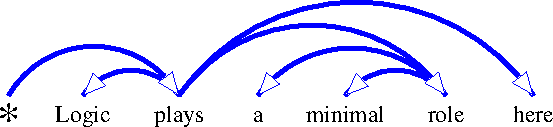
\includegraphics[width=0.6\columnwidth]{img/example_proj_logic01}
}
\end{center}
\begin{itemize}
\item<1-> A lexicalized syntactic formalism
\item<1-> Grammar functions represented as lexical relationships (dependencies)
\end{itemize}
\item[] {\scriptsize{\citep{Eisner1996,McDonald2005b,Nivre2006CoNLL,Koo2007}}}
\end{itemize}
\end{frame}
\end{comment}


\begin{frame}%
\frametitle{Examples of structure in NLP}%
\small%
\makebox[\textwidth][c] {%  center three miniboxes on slide
\onslide<3>%
\begin{minipage}[t][][c]{.31\textwidth}
\centering
{\Large POS tagging}\\
\bigskip
\postag{VERB}{PREP}{NOUN}\\[5.5ex]
\postag{NOUN}{PREP}{NOUN}\\[5.5ex]
\postag{NOUN}{DET}{NOUN}\\
\end{minipage}
\onslide<1->
\begin{minipage}[t][][c]{.40\textwidth}  % 36 min
\centering
{\Large Dependency parsing}\\
\bigskip
$\cdots$\\[1ex]
\simpledep{$\star$ \& dog \& on \& wheels \\}{
\depedge{1}{2}{}
\depedge{2}{3}{}
\depedge{3}{4}{}
}
\\[1ex]
\simpledep{$\star$ \& dog \& on \& wheels \\}{
\depedge{1}{4}{}
\depedge{4}{2}{}
\depedge{4}{3}{}
}
\\[2ex]
\simpledep{$\star$ \& dog \& on \& wheels \\}{
\depedge{1}{2}{}
\depedge{2}{3}{}
\depedge{2}{4}{}
}\\$\cdots$
\end{minipage}
\onslide<3>
\begin{minipage}[t][][c]{.28\textwidth}
\centering
{\Large Word alignments}\\
\bigskip
\matching{2,1,3}
\\[2ex]
\matching{1,2,3}
\\[2ex]
\matching{3,1,2}\\
\end{minipage}}

\onslide<2>\overlaybox{%
\\
\\
{\LARGE Exponentially many parse trees!}\\
\\
{\LARGE Cannot enumerate.}
\\
}

\end{frame}


\begin{frame}[plain]
\frametitle{NLP 5 years ago:}
\framesubtitle{Structured prediction and pipelines}

\begin{center}
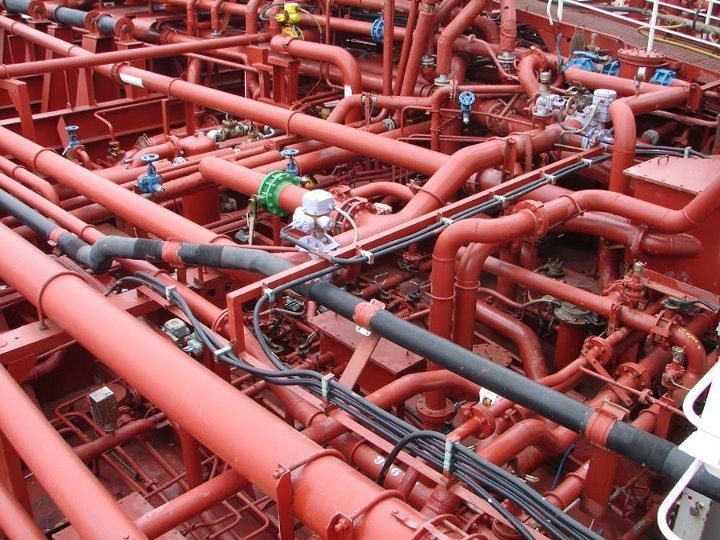
\includegraphics[width=1.\columnwidth]{img/pipeline.jpg}
\end{center}

\end{frame}

\begin{frame}
\frametitle{NLP 5 years ago:}
\framesubtitle{Structured prediction and pipelines}

\begin{itemize}
\item Big pipeline systems, connecting different structured predictors, trained separately
\item {\bf Advantages:} fast and simple to train, can rearrange pieces \emoji{happ}
\item<2-> {\bf Disadvantage:} linguistic annotations required for each component \emoji{sweat}
\item<3-> {\bf Bigger disadvantage:} error propagates through the pipeline \emoji{poop}
\end{itemize}

\end{frame}


\begin{frame}[plain]
\frametitle{NLP today:}
\framesubtitle{End-to-end training}
\begin{center}
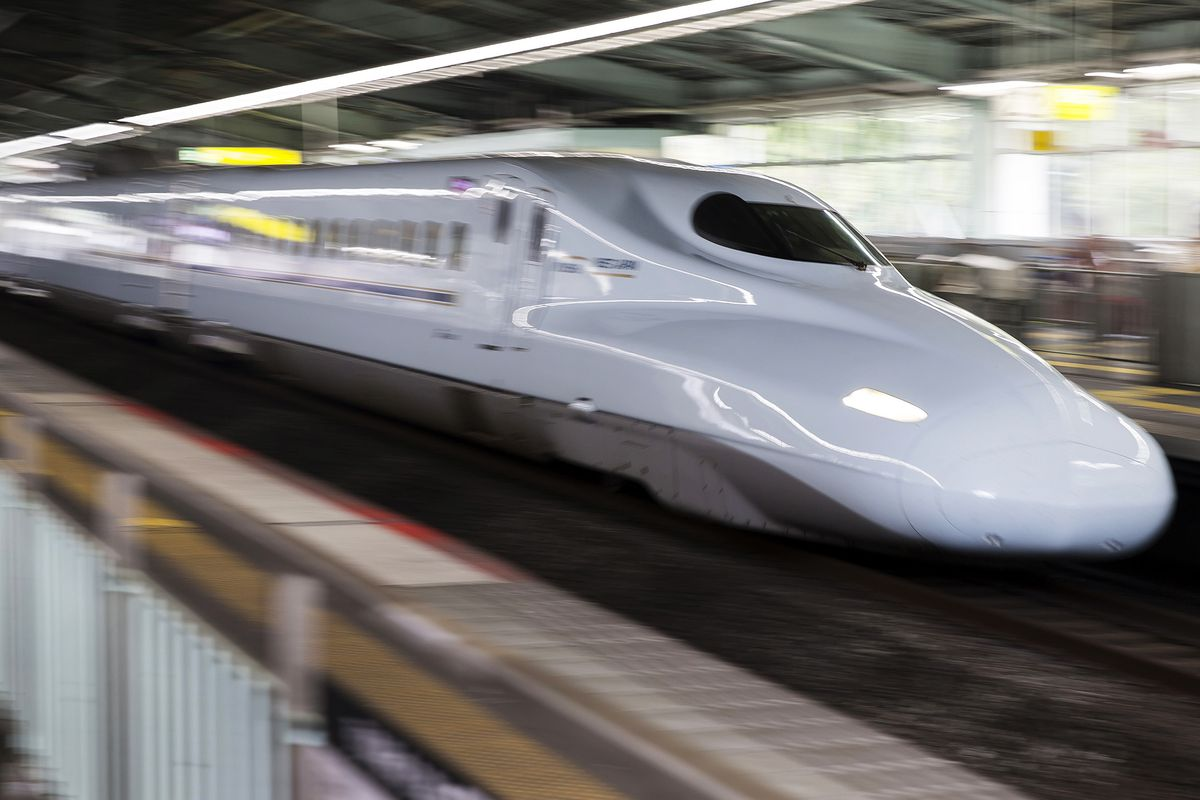
\includegraphics[width=1.\columnwidth]{img/end_to_end_train.jpg}
\end{center}
\end{frame}


\begin{frame}
\frametitle{NLP today:}
\framesubtitle{End-to-end training}

\begin{itemize}
\item Forget pipelines---train everything from scratch!
\item No more error propagation or linguistic annotations! \emoji{party}
\item<2-> Treat everything as \emph{latent}! \emoji{palms}
%\item ... with a little bit of inductive bias to promote the kind of structures we want
\end{itemize}
\end{frame}

%\begin{frame}
%\frametitle{Latent Structure Models}
%
%\begin{itemize}
%\item To be fair, latent structure models were not invented only in the last 5 years.
%\item Example: IBM Models for SMT (latent word alignments).
%\item The ``classical'' approach was based on:
%\begin{itemize}
%\item Generative models trained with the EM algorithm \citep{petrov2008discriminative,ganchev2010posterior}
%\item CRFs with hidden variables \citep{quattoni2007hidden}
%\item Spectral learning and method of moments \citep{hsu2012spectral,anandkumar2012spectral,cohen2012spectral}
%\item Some semi-supervision sometimes \citep{marinho2016semi}
%\end{itemize}
%\item Often, these models make very strict assumptions (e.g. strong factorizations)
%\item Today, neural networks opened up some new possibilities!
%\end{itemize}
%
%\end{frame}


\begin{frame}%
\frametitle{Representation learning}%
\makebox[\textwidth][c] {% two boxes
\begin{minipage}[t][][c]{.45\textwidth}
\begin{itemize}%
\item Uncover hidden representations useful for the \emph{downstream task}.
\item<1-> Neural networks are well-suited for this: \emph{deep computation graphs}.
\item<2-> Neural representations are unstructured, inscrutable. Language data
has underlying structure!
\end{itemize}%
\end{minipage}%
\hfill%
%
\begin{minipage}[t][][c]{.5\textwidth}
\centering
\begin{tikzpicture}[node distance=5pt,inner sep=1pt,scale=.3]
\draw[myfg,thick,fill=mygr!25!mybg] (4.5, 0) rectangle (8.5, 9) {};
\draw[rounded corners,myfg,very thick] (0, 0) rectangle (13, 9) {};
\node[align=center] (In) at (-2, 4.5) {\Huge \faicon{envelope-o}};
\node[align=center] (Out) at (17, 4.5) {\usebox{\sentoutputsmall}};
\node[align=center,above=of In] {\small input};
\node[align=center] at (6.5, 4.5) {}; %{\only<1>{\Huge \faicon{map-o}}};
\path (2.25, 4.5) pic[scale=.25] {cog};
\path (10.75, 4.5) pic[scale=.25] {cog};
%\node[anchor=south west] at (4.5, 0) {$h$};
\only<1->{
\pgfmathsetseed{42}
\foreach \i in {0,1,2,...,8}{
  \pgfmathparse{75*rand}
  \fill[tDY!\pgfmathresult!tPink]  (6, \i) rectangle (7, \i+1) {};
}
\draw[black,thick] (6, 0) rectangle (7, 9) {};
}
\end{tikzpicture}%
\end{minipage}}
\end{frame}
%

\begin{frame}
\frametitle{\only<1->{Latent structure models}}
\makebox[\textwidth][c] {% two boxes
\begin{minipage}[t][][c]{.45\textwidth}
\begin{itemize}%
\item<1-> Seek \emph{structured} hidden representations instead!
\end{itemize}%
\end{minipage}%
\hfill%
%
\begin{minipage}[t][][c]{.5\textwidth}
\centering
\begin{tikzpicture}[node distance=5pt,inner sep=1pt,scale=.3]
\draw[myfg,thick,fill=mygr!25!mybg] (4.5, 0) rectangle (8.5, 9) {};
\draw[rounded corners,myfg,very thick] (0, 0) rectangle (13, 9) {};
\node[align=center] (In) at (-2, 4.5) {\Huge \faicon{envelope-o}};
\node[align=center] (Out) at (17, 4.5) {\usebox{\sentoutputsmall}};
\node[align=center,above=of In] {\small input};
\only<2->{%
\node[align=center,font=\small] at (6.5, 4.5) {%
    $\cdots$\\[-1pt]
    \cartoon[.4]{1/4}\\[1pt]%
    \cartoon[.7]{1/2,1/4}\\[1pt]%
    \cartoon[.4]{2/3,3/4}\\[-3pt]%
    $\cdots$};
}
\path (2.25, 4.5) pic[scale=.25] {cog};
\path (10.75, 4.5) pic[scale=.25] {cog};
%\node[anchor=south west] at (4.5, 0) {$h$};
\only<1>{
\pgfmathsetseed{42}
\foreach \i in {0,1,2,...,8}{
  \pgfmathparse{75*rand}
  \fill[tDY!\pgfmathresult!tPink]  (6, \i) rectangle (7, \i+1) {};
}
\draw[black,thick] (6, 0) rectangle (7, 9) {};
}
\end{tikzpicture}%
\end{minipage}}
\end{frame}

\begin{frame}
\frametitle{Latent structure models aren't so new!}

\begin{itemize}
\item They have a very long history in NLP:
\begin{itemize}
\item IBM Models for SMT (latent word alignments) \citep{brown1993mathematics}
\item HMMs \citep{Rabiner1989}
\item CRFs with hidden variables \citep{quattoni2007hidden}
\item Latent PCFGs \citep{petrov2008discriminative,cohen2012spectral}
\end{itemize}
\item Trained with EM, spectral learning, method of moments, ... \\
%\citep{hsu2012spectral,anandkumar2012spectral,cohen2012spectral,marinho2016semi}
\item Often, very strict assumptions (e.g. strong factorizations)
\item Today, neural networks opened up some new possibilities!
\end{itemize}

\end{frame}


\begin{frame}%
\frametitle{Why do we love latent structure models?}%

\begin{itemize}
\item The inferred latent variables can bring us some {\bf interpretability}
\item They offer a way of injecting prior knowledge as a {\bf structured bias}
\item Hopefully: Higher predictive power with fewer model parameters
\begin{itemize}
\item<2->{\alert{smaller carbon footprint!}}
\end{itemize}
\end{itemize}

\end{frame}


\begin{frame}
\frametitle{What this tutorial is about:}

\begin{itemize}
\item Discrete, combinatorial latent structures
\item Often the structure is inspired by some linguistic intuition
%\item But no supervision beyond this structured induction bias!
\item We'll cover both:
\begin{itemize}
\item RL methods (structure built incrementally, reward coming from downstream task)
\item ... vs end-to-end differentiable approaches (global optimization, marginalization)
\item stochastic computation graphs
\item ... vs deterministic graphs.
\end{itemize}
\item All plugged in \emph{discriminative} neural models.
\end{itemize}
\end{frame}


\begin{frame}
\frametitle{This tutorial is \emph{not} about:}

\begin{itemize}
\item It's not about continuous latent variables
\item It's not about deep generative learning
\item We won't cover GANs, VAEs, etc.
\item There are (very good) recent tutorials on deep variational models for NLP:
\begin{itemize}
\item ``Variational Inference and Deep Generative Models'' (Schulz and Aziz, ACL 2018)
%http://wilkeraziz.github.io/vitutorial.html
\item ``Deep Latent-Variable Models for Natural Language'' (Kim, Wiseman, Rush, EMNLP 2018)
%http://nlp.seas.harvard.edu/latent-nlp-tutorial.html
\end{itemize}
\end{itemize}

\end{frame}


\sepframe[mygr]{Background}

\begin{frame}%
\frametitle{Unstructured vs structured}%

\begin{itemize}
\item To better explain the math, we'll often backtrack to \emph{unstructured} models (where the latent variable is a categorical) before jumping to the \emph{structured} ones
\end{itemize}
\end{frame}


\begin{frame}
\frametitle{The unstructured case: Probability simplex}

\begin{columns}[t]%
\begin{column}{.3\textwidth}%
\begin{tikzpicture}[baseline=(current bounding box.north)]
\setupsimplexbary{}
\coordinate (argmax)    at (barycentric cs:L1=0,L2=0,L3=1);
\coordinate (softmax)   at (barycentric cs:L1=.3,L2=.2,L3=.5);
%\coordinate (sparsemax) at (barycentric cs:L1=.3,L2=0,L3=.7);

\uncover<2->{%
\node[label=west:{\small $[0,0,1]$}] at (argmax) {};
\draw[point,fill=colorArgmax] (argmax) circle[radius=5pt];}
\uncover<3->{%
\node[label=south:{\small $[.3,.2,.5]$}] at (softmax) {};
\draw[point,fill=colorSoftmax] (softmax) circle[radius=5pt];}
\end{tikzpicture}%

\end{column}
\begin{column}{.5\textwidth}%
\begin{itemize}
\item<2-> Each vertex is an \emph{indicator vector}, representing one class:
\begin{equation*}
\z_c = [0, \ldots, 0, \underbrace{1}_{c\text{\textsuperscript{th} position}}, 0, \ldots, 0].
\end{equation*}
\item<3-> Points inside are \emph{probability vectors}, a convex combination of classes:
\begin{equation*}
\p \ge \mathbf{0}, \,\, \sum_c \pp_c = 1.
\end{equation*}
\end{itemize}
\end{column}
\end{columns}

\end{frame}%


\begin{frame}%
\frametitle{What's the analogous of $\triangle$ for a structure?}%

\begin{itemize}
\item A structured object $\bs{z}$ can be represented as a \emph{bit vector}.
\item<2-> Example:
\begin{itemize}
\item<2-> a dependency tree can be represented a $O(L^2)$ vector indexed by arcs
\item<2-> each entry is 1 iff the arc belongs to the tree
\item<2-> {\bf structural constraints:} not all bit vectors represent valid trees!
\end{itemize}
\end{itemize}

\bigskip

\uncover<3->{
\begin{center}
\begin{columns}
\begin{column}{0.3\columnwidth}
\small
$\z_1 = [\textcolor{tPink}{1}, 0, 0, 0, \textcolor{tPink}{1}, 0, 0, 0, \textcolor{tPink}{1}]$\\

\simpledep{$\star$ \& dog \& on \& wheels \\}{
\depedge{1}{2}{}
\depedge{2}{3}{}
\depedge{3}{4}{}
}
\end{column}
\begin{column}{0.3\columnwidth}
\small
$\z_2 = [0, 0, \textcolor{tPink}{1}, 0, 0, \textcolor{tPink}{1}, \textcolor{tPink}{1}, 0, 0]$\\

\simpledep{$\star$ \& dog \& on \& wheels \\}{
\depedge{1}{4}{}
\depedge{4}{2}{}
\depedge{4}{3}{}
}
\end{column}
\begin{column}{0.3\columnwidth}
\small
$\z_3 = [\textcolor{tPink}{1}, 0, 0, 0, \textcolor{tPink}{1}, 0, 0, \textcolor{tPink}{1}, 0]$\\

\simpledep{$\star$ \& dog \& on \& wheels \\}{
\depedge{1}{2}{}
\depedge{2}{3}{}
\depedge{2}{4}{}
}
\end{column}
\end{columns}

\end{center}
}

\end{frame}%

\begin{frame}[label=marginalpoly]%
\frametitle{The structured case: Marginal polytope}%
\cornercite{Wainwright2008}%
\centering

%\begin{itemize}
%\item A structured object $\bs{y}$ (e.g. a dependency tree) can be represented as a \emph{bit vector}.
%\begin{itemize}
%\item e.g. a $O(L^2)$ vector indexed by arcs, where each entry is 1 iff the arc belongs to the tree.
%\end{itemize}
%\end{itemize}

\begin{columns}[t]%
\begin{column}{.7\textwidth}%
\begin{itemize}
    \item<2-> Each vertex corresponds to one such \emph{bit vector} $\z$
    \item<3-> Points inside correspond to \emph{marginal distributions}: convex combinations of structured objects
\begin{equation*}
\mg = \underbrace{{\pp_1} \z_1 + \ldots + {\pp_N} \z_N}_{\text{exponentially many terms}}, \,\, \p \in \Delta.
\end{equation*}

{\small
\begin{equation*}
\begin{array}{ll}
\pp_1 = 0.2, & \z_1 = [\textcolor{tPink}{1}, 0, 0, 0, \textcolor{tPink}{1}, 0, 0, 0, \textcolor{tPink}{1}]\\
\pp_2 = 0.7, & \z_2 = [0, 0, \textcolor{tPink}{1}, 0, 0, \textcolor{tPink}{1}, \textcolor{tPink}{1}, 0, 0]\\
\pp_3 = 0.1, & \z_3 = [\textcolor{tPink}{1}, 0, 0, 0, \textcolor{tPink}{1}, 0, 0, \textcolor{tPink}{1}, 0]\\
\end{array}
\quad \Rightarrow \quad
\mg = [\textcolor{tPink}{.3}, 0, \textcolor{tPink}{.7}, 0, \textcolor{tPink}{.3}, \textcolor{tPink}{.7}, \textcolor{tPink}{.7}, \textcolor{tPink}{.1}, \textcolor{tPink}{.2}].
\end{equation*}
}

%\begin{itemize}
%\item<3-> e.g. each entry $\mu_a$ %= \sum_{\text{tree} \ni a} p(\text{tree})$
%is the marginal probability of arc $a$, given a distribution $\bs{p}$ over trees.
%\end{itemize}
\end{itemize}

\end{column}
\begin{column}[T]{.3\textwidth}%
\centering
\begin{tikzpicture}
\node[
    ultra thick,
    draw=colorPolytope,
    fill=colorPolytope,
    fill opacity=.15,
    minimum size=2.5cm,
    regular polygon, regular polygon sides=6] (mp) {};
\node[label=east:{\small$\mathcal{M}$}] at (mp.corner 5) {};
\foreach \i in {1, ..., 6}%
{
    \draw[colorPolytope,fill] (mp.corner \i) circle[radius=3pt];
}

\onslide<2->{
    \draw[point,fill=colorArgmax] (.6,1.1) circle[radius=5pt];
    \node at (1.5,1) {\cartoon[.5]{1/4,2/5}};
}

\onslide<3->{
    \draw[point,fill=colorSoftmax] (-.2,-.1) circle[radius=5pt];
    \node at (-2, -.5) {\cartoonDense[.5]{}};
}
\end{tikzpicture}
\end{column}
\end{columns}
\end{frame}


\begin{frame}{Unstructured vs Structured}

\begin{columns}[T]%
\begin{column}{.45\textwidth}\centering%
\vbox to .7\textheight{%

\begin{itemize}
\item Unstructured case: simplex $\Delta$
\end{itemize}

\vfill

\begin{tikzpicture}
\setupsimplexbary[2.5]{}
\coordinate (argmax)    at (barycentric cs:L1=0,L2=0,L3=1);
\coordinate (softmax)   at (barycentric cs:L1=.3,L2=.2,L3=.5);
\coordinate (sparsemax) at (barycentric cs:L1=.3,L2=0,L3=.7);

\onslide<2->{
\draw[point,fill=colorArgmax] (argmax) circle[radius=5pt];
}
\onslide<3->{
\draw[point,fill=colorSoftmax] (softmax) circle[radius=5pt];
}
%\onslide<8->{
%\draw[point,fill=colorSparsemax] (sparsemax) circle[radius=5pt];
%}
\end{tikzpicture}}
\end{column}
\begin{column}{.54\textwidth}\centering
\vbox to .7\textheight{%

\begin{itemize}
\item Structured case: marginal polytope $\mathcal{M}$
\end{itemize}

\vfill
\begin{tikzpicture}[node distance=0pt]%
\uncover<1->{
\node[
    ultra thick,
    draw=colorPolytope,
    fill=colorPolytope,
    fill opacity=.15,
    minimum size=2.5cm,
    regular polygon, regular polygon sides=6] (mp) {};
\node[label=east:{\small$\mathcal{M}$}] at (mp.corner 5) {};
\foreach \i in {1, ..., 6}%
{
    \draw[colorPolytope,fill] (mp.corner \i) circle[radius=3pt];
}
}
\coordinate (L1) at (mp.corner 3);
\coordinate (L2) at (mp.corner 5);
\coordinate (L3) at (mp.corner 2);
\coordinate (argmax)    at (L3);
\coordinate (softmax)   at (barycentric cs:L1=.25,L2=.25,L3=.45);
%\coordinate (sparsemax) at (barycentric cs:L1=.4,L3=.6);
\onslide<2->{
    \draw[point,fill=colorArgmax] (argmax) circle[radius=5pt];
    \node[above right=of argmax] {\cartoon[.5]{1/4,2/5}};
}
\onslide<3->{
    \draw[point,fill=colorSoftmax] (softmax) circle[radius=5pt];
    \node[below right=of softmax] {\cartoonDense[.5]{}};
}
%\onslide<9->{
%    \draw[point,fill=colorSparsemax] (sparsemax) circle[radius=5pt];
%    \node[left=of sparsemax] {\cartoonSparse[.5]{}};
%}
\end{tikzpicture}}
\end{column}
\end{columns}

\end{frame}


\begin{frame}
\frametitle{Computing the most likely structure}
\framesubtitle{is a very high-dimensional argmax}
\centering
\begin{tikzpicture}
    \node[anchor=south] at (0, \vecheight*4) {\cartoon[.66]{1/4}};
    \node[anchor=south] at (0, \vecheight*2.5) {\cartoon[.66]{1/2,1/4}};
    \node[anchor=south] at (0, \vecheight*1.5) {$\cdots$};
    \node[anchor=south] at (0, \vecheight*0) {\cartoon[.66]{2/3,2/4}};
\drawscores
\drawargmax[\z]

\node[anchor=south,align=center] at (-6, \vecheight*3+1) (in) {input\\$\bs{x}$};
\node[anchor=south] at (-2, \vecheight*3+1) (in-end) {};
\node[anchor=south,align=center] at (6, \vecheight*3+1)
(out){output\\$\widehat{\bs{y}}$};
\node[anchor=south] at (2, \vecheight*3+1) (out-end) {};
\path (in) edge[->,very thick,bend right=50] (in-end);
\node[anchor=south] at (4, \vecheight*3+.9) (out-mid) {
    \cartoon[.9]{1/2,1/4}
};
\path (out-end) edge[->,very thick,bend right=50] (out-mid.south west);
\path (out-mid.south east) edge[->,very thick,bend right=50] (out);
\end{tikzpicture}

\onslide<2->\overlaybox{%
    There are exponentially\\many structures\\
    {\small ($\s$ cannot fit in memory;}\\
    {\small we cannot ``loop'' over $\s$ nor $\z$)}
}
\end{frame}

\begin{frame}[t,label=structuretypes]%
\frametitle{Dealing with the combinatorial explosion}
\begin{columns}[t]%
\begin{column}{.5\textwidth}%
\centering%
\cartoon[.7]{1/2} $\rightarrow$
\cartoon[.7]{1/2,1/5} $\rightarrow$
\cartoon[.7]{1/2,1/5,1/3} $\rightarrow \cdots$
\\[\baselineskip]
\textbf{1. Incremental structures} \\
\begin{itemize}
\item Build structure \textbf{greedily}, as sequence of discrete choices
(e.g., shift-reduce).
\item Scores (partial structure, action) tuples.
\item {\bf Advantages:} flexible, rich histories.
\item {\bf Disadvantages:} greedy, local decisions are suboptimal,
error propagation.
\end{itemize}
\end{column}
\begin{column}{.5\textwidth}%
\centering%
$\max\big\{\cdots$,
\cartoon[.7]{1/2,1/5,1/3,1/4},
\cartoon[.7]{1/2,1/5,1/3,3/4},
\cartoon[.7]{1/2,1/5,1/3,5/4},
$\cdots\big\}$
\\[\baselineskip]

\textbf{2. Factorization into parts} \\
\begin{itemize}
%\item[] $$ \mg = \bs{A} \p $$
\item Optimizes \textbf{globally} (e.g.\ Viterbi, Chu-Liu-Edmonds,
Kuhn-Munkres).
\item Scores smaller parts.\\
\item {\bf Advantages:} optimal, elegant, can handle hard \& global constraints.
\item {\bf Disadvantages:} strong assumptions.
\end{itemize}
\end{column}
\end{columns}
\end{frame}


\begin{frame}%
\frametitle{The challenge of discrete choices.}%
\centering%
\begin{tikzpicture}
\drawcs
\onslide<2->{\drawscores}
\onslide<3->{\drawargmax[\z]}
%
\onslide<4->{
    \node[anchor=south,align=center] at (-6, \vecheight*3+1) (in) {input\\$\bs{x}$};
\node[anchor=south] at (-2, \vecheight*3+1) (in-end) {};
\node[anchor=south,align=center] at (6, \vecheight*3+1) (out){output\\$\widehat{\bs{y}}$};
\node[anchor=south] at (2, \vecheight*3+1) (out-end) {};
%
\path (in) edge[->,very thick,bend right=50] node[anchor=north] {$\s =
    \bs{f}_{\parp}(\bs{x})$} (in-end);
\path (out-end) edge[->,very thick,bend right=50] node[anchor=north] {$\widehat{\bs{y}} =
    \bs{g}_{\clfp}(\z, \bs{x})$} (out);
}
%
\node at (0, -1) {{%
\onslide<5->{$\frac{\partial L(\widehat{\bs{y}},\bs{y})}{\partial \bs{w}} = ?$}
\onslide<6->{\quad or, essentially, \quad $\frac{\partial \z}{\partial \s}=?$}
}};\end{tikzpicture}
\end{frame}


\begin{frame}%
\frametitle{Discrete mappings are ``flat''}%
\centering%
\begin{tikzpicture}%
%
\node[anchor=south] at (-1-.5*\vecwidth, \vecheight*5+.1) {$\s$};

\drawcs
\drawscores
\drawargmax[\z]

\foreach[count=\i] \x in {64,69,74,79,84,89,94,99}{
    \onslide<\i>{
        \draw[elem,fill=vecfg!\x!vecbg] (-1-\vecwidth, \vecheight*4) rectangle (-1, \vecheight*5);}
}

\node[anchor=south] at (1+.5*\vecwidth, \vecheight*5+.1) {$\z$};
\foreach[count=\i] \x in {64,69,74,79,84,89,94,99}{
\onslide<\i>{
\draw[elem,fill=vecfg!%
\ifnum\x<85
    0
\else
    70
\fi!vecbg]  (1, \vecheight*4) rectangle (1+\vecwidth, \vecheight*5);
%
\draw[elem,fill=vecfg!%
\ifnum\x<85
    70
\else
    0
\fi!vecbg] (1, \vecheight*3) rectangle (1+\vecwidth, \vecheight*4);
}}

\node[anchor=south,align=center] at (-6, \vecheight*3+1) (in) {\phantom{input}};
\node[anchor=south,align=center] at (6, \vecheight*3+1) (out) {\phantom{output}};
%
\node at (0, -1) {$\frac{\partial \z}{\partial \s}=?$};
\end{tikzpicture}\end{frame}

\begin{frame}%
\frametitle{Argmax}
\centering%
\begin{tikzpicture}%
%
\drawcs\drawscores\drawargmax[\z]
%
\node at (0, -1) {$\frac{\partial \z}{\partial \s}=\bs{0}$};
\node[anchor=south,align=center] at (-6, \vecheight*2+1) (in) {\phantom{input}};
\node[anchor=south,align=center] at (6, \vecheight*2+1) (out) {\phantom{output}};
\end{tikzpicture}%
\\[-\baselineskip]

\begin{tikzpicture}[overlay]
    \draw[axisline,->] (3, 3) -- (3, 6) node[left] {$\zz_1$};
    \draw[axisline,->] (3, 3) -- (7, 3) node[right]{$\ss_1$};

    \node[axislabel,left] at (3, 3) {$0$};
    \node[axislabel,left] at (3, 5) {$1$};

    \draw[axisline] ($(3,3) + (-\ticksize, 0)$) -- ($(3,3) + (+\ticksize, 0)$);
    \draw[axisline] ($(3,4) + (-\ticksize, 0)$) -- ($(3,4) + (+\ticksize, 0)$);
    \draw[axisline] ($(3,5) + (-\ticksize, 0)$) -- ($(3,5) + (+\ticksize, 0)$);

    \draw[axisline] ($(3,3) + (0, -\ticksize)$) -- ($(3,3) + (0, +\ticksize)$);
    \draw[axisline] ($(4,3) + (0, -\ticksize)$) -- ($(4,3) + (0, +\ticksize)$);
    \draw[axisline] ($(5,3) + (0, -\ticksize)$) -- ($(5,3) + (0, +\ticksize)$);
    \draw[axisline] ($(6,3) + (0, -\ticksize)$) -- ($(6,3) + (0, +\ticksize)$);

    \node[axislabel,below] at (4, 3) {$\ss_2 - 1$};
    \node[axislabel,below] at (5, 3) {$\ss_2$};
    \node[axislabel,below] at (6, 3) {$\ss_2 + 1$};

    \draw[ultra thick,colorArgmax] (3, 3) -- (5,3) ;
    \draw[ultra thick,colorArgmax] (5, 5) -- (7,5) ;
\end{tikzpicture}
\end{frame}


% \begin{frame}%
% \frametitle{Continuous Relaxation via Softmax}
% \centering%
% \begin{tikzpicture}%
% %
% \drawcs\drawscores\drawsoftmax
% \node at (0, -1) {$\frac{\partial \p}{\partial \s}=\operatorname{diag}(\p) - \p\p^\top$};
% \node[anchor=south,align=center] at (-6, \vecheight*2+1) (in) {\phantom{input}};
% \node[anchor=south,align=center] at (6, \vecheight*2+1) (out) {\phantom{output}};
% \end{tikzpicture}
% \\[-\baselineskip]
%
% \begin{tikzpicture}[overlay]
%     \draw[axisline,->] (3, 3) -- (3, 6) node[left] {$p_1$};
%     \draw[axisline,->] (3, 3) -- (7, 3) node[right]{$\theta_1$};
%
%     \node[axislabel,left] at (3, 3) {$0$};
%     \node[axislabel,left] at (3, 5) {$1$};
%
%     \draw[axisline] ($(3,3) + (-\ticksize, 0)$) -- ($(3,3) + (+\ticksize, 0)$);
%     \draw[axisline] ($(3,4) + (-\ticksize, 0)$) -- ($(3,4) + (+\ticksize, 0)$);
%     \draw[axisline] ($(3,5) + (-\ticksize, 0)$) -- ($(3,5) + (+\ticksize, 0)$);
%
%     \draw[axisline] ($(3,3) + (0, -\ticksize)$) -- ($(3,3) + (0, +\ticksize)$);
%     \draw[axisline] ($(4,3) + (0, -\ticksize)$) -- ($(4,3) + (0, +\ticksize)$);
%     \draw[axisline] ($(5,3) + (0, -\ticksize)$) -- ($(5,3) + (0, +\ticksize)$);
%     \draw[axisline] ($(6,3) + (0, -\ticksize)$) -- ($(6,3) + (0, +\ticksize)$);
%
%     \node[axislabel,below] at (4, 3) {$\theta_2 - 1$};
%     \node[axislabel,below] at (5, 3) {$\theta_2$};
%     \node[axislabel,below] at (6, 3) {$\theta_2 + 1$};
%
%     \draw[ultra thick,colorArgmax] (3, 3) -- (5,3) ;
%     \draw[ultra thick,colorArgmax] (5, 5) -- (7,5) ;
%
%     \draw (3, 3.1) edge[colorSoftmax,ultra thick,out=360,in=180,looseness=1.5] (7, 4.9);
%
%     \node[anchor=south,align=center] at (-5, 4) (in) {$p_j = \exp(\theta_j) / Z$};
%     %\node[anchor=south,align=center] at (-5, 4) (in) {$p_j \coloneqq \exp(\theta_j) / Z$};
%
% \end{tikzpicture}%
% \end{frame}


\begin{frame}%
\colorlet{patcol}{black!60!white}
\tikzset{
    nosep/.style = {inner sep=0, outer sep=0},
    vec/.style = {draw,rectangle,minimum width=5pt,minimum height=30pt},
    wva/.style = {fill=mygr},
    wvb/.style = {fill=mygr},
    grad/.style = {color=tGreen,very thick},
    nograd/.style = {color=tPink,very thick},
    fwd/.style = {very thick, color=mygr}
}
\frametitle{Example: Regression with latent categorization}%
\centering%
{
\pgfdeclarelayer{bg}    % declare background layer
\pgfsetlayers{bg,main}  % set the order of the layers (main is the standard layer)
\begin{tikzpicture}

\uncover<1->{\drawscores}
\uncover<2-11>{\drawargmax[\z]}
\uncover<12>{\drawsoftmax}
%
\node[anchor=north,align=center] at (-6, \vecheight*1+3) (in)
{{\small input $\bs{x}$} \\ \faicon{envelope-o}};

%%% Left half
%%%%%%%%%%%%%

% h vector
\node[vec,wva,right=of in,outer sep=5pt,label={\small $\bs{u}$}] (h) {};

% embedding matrix
\node[below=60pt of in,align=center,anchor=south] (embed)
    {\faListAlt\\[-.25\baselineskip]{\small embeddings $\bs{E}$}};
% w_theta
\node[right=of embed.south east,anchor=south west] (wth) {\small $\bs{W}_{\s}$};

% arrows among left half
\node[right=45pt of h] (in-end) {};
\begin{pgfonlayer}{bg}
\path (in) edge[fwd,->] node[nosep] (inhmid) {} (h);
\path (h) edge[fwd,->] node[nosep] (inthetamid) {} (in-end);
\path (embed) edge[fwd,bend left=25] (inhmid);
\path (wth) edge[fwd,bend left=30] (inthetamid);
\end{pgfonlayer}

% Bottom left
\node [nosep,below=10pt of embed.south,anchor=north,minimum height=20pt] {\small $\bs{u} = \frac{1}{|\bs{x}|} \sum_j \bs{E}_{x_j}$};
\node [nosep,below=10pt of wth.south,anchor=north,minimum height=20pt]
(thetadef) {\small $\s =  \bs{W}_{\s} \bs{u}$};

%%% Right half
%%%%%%%%%%%%%%

\uncover<3->{%
\node[anchor=north,minimum height=20pt,text depth=20pt,align=center] at (+6, \vecheight*1+3) (out)
{\small output $\hat{y}$};
\node[vec,wvb,left=of out,outer sep=5pt,label={\small $\bs{v}$}] (g) {};
\node[left=40pt of g] (out-end) {};

% arrows among right
\path (out-end) edge[fwd,->] node[nosep] (pgmid) {} (g);
\path (g) edge[fwd,->] node[nosep] (gymid) {} (out);

\node[below=60pt of pgmid,anchor=north] (wg) {\small $\bs{W}_{\bs{v}}$};
\node[below=60pt of gymid,anchor=north] (wy) {\small $\bs{W}_y$};

\node [nosep,right=60pt of thetadef,minimum height=20pt] (glbl)
    {\small $\bs{v} = \operatorname{tanh}\left(%
\bs{W}_{\bs{v}}[\bs{u}, \alt<12>{\p}{\z}]
%\alt<12>{\p}{\z}^\top \bs{W}_{\bs{g}})
%{\bs{h}}
\right)$};
\node [nosep,right=90pt of glbl.west,minimum height=20pt] (ylbl) {\small $\hat{y} = \bs{W}_y \bs{v}$};
\node [nosep,right=40pt of ylbl.west,minimum height=20pt] (loss) {\small $L =
%
\only<10>{\textcolor{tGreen}{\EE_{\z}}}
%
(\hat{y} - y)^2$};
}
\uncover<8>{
    \node[tGreen,above=-8pt of loss.north east] (semisuploss)
        {\small $-\log \frac{\exp({\ss}_c)}{Z}$};
%        \path (semisuploss) edge[grad,->,bend left=5] (wth);
%        \path (semisuploss) edge[grad,->,bend left=5] (embed);
}

\begin{pgfonlayer}{bg}
\uncover<2->{\node[anchor=south] at (.5, \vecheight*3) {\small $(c)$};}

% this line go away when we reparametrize
\uncover<3->{%
\path (h) edge[fwd, bend left=20] (pgmid);
\path (wg) edge[fwd,bend left=30] (pgmid);
\path (wy) edge[fwd,bend left=30] (gymid);
}

\uncover<4->{%
\node[below=5pt of out.west,nosep] (gradorigin) {};
\node[below=5pt of pgmid,nosep] (gradpgmid) {};
\node[below=5pt of inthetamid,nosep] (gradinthetamid) {};
\node[above=0pt of pgmid] (gradpgmidtop) {};
\node[above=5pt of h.east] (gradh) {};
\node[below=10pt of inhmid] (gradinhmid) {};
\path (gradorigin) edge[grad,->,bend right=20] (wy);
\path (gradorigin) edge[grad] (gradpgmid);
\path (gradpgmid) edge[grad,->,bend right=20] (wg);
\path (h) edge[grad,->,bend right=15] (embed);
}
% this line goes away when we reparametrize
\uncover<4-8>{%
\path (gradpgmidtop) edge[grad,->, bend right=20] (gradh);
}
\uncover<5-9>{
\path (gradpgmid) edge[nograd] (gradinthetamid);
\path (gradinthetamid) edge[nograd,->,bend right=20] (wth);
}
\uncover<8>{
\path (.5, \vecheight*3) edge[grad,dashed,->,bend right=20] (wth);
}
%\uncover<9-10>{
%\node[right=10pt of in-end] (threp) {};
%\path (threp) edge[fwd,dashed,bend left=20] (g.west);
%\path ([yshift=5pt]g.west) edge[grad,dashed,->,bend right=20] ([yshift=5pt]threp);
%\path (in-end) edge[grad,dashed,->,bend right=20] (wth);
%}
\uncover<10->{
\path (gradpgmid) edge[grad] (gradinthetamid);
\path (gradinthetamid) edge[grad,->,bend right=20] (wth);
}
\end{pgfonlayer}
\uncover<5>{
    \node[draw,minimum width=20pt,tPink,rectangle] (wthborder) at (wth) {};
}
\end{tikzpicture}
}%
\\[.5\baselineskip]
\begin{overlayarea}{\linewidth}{3\baselineskip}
\centering%
\only<2-3>{predict topic $c$ ($\bs{z} = \bs{e}_c$)}
\only<5>{%
\small
$\pfrac{L}{\bs{W}_{\s}}=
\pfrac{L}{\hat{y}}~
\pfrac{\hat{y}}{\bs{v}}~
\pfrac{\bs{v}}{\bs{z}}
\overbrace{\textstyle\textcolor{tPink}{\pfrac{\z}{\s}}}^{\equiv 0}
\pfrac{\s}{\bs{W}_{\s}}
$}
\only<7>{Option 1. Pretrain latent classifier $\bs{W}_{\s}$}
\only<8>{Option 2. Multi-task learning}
%\only<9>{Option 3. Parameter sharing}
%\only<10>{Option 2+3. Multi-task learning}
\only<10>{Option 3. Stochasticity! $\pfrac{\EE_{\z} (\hat{y}(\z) -
y)^2}{\bs{W}_{\ss}} \neq \bs{0}$}
\only<11>{Option 4. Gradient surrogates (\emph{e.g.} straight-through,
${\pfrac{\z}{\s}}\leftarrow \bs{I}$)}
\only<12>{Option 5. Continuous relaxation (\emph{e.g.} softmax)}
\end{overlayarea}
\uncover<6>{\overlaybox{Workarounds: circumventing the issue, \\ bypassing
discrete variables}}
\uncover<9>{\overlaybox{Tackling discreteness end-to-end}}
\end{frame}
%
%











%\begin{comment}
%\frametitle{Example: Regression with latent categorization}%
%\centering%
%{
%\pgfdeclarelayer{bg}    % declare background layer
%\pgfsetlayers{bg,main}  % set the order of the layers (main is the standard layer)
%\begin{tikzpicture}
%
%\uncover<1->{\drawscores}
%\uncover<2-11,13>{\drawargmax}
%\uncover<12>{\drawsoftmax}
%%
%\node[anchor=north,align=center] at (-6, \vecheight*1+3) (in)
%{{\small input $\bs{x}$} \\ \faicon{envelope-o}};
%
%%%% Left half
%%%%%%%%%%%%%%
%
%% h vector
%\node[vec,wva,right=of in,outer sep=5pt,label={\small $\bs{h}$}] (h) {};
%
%% embedding matrix
%\node[below=60pt of in,align=center,anchor=south] (embed)
%    {\faListAlt\\[-.25\baselineskip]{\small embeddings $\bs{E}$}};
%% w_theta
%\node[right=of embed.south east,anchor=south west] (wth) {\small $\bs{W}_{\bs{\theta}}$};
%
%% arrows among left half
%\node[right=45pt of h] (in-end) {};
%\begin{pgfonlayer}{bg}
%\path (in) edge[fwd,->] node[nosep] (inhmid) {} (h);
%\path (h) edge[fwd,->] node[nosep] (inthetamid) {} (in-end);
%\path (embed) edge[fwd,bend left=25] (inhmid);
%\path (wth) edge[fwd,bend left=30] (inthetamid);
%\end{pgfonlayer}
%
%% Bottom left
%\node [nosep,below=10pt of embed.south,anchor=north,minimum height=20pt] {\small $\bs{h} = \frac{1}{|\bs{x}|} \sum_j \bs{E}_{x_j}$};
%\node [nosep,below=10pt of wth.south,anchor=north,minimum height=20pt] (thetadef) {\small $\bs{\theta} =  \bs{W}_{\bs{\theta}} \bs{h}$};
%
%%%% Right half
%%%%%%%%%%%%%%%
%
%\uncover<3->{%
%\node[anchor=north,minimum height=20pt,text depth=20pt,align=center] at (+6, \vecheight*1+3) (out)
%{\small output $\hat{y}$};
%\node[vec,wvb,left=of out,outer sep=5pt,label={\small $\bs{g}$}] (g) {};
%\node[left=40pt of g] (out-end) {};
%
%% arrows among right
%\path (out-end) edge[fwd,->] node[nosep] (pgmid) {} (g);
%\path (g) edge[fwd,->] node[nosep] (gymid) {} (out);
%
%\node[below=60pt of pgmid,anchor=north] (wg) {\small $\bs{W}_{\bs{g}}$};
%\node[below=60pt of gymid,anchor=north] (wy) {\small $\bs{W}_y$};
%
%\node [nosep,right=60pt of thetadef,minimum height=20pt] (glbl)
%    {\small $\bs{g} = \operatorname{relu}\left((\bs{p}^\top \bs{W}_{\bs{g}})
%\alt<9-10>{\cancel{\bs{h}}~\textcolor{tGreen}{\bs{\theta}}}{\bs{h}}
%\right)$};
%\node [nosep,right=90pt of glbl.west,minimum height=20pt] (ylbl) {\small $\hat{y} = \bs{W}_y \bs{g}$};
%\node [nosep,right=40pt of ylbl.west,minimum height=20pt] (loss) {\small $\ell =
%%
%\only<13>{\textcolor{tGreen}{\EE_{\bs{p}}}}
%%
%(\hat{y} - y)^2$};
%}
%\uncover<8,10>{
%    \node[tGreen,above=-8pt of loss.north east] (semisuploss)
%        {\small $- \alpha \log \nicefrac{\theta_c}{Z}$};
%%        \path (semisuploss) edge[grad,->,bend left=5] (wth);
%%        \path (semisuploss) edge[grad,->,bend left=5] (embed);
%}
%
%\begin{pgfonlayer}{bg}
%\uncover<2->{\node[anchor=south] at (.5, \vecheight*3) {\small $(c)$};}
%
%% this line go away when we reparametrize
%\uncover<3-8,11->{%
%\path (h) edge[fwd, bend left=20] (pgmid);
%}
%\uncover<3->{%
%\path (wg) edge[fwd,bend left=30] (pgmid);
%\path (wy) edge[fwd,bend left=30] (gymid);
%}
%
%\uncover<4->{%
%\node[below=5pt of out.west,nosep] (gradorigin) {};
%\node[below=5pt of pgmid,nosep] (gradpgmid) {};
%\node[below=5pt of inthetamid,nosep] (gradinthetamid) {};
%\node[above=0pt of pgmid] (gradpgmidtop) {};
%\node[above=5pt of h.east] (gradh) {};
%\node[below=10pt of inhmid] (gradinhmid) {};
%\path (gradorigin) edge[grad,->,bend right=20] (wy);
%\path (gradorigin) edge[grad] (gradpgmid);
%\path (gradpgmid) edge[grad,->,bend right=20] (wg);
%\path (h) edge[grad,->,bend right=15] (embed);
%}
%% this line goes away when we reparametrize
%\uncover<4-8>{%
%\path (gradpgmidtop) edge[grad,->, bend right=20] (gradh);
%}
%\uncover<5-11>{
%\path (gradpgmid) edge[nograd] (gradinthetamid);
%\path (gradinthetamid) edge[nograd,->,bend right=20] (wth);
%}
%\uncover<8,10>{
%\path (.5, \vecheight*3) edge[grad,dashed,->,bend right=20] (wth);
%}
%\uncover<9-10>{
%\node[right=10pt of in-end] (threp) {};
%\path (threp) edge[fwd,dashed,bend left=20] (g.west);
%\path ([yshift=5pt]g.west) edge[grad,dashed,->,bend right=20] ([yshift=5pt]threp);
%\path (in-end) edge[grad,dashed,->,bend right=20] (wth);
%}
%\uncover<12->{
%\path (gradpgmid) edge[grad] (gradinthetamid);
%\path (gradinthetamid) edge[grad,->,bend right=20] (wth);
%}
%\end{pgfonlayer}
%\uncover<5>{
%    \node[draw,minimum width=20pt,tPink,rectangle] (wthborder) at (wth) {};
%}
%\end{tikzpicture}
%}%
%\\[.5\baselineskip]
%\begin{overlayarea}{\linewidth}{3\baselineskip}
%\centering%
%\only<2-3>{predict topic $c$ ($\p = \bs{e}_c$)}
%\only<5>{%
%\small
%$\pfrac{\ell}{\bs{W}_{\bs{\theta}}}=
%\pfrac{\ell}{\hat{y}}~
%\pfrac{\hat{y}}{\bs{g}}~
%\pfrac{\bs{g}}{\bs{p}}
%\overbrace{\textstyle\textcolor{tPink}{\pfrac{\bs{p}}{\bs{\theta}}}}^{\equiv 0}
%%\overbrace{\textstyle \pfrac{\bs{p}}{\bs{\theta}}}^{\equiv 0}~
%\pfrac{\bs{\theta}}{\bs{W}_{\bs{\theta}}}
%$}
%\only<7>{Option 1. Pretrain latent classifier $\bs{W}_{\bs{\theta}}$}
%\only<8>{Option 2. Semi-supervision}
%\only<9>{Option 3. Parameter sharing}
%\only<10>{Option 2+3. Multi-task learning}
%\only<12>{Option 5. Continuous relaxation (\emph{e.g.} softmax)}
%\only<13>{Option 6. Stochasticity! $\pfrac{\EE_{\p} (\hat{y} -
%y)^2}{\bs{W}_{\bs{\theta}}} \neq \bs{0}$}
%\end{overlayarea}
%\uncover<6>{\overlaybox{Workarounds: circumventing the issue, \\ bypassing
%discrete variables}}
%\uncover<11>{\overlaybox{Tackling discreteness end-to-end}}
%\end{frame}
%%
%%
%\end{comment}

\begin{frame}%
\frametitle{Dealing with discrete latent variables}%

\begin{center}
\begin{enumerate}
\item Pre-train external classifier
\item Multi-task learning
\item \alert<2->{Stochastic latent variables} \uncover<2->{\alert{(Part 2)}}
\item \alert<2->{Gradient surrogates} \uncover<2->{\alert{(Part 3)}}
\item \alert<2->{Continuous relaxation} \uncover<2->{\alert{(Part 4)}}
\end{enumerate}
\end{center}

\end{frame}

%\begin{frame}%
%\frametitle{Bypassing Latent Variables: External Classifier}%
%\centering
%\end{frame}
%
%\begin{frame}%
%\frametitle{Bypassing Latent Variables: Transfer Learning}%
%\centering
%\end{frame}
%
%\begin{frame}%
%\frametitle{Bypassing Latent Variables: Multi-Task Learning}%
%\centering
%\end{frame}
%


%\begin{frame}%
%\frametitle{Challenges}%
%\centering
%\end{frame}


%\begin{frame}
%\frametitle{Structured Prediction}
%\only<2->{\framesubtitle{is essentially  a (very high-dimensional) argmax}}
%\centering
%\begin{tikzpicture}
%\only<3>{\drawcs}
%\only<4->{
%    \node[anchor=south] at (0, \vecheight*4) {\cartoon[.66]{1/4}};
%    \node[anchor=south] at (0, \vecheight*2.5) {\cartoon[.66]{1/2,1/4}};
%    \node[anchor=south] at (0, \vecheight*1.5) {$\cdots$};
%    \node[anchor=south] at (0, \vecheight*0) {\cartoon[.66]{2/3,2/4}};
%}
%\only<3->{%
%\drawscores
%\drawargmax
%
%\node[anchor=south,align=center] at (-6, \vecheight*3+1) (in) {input\\$\bs{x}$};
%\node[anchor=south] at (-2, \vecheight*3+1) (in-end) {};
%\node[anchor=south,align=center] at (6, \vecheight*3+1) (out){output\\$\bs{y}$};
%\node[anchor=south] at (2, \vecheight*3+1) (out-end) {};
%\path (in) edge[->,very thick,bend right=50] (in-end);
%\node[anchor=south] at (4, \vecheight*3+.9) (out-mid) {
%    \alt<3>{$c_2$}{\cartoon[.9]{1/2,1/4}}
%};
%\path (out-end) edge[->,very thick,bend right=50] (out-mid.south west);
%\path (out-mid.south east) edge[->,very thick,bend right=50] (out);
%}
%\end{tikzpicture}
%
%\onslide<5->\overlaybox{%
%    There are exponentially\\many structures\\
%    {\small ($\s$ cannot fit in memory;}\\
%    {\small we cannot ``loop'' over $\s$ nor $\p$)}
%}
%\end{frame}
%
%\begin{frame}[t]%
%\frametitle{Dealing with the combinatorial explosion}
%%\framesubtitle{Two main strategies:}
%\begin{columns}[t]%
%\begin{column}{.5\textwidth}%
%\centering%
%\textbf{1. Factorization into parts} \\
%\begin{itemize}
%\item $$ \mg = \bs{A} \p $$
%\item Assigns a score to the smaller parts that make up a structure
%\item Optimizes \textbf{globally}
%\item Advantages: optimal, elegant, can handle hard \& global constraints
%\item Disadvantages: relies on discrete optimization algorithms
%(e.g.\ Viterbi, Hungarian)
%\end{itemize}
%\end{column}
%\begin{column}{.5\textwidth}%
%\centering%
%\textbf{2. Incremental structures} \\
%\begin{itemize}
%\item Build a structure through a sequence of discrete choices
%(e.g., shift-reduce)
%\item Formalized as assigning a score to any (partial structure, action) tuple.
%\item Advantages: often simpler to code, allows expressive scoring
%\item Disadvantages: local decisions suboptimal in retrospect,
%no global constraints,
%advanced versions become expensive (imitation learning)
%\end{itemize}
%\end{column}
%\end{columns}
%\end{frame}




\begin{frame}%
\frametitle{Roadmap of the tutorial}%

\begin{itemize}
\item Part 1: Introduction $\checkmark$
\item Part 2: Reinforcement learning
\item Part 3: Gradient surrogates
\item[]
\item[] \emph{Coffee Break}
\item[]
\item Part 4: End-to-end differentiable models
\item Part 5: Conclusions
\end{itemize}

\end{frame}



\section{Reinforcement learning methods}
\sepframe{II. Reinforcement Learning Methods}

\begin{frame}
\frametitle{Latent structure via marginalization}
\begin{itemize}
    \item Given a sentence-label pair $(x, y)$ and its \textbf{known} parse
        tree $\z$,\\
        \uncover<2->{\quad we can make a prediction $\yhat(\z; x)$ \\}
        \uncover<3->{\quad and incur a loss,
        $$L(\yhat(\z; x), y) \uncover<4->{~\text{or simply}~L(\z)$$}}
    \item<5-> But we don't know $\z$!
    \item<6-> In this section: \\
        \quad we jointly learn a structured prediction model $\parser$\\
        \uncover<7->{\quad by optimizing the \textbf{expected loss}, \\
        $$ \EE_{\parser} \big[ L(\z) \big] $$}

\end{itemize}


\end{frame}

\sepframe[mygr]{But first, supervised SPINN}


\begin{frame}
\frametitle{\underline{S}tack-augmented \underline{P}arser-\underline{I}nterpreter \underline{N}eural-\underline{N}etwork}%
{\cornercite{bowman-spinn}}
\begin{figure}
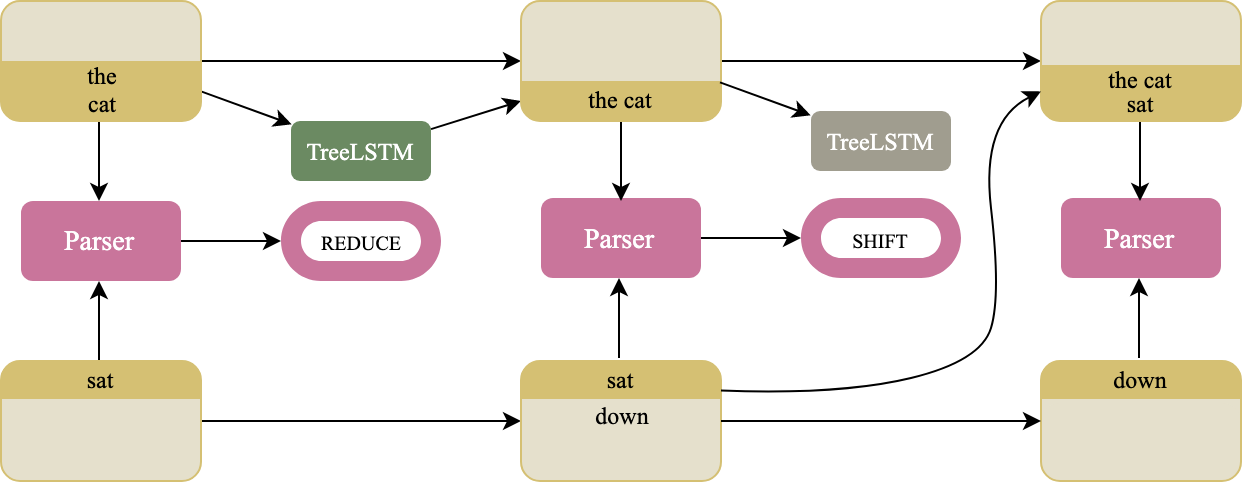
\includegraphics[width=0.8\textwidth]{img/spinnLatentTutorial.png}
\end{figure}
\end{frame}%


\begin{frame}%
\frametitle{\underline{S}tack-augmented \underline{P}arser-\underline{I}nterpreter \underline{N}eural-\underline{N}etwork}%
{\cornercite{bowman-spinn}}

\begin{itemize}%
\item Joint learning: Combines a constituency parser and a sentence representation model.
\item<2-> The parser, $f_{\parp}(x)$ is a transition-based \textbf{shift-reduce} parser. It looks at top two elements of stack and top element of the buffer.
\item<3-> \textbf{TreeLSTM} combines top two elements of the stack when the parser choses the {\rmfamily\scshape{reduce}} action.
\end{itemize}%
\end{frame}

\begin{frame}
\frametitle{\underline{S}tack-augmented \underline{P}arser-\underline{I}nterpreter \underline{N}eural-\underline{N}etwork}%
{\cornercite{bowman-spinn}}

\begin{figure}
\only<1>{\vspace{-1cm}\hspace*{1cm}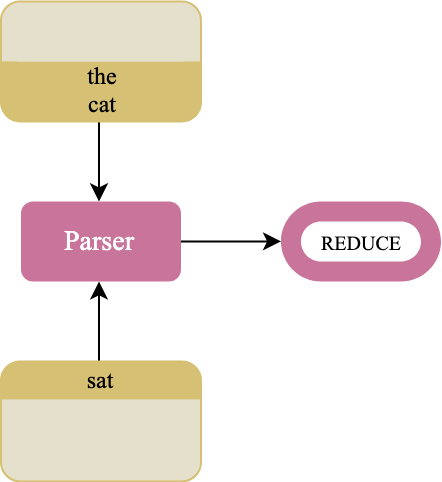
\includegraphics[width=0.3\textwidth,left]{img/200_spinn_1.png}}
\only<2>{\vspace{-1cm}\hspace*{1cm}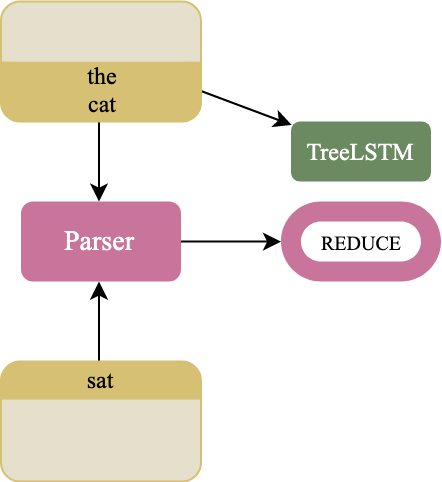
\includegraphics[width=0.3\textwidth,left]{img/200_spinn_2.png}}
\only<3>{\vspace{-1cm}\hspace*{1cm}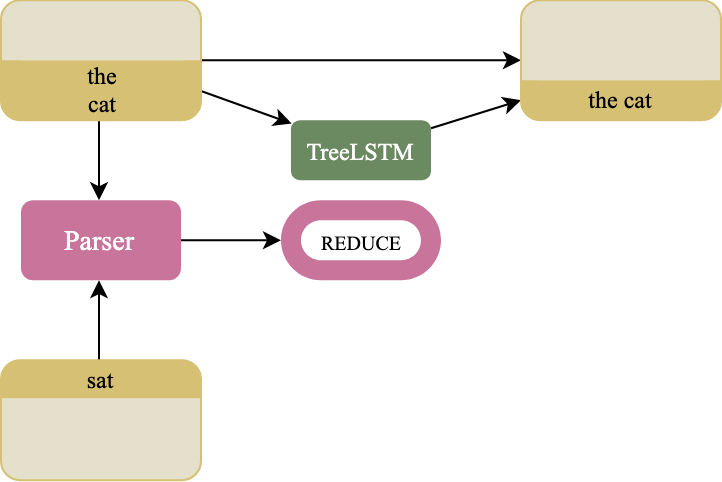
\includegraphics[width=0.5\textwidth,left]{img/200_spinn_3.png}}
\only<4>{\vspace{-1cm}\hspace*{1cm}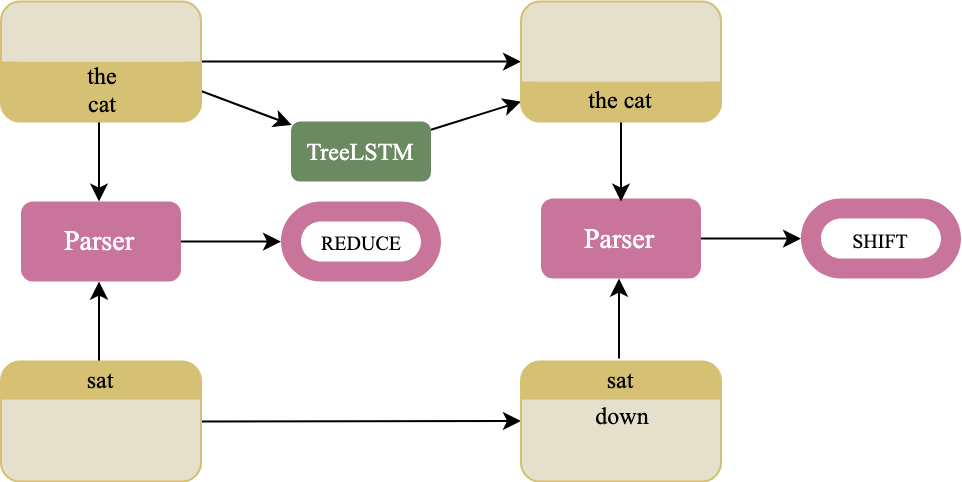
\includegraphics[width=0.65\textwidth,left]{img/200_spinn_4.png}}
\only<5>{\vspace{-1cm}\hspace*{1cm}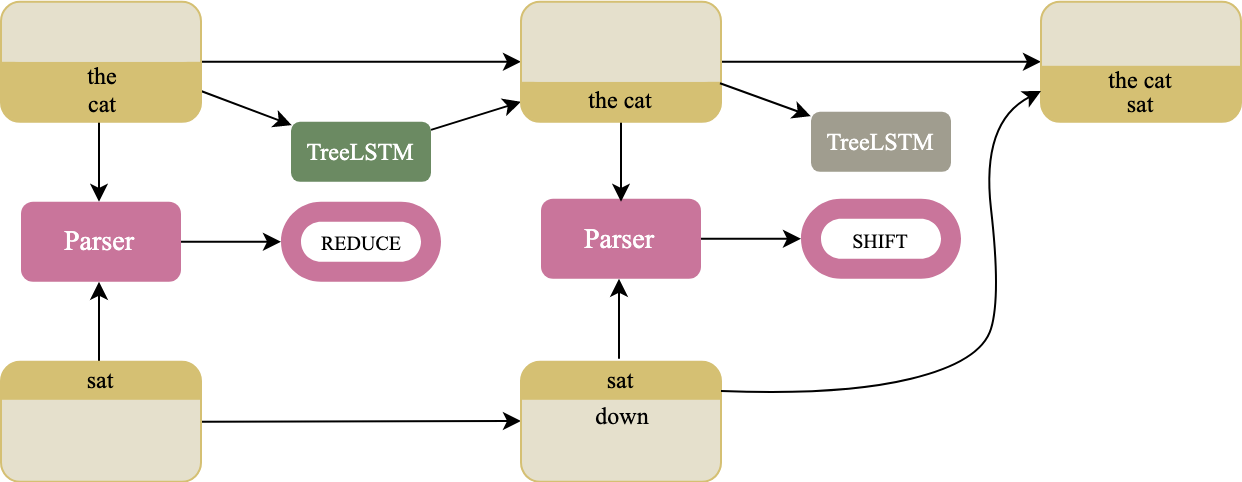
\includegraphics[width=0.8\textwidth,left]{img/200_spinn_5.png}}
\only<6>{\vspace{-1cm}\hspace*{1cm}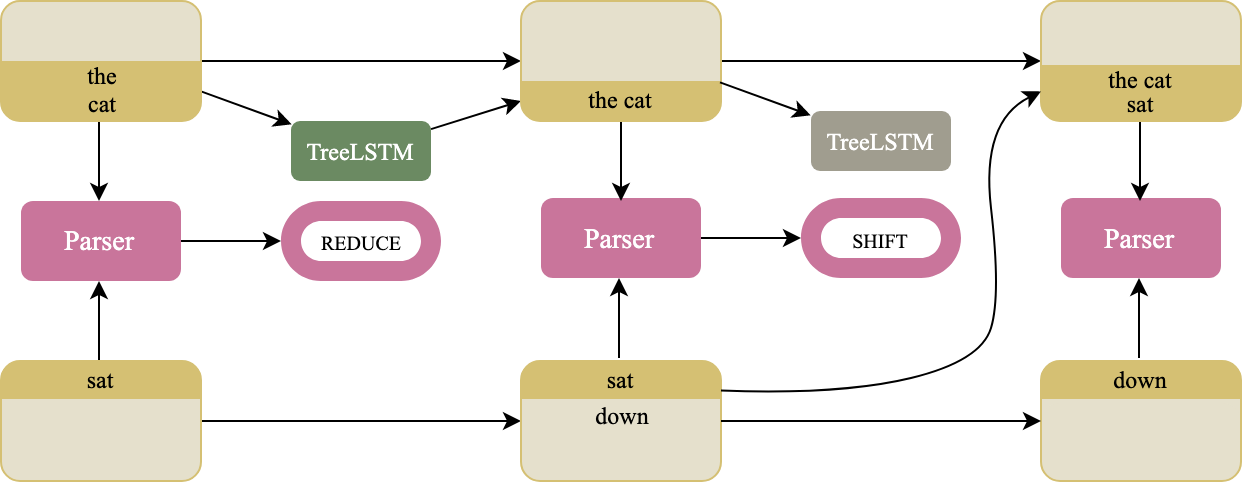
\includegraphics[width=0.8\textwidth,left]{img/spinnLatentTutorial.png}}
\end{figure}
\end{frame}%



%%% SR Math %%%
\begin{frame}
\frametitle{Shift-Reduce parsing}
\begin{itemize}
\item[] We can write a shift-reduce style parse as a sequence of Bernoulli random variables,
$$ \z = \{z_1, \ldots, z_{2L-1}\}$$
\item[] where, $z_j \in \{0,1\} \ \forall j\in[1,2L-1]$
\end{itemize}
\end{frame}

\begin{frame}
\frametitle{Shift-Reduce parsing}
\begin{itemize}
\item[] A sequence of Bernoulli trials but with conditional dependence,
$$p(z_1, z_2, \ldots, z_{2L-1}) = \displaystyle\prod_{j=1}^{2L-1} p(z_j \mid z_{<j})$$
\end{itemize}
\end{frame}




\begin{frame}
\frametitle{Latent structure learning with SPINN}

\begin{itemize}
\item<2-> But now, remove syntactic supervision from SPINN.
\item[] \begin{figure}
\centering
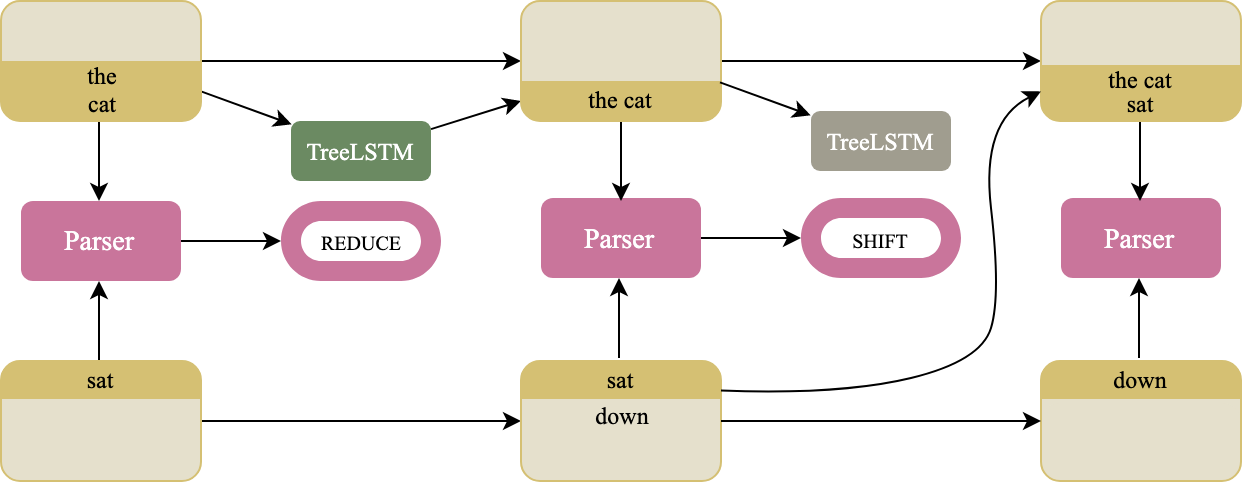
\includegraphics[width=0.6\textwidth]{img/spinnLatentTutorial.png}
\end{figure}
\item<3-> We model the parse, $\z$, as a latent variable with our parser
as the score function estimator, $f_{\parp}(x)$.
\item<4-> With shift-reduce parsing, we're making discrete decisions $\Rightarrow$ REINFORCE as a ``natural" solution.
\end{itemize}

\end{frame}


\sepframe[mygr]{Unsupervised SPINN}


\begin{frame}
\frametitle{Unsupervised SPINN}
\begin{itemize}
	\item[] No syntactic supervision.
	\item[] Only reward is from the downstream task.
	\item[] We only get this reward after parsing the full sentence.
\end{itemize}
\end{frame}

\begin{frame}
\frametitle{SPINN with REINFORCE}
{\cornercite{williams-reinforce}}

Some basic terminology,
\begin{itemize}
\item The \underline{action space} is $z_j\in \{${\rmfamily\scshape{shift}},{\rmfamily\scshape{reduce}}$\}$, and $\z$ is a sequence of actions.
\item<2-> Training parser network parameters, $\parp$ with REINFORCE
\item<3-> The \underline{state}, $\bs{h}$, is the top two elements of the stack and the top element of the buffer.
\item<4-> Learning a \underline{policy network} $\pi(\z \mid \bs{h}; \parp)$
\item<5-> Maximize the \underline{reward}, where $\mathcal{R}$ is performance on the downstream task like sentence classification.
\end{itemize}

\uncover<6>{\overlaybox{NOTE: Only a single reward at the end of parsing.}}

\end{frame}

%%% REINFORCE Algorithm %%%
\begin{frame}%
\frametitle{Through the looking glass of REINFORCE}%
%{\cornercite{williams-reinforce}}

\vspace{-.5\baselineskip}%
\begin{align*}
	\nabla_{\parp} \EE_{\z\sim \parser}[L(\z)] \uncover<2->{&= \nabla_{\parp}
\left[\sum_{\z} L(\z) \parser  \right] \\}
    \uncover<2->{&\small\textit{(By definition of expectation. How to evaluate?)}\\}
    \uncover<3->{&=\sum_{\z} L(\z) \nabla_{\parp} \parser \\}
    %\uncover<3->{&\small\textit{(Not an expectation!)}\\}
    \uncover<4->{&= \sum_{\z} L(\z) \parser \nabla_{\parp} \log \parser \\}
    \uncover<4->{&\small\textit{(By Leibniz integral rule for}\scriptscriptstyle\log\textit{)} \\}
    \uncover<5->{&= \EE_{\z \sim \parser}[L(\z) \nabla_{\parp} \log \parser]}
\end{align*}
\end{frame}




%%% Yogatama %%%
\begin{frame}
\frametitle{SPINN with REINFORCE, aka RL-SPINN}
\begin{itemize}
\item[]\cite{Yogatama2016LearningTC} uses REINFORCE to train SPINN!\\
\item<2->[] However, this vanilla implementation isn't very effective at learning syntax.
\item<3->[] This model fails to solve a simple toy problem.
\end{itemize}
\end{frame}



%%%% LISTOPS %%%%
\begin{frame}
\frametitle{Toy problem: ListOps}%
{\cornercite{nangia-listops}}

\begin{figure}[t]
\centering
\scalebox{1.2}{
\begin{forest}
 shape=coordinate,
 where n children=0{
   tier=word
 }{},
 nice empty nodes
[ [ [ [ [ [\textsc{[max}] [2] ] [9] ] [ [ [ [\textsc{[min}] [4] ] [7] ] [\textsc{]}] ] ] [0] ] [\textsc{]}] ]
\end{forest}
}
%\caption{\label{fig:exampletrees} Example of a parsed ListOps sequence. The parse is left-branching within each list, and each constituent is either a partial list, an integer, or the final closing bracket.}
\end{figure}
\end{frame}


\begin{frame}
\frametitle{Toy problem: ListOps}
{\cornercite{nangia-listops}}

\makebox[0.95\textwidth][c] {% two boxes
\begin{minipage}[t][][c]{.45\textwidth}

\begin{table}[t!]\small
\small \centering
\begin{tabular}{lcccc}
\toprule
 & \multicolumn{2}{c}{\bf Accuracy} & \bf Self  \\
\bf Model & \pmb{$\mu (\sigma)$} & \bf max & \bf F1 \\
\midrule
LSTM & 71.5 (1.5) & \bf 74.4 & - \\
RL-SPINN & 60.7 (2.6) & 64.8 & 30.8 \\
\midrule
Random Trees & - & - & 30.1\\
\bottomrule
\end{tabular}
%\caption{\label{tab:var} \textit{Accuracy} shows accuracy across four runs of the models (expressed as mean, standard deviation, and maximum). \textit{Self F1} shows how well each of these four model runs agrees in its parsing decisions with the other three.}
\end{table}

\end{minipage}%
\hfill%
%
%
\begin{minipage}[t][][c]{.5\textwidth}
\vspace{2.5cm}
\begin{table}[t!]
\small \centering
\begin{tabular}{lcccc}
\toprule
 & \multicolumn{3}{c}{\bf F1 wrt.} & \bf Avg.  \\
\bf Model & \bf LB & \bf RB & \bf GT & \bf Depth  \\
\midrule
48D~~ RL-SPINN &\bf  64.5 & \bf 16.0 & 32.1 & \bf 14.6 \\
128D RL-SPINN & 43.5 & 13.0 & \bf 71.1 & 10.4 \\
%\midrule
%48D~~ ST-Gumbel & 52.2 & 15.3 & 55.3 & 11.1 \\
%128D ST-Gumbel & 56.5 & 9.8 & 57.3 & 12.7 \\
\midrule
GT Trees & 41.6 & 8.8 & 100.0 & 9.6 \\
Random Trees & 24.0 & 24.0 & 24.2 & 5.2 \\
\bottomrule
\end{tabular}
%\caption{\label{tab:f1} \textit{F1 wrt.} shows F1 scores on ListOps with respect to left-branching (LB), right-branching (RB), and ground-truth (GT) trees. \textit{Avg. Depth} shows the average across sentences of the average depth of each token in its tree.}
\end{table}

\end{minipage}}

\uncover<2>{\overlaybox{But why?}}

\end{frame}




%%%% PROBLEMS %%%%
\begin{frame}
\frametitle{RL-SPINN's Troubles}
\begin{itemize}
\item[] This system faces at least two big problems,
\begin{itemize}
\item<2->[] {\large 1. High variance of gradients}
\item<2->[] {\large 2. Coadaptation}
\end{itemize}
\end{itemize}
\end{frame}


%%%% VARIANCE %%%%
\begin{frame}
\frametitle{High variance}

\begin{itemize}
\item We have a single reward at the end of parsing.
\item<2-> We are sampling parses from very large search space!\\ \textbf{Catalan number} of binary trees.
\only<3>{
	\begin{align*}
		3 \text{ tokens } &\Rightarrow 5 \text{ trees} \\
		5 \text{ tokens } &\Rightarrow 42 \text{ trees} \\
		10 \text{ tokens } &\Rightarrow 16796 \text{ trees}
	\end{align*}
}
\item<4-> And the policy is stochastic.
\end{itemize}
\end{frame}


\begin{frame}
\frametitle{High variance}

\begin{itemize}
\item[]<1>{So, sometimes the policy lands in a ``rewarding state":}\\
\end{itemize}

\only<1>{\begin{figure}[t]
\centering
	\scalebox{1.0}{
	\begin{forest}
		shape=coordinate,
		where n children=0{
			tier=word
		}{},
		nice empty nodes
		[ [ [ [ [ [\textsc{[sm}] [\textsc{[sm}] ] [\textsc{[sm}] ] [ [ [\textsc{[max}] [ [5] [ [6] [\textsc{]}] ] ] ] [ [2] [\textsc{]}] ] ] ] [ [0] [ [\textsc{]}] [ [5] [ [0] [8] ] ] ] ] ] [ [6] [\textsc{]}] ] ]
	\end{forest}
}
\caption{Truth: 7; Pred: 7}
\end{figure}
}

\begin{itemize}
\item[]<2>{Sometimes it doesn't:}
\end{itemize}

\only<2>{\begin{figure}[t]
\centering
	\scalebox{1.0}{
	\begin{forest}
		shape=coordinate,
		where n children=0{
			tier=word
		}{},
		nice empty nodes
		[ [ [ [ [ [ [ [ [ [ [ [ [\textsc{[max}] [ [\textsc{[med}] [ [\textsc{[med}] [1] ] ] ] [\textsc{[sm}] ] [3] ] [1] ] [3] ] [\textsc{]}] ] [9] ] [\textsc{]}] ] [6] ] [\textsc{]}] ] [5] ] [\textsc{]}] ]
	\end{forest}
}
\caption{Truth: 6; Pred: 5}
\end{figure}
}

\end{frame}


\begin{frame}
\frametitle{High variance}
\begin{itemize}
\item[] \textbf{Catalan number} of parses means we need many many samples to lower variance!
\item<2->[] Possible solutions,
\begin{itemize}
\item[] 1. Gradient normalization
\item[] 2. Control variates, aka baselines
\end{itemize}
\end{itemize}
\end{frame}


%%% CONTROL VARIATES %%%
\begin{frame}
\frametitle{Control variates}
\begin{itemize}
\item A simple control variate: moving average of recent rewards
\item<2-> Parameters are updated using the \underline{advantage} which is the difference between the reward, $\mathcal{R}$, and the baseline prediction.
\item[]<3-> So,
\begin{align*}
	\nabla \EE_{\z\sim\pi(\z)} = \EE_{\z\sim \pi(\z)}[\left(\textcolor{tBleu}{L(\z)} - \textcolor{tPink}{b(\bs{x})}\right) \nabla \pi(\z)]
\end{align*}
\item[]<4->Which we can do because,
\begin{align*}
	\sum_z \textcolor{tPink}{b(\bs{x})} \nabla\pi(\z) = \textcolor{tPink}{b(\bs{x})}\sum_z\nabla\pi(\z) = \textcolor{tPink}{b(\bs{x})} \nabla 1 = 0
\end{align*}
\end{itemize}
\end{frame}


%%%% PROBLEMS %%%%
\begin{frame}
\frametitle{Issues with SPINN with REINFORCE}
\begin{itemize}
\item[] This system faces two big problems,
\begin{itemize}
\item[] {\large 1. High variance of gradients}
\item[] {\large 2. Coadaptation}
\end{itemize}
\end{itemize}
\end{frame}


%%% COADAPTATION %%%
\begin{frame}
\frametitle{Coadaptation problem}
\begin{itemize}
\item[] Learning composition function parameters $\clfp$ with backpropagation,
\item[] and parser parameters $\parp$ with REINFORCE.
\item<2->[]
\item<2->[] Generally, $\clfp$ will be learned more quickly than $\parp$,
 \item<2->[] making it harder to explore the parsing search space and optimize for $\parp$.
\item<3->[]
\item<3->[] Difference in variance of two gradient estimates.
\end{itemize}
\uncover<4>{\overlaybox{Possible solution:\\ Proximal Policy Optimization (Schulman et al., 2017)}}
\end{frame}


\begin{frame}
\frametitle{Making REINFORCE+SPINN work}
\begin{itemize}
\item[] \cite{havrylov-2019-cooperative} use,
	\begin{itemize}
		\item[] 1. Input dependent control variate
		\item[] 2. Gradient normalization
		\item[] 3. Proximal Policy Optimization
	\end{itemize}
\item<2->[]
\item<2->[] They solve ListOps!
\item<3->[] However, does not learn English grammars.
\end{itemize}
\end{frame}



\begin{frame}%
\frametitle{Should I? Shouldn't I?}%
\makebox[\textwidth][c] {% two boxes
\begin{minipage}[t][][c]{.45\textwidth}
\begin{itemize}
\item Unbiased!
\item<3-> In a simple setting, with enough tricks, it can work! \emoji{happ}
\end{itemize}
\end{minipage}

\begin{minipage}[t][][c]{.45\textwidth}
\begin{itemize}
\item<2-> High variance \emoji{frown}
\item<4-> Has not yet been very effective at learning English syntax.
\end{itemize}
\end{minipage}

}
\end{frame}

\section{Gradient surrogates}
\sepframe{III. Gradient Surrogates}

\begin{frame}
\centering
So far:
\begin{itemize}
    \item Tackled \textbf{expected loss} in a \textbf{stochastic
        computation graph}
        $$ \EE_{\parser} \big[ L(\z) \big] $$
    \item<2-> Optimized with the \textbf{REINFORCE} estimator.
    \item<3-> Struggled with variance \& sampling.
\end{itemize}
\vspace{\baselineskip}
\uncover<4->{In this section:}
\begin{itemize}
    \item<4-> Consider the \textbf{deterministic alternative}:\\
        \uncover<5->{
\parbox{.333\textwidth}{\quad pick ``best'' structure}%
\parbox{.333\textwidth}{\hfil$\hat{\z}(x) \defeq \argmax_{\z \in
\mathcal{M}} \parser $\hfil}
\parbox{.333\textwidth}{}%
}
        \uncover<6->{

\parbox{.333\textwidth}{\quad incur loss}%
\parbox{.333\textwidth}{\hfil$L\big(\hat{\z}(x)\big)$\hfil}%
\parbox{.333\textwidth}{}%
}
    \item<7-> 3A: try to optimize the deterministic loss directly
    \item<8-> 3B: use this strategy to reduce variance in the stochastic model.
\end{itemize}
\end{frame}

\begin{frame}%
\frametitle{Recap: The argmax problem}
\centering%
\begin{tikzpicture}%
%
\drawcs\drawscores\drawargmax[\z]
%
\node at (0, -1) {$\frac{\partial \z}{\partial \s}=\bs{0}$};
\node[anchor=south,align=center] at (-6, \vecheight*2+1) (in) {\phantom{input}};
\node[anchor=south,align=center] at (6, \vecheight*2+1) (out) {\phantom{output}};
\end{tikzpicture}%
\\[-\baselineskip]

\begin{tikzpicture}[overlay]
    \draw[axisline,->] (3, 3) -- (3, 6) node[left] {$\zz_1$};
    \draw[axisline,->] (3, 3) -- (7, 3) node[right]{$\ss_1$};

    \node[axislabel,left] at (3, 3) {$0$};
    \node[axislabel,left] at (3, 5) {$1$};

    \draw[axisline] ($(3,3) + (-\ticksize, 0)$) -- ($(3,3) + (+\ticksize, 0)$);
    \draw[axisline] ($(3,4) + (-\ticksize, 0)$) -- ($(3,4) + (+\ticksize, 0)$);
    \draw[axisline] ($(3,5) + (-\ticksize, 0)$) -- ($(3,5) + (+\ticksize, 0)$);

    \draw[axisline] ($(3,3) + (0, -\ticksize)$) -- ($(3,3) + (0, +\ticksize)$);
    \draw[axisline] ($(4,3) + (0, -\ticksize)$) -- ($(4,3) + (0, +\ticksize)$);
    \draw[axisline] ($(5,3) + (0, -\ticksize)$) -- ($(5,3) + (0, +\ticksize)$);
    \draw[axisline] ($(6,3) + (0, -\ticksize)$) -- ($(6,3) + (0, +\ticksize)$);

    \node[axislabel,below] at (4, 3) {$\ss_2 - 1$};
    \node[axislabel,below] at (5, 3) {$\ss_2$};
    \node[axislabel,below] at (6, 3) {$\ss_2 + 1$};

    \draw[ultra thick,colorArgmax] (3, 3) -- (5,3) ;
    \draw[ultra thick,colorArgmax] (5, 5) -- (7,5) ;

    \node[anchor=south,align=center] at (-5, 4) (in) {$\z = \argmax(\s)$};
\end{tikzpicture}\end{frame}


\begin{frame}%
\frametitle{Softmax}
\centering%
\begin{tikzpicture}%
%
\drawcs\drawscores\drawsoftmax
\node at (0, -1) {$\frac{\partial \p}{\partial \s}=\operatorname{diag}(\p) - \p\p^\top$};
\node[anchor=south,align=center] at (-6, \vecheight*2+1) (in) {\phantom{input}};
\node[anchor=south,align=center] at (6, \vecheight*2+1) (out) {\phantom{output}};
\end{tikzpicture}
\\[-\baselineskip]

\begin{tikzpicture}[overlay]
    \draw[axisline,->] (3, 3) -- (3, 6) node[left] {$\pp_1$};
    \draw[axisline,->] (3, 3) -- (7, 3) node[right]{$\ss_1$};

    \node[axislabel,left] at (3, 3) {$0$};
    \node[axislabel,left] at (3, 5) {$1$};

    \draw[axisline] ($(3,3) + (-\ticksize, 0)$) -- ($(3,3) + (+\ticksize, 0)$);
    \draw[axisline] ($(3,4) + (-\ticksize, 0)$) -- ($(3,4) + (+\ticksize, 0)$);
    \draw[axisline] ($(3,5) + (-\ticksize, 0)$) -- ($(3,5) + (+\ticksize, 0)$);

    \draw[axisline] ($(3,3) + (0, -\ticksize)$) -- ($(3,3) + (0, +\ticksize)$);
    \draw[axisline] ($(4,3) + (0, -\ticksize)$) -- ($(4,3) + (0, +\ticksize)$);
    \draw[axisline] ($(5,3) + (0, -\ticksize)$) -- ($(5,3) + (0, +\ticksize)$);
    \draw[axisline] ($(6,3) + (0, -\ticksize)$) -- ($(6,3) + (0, +\ticksize)$);

    \node[axislabel,below] at (4, 3) {$\ss_2 - 1$};
    \node[axislabel,below] at (5, 3) {$\ss_2$};
    \node[axislabel,below] at (6, 3) {$\ss_2 + 1$};

    \draw[ultra thick,colorArgmax] (3, 3) -- (5,3) ;
    \draw[ultra thick,colorArgmax] (5, 5) -- (7,5) ;

    \draw (3, 3.1) edge[colorSoftmax,ultra thick,out=360,in=180,looseness=1.5] (7, 4.9);

    \node[anchor=south,align=center] at (-5, 4) (in) {$\pp_j = \exp(\ss_j) / Z$};

\end{tikzpicture}%
\end{frame}



\begin{frame}%
\frametitle{Straight-Through Estimator}%
\cornercite{hinton2012ste,bengio2013ste}%
\makebox[\textwidth][c] {% two boxes
\begin{minipage}[t][][c]{.66\textwidth}
\begin{itemize}%
\item<2-> \underline{Forward}: $\z=\argmax(\s)$
\item<4-> \underline{Backward}:
pretend $\z$ was some continuous $\tilde\p$; $\pfrac{\tilde{\p}}{\s}\neq \bs{0}$
\begin{itemize}
\item<6-> simplest: identity, $\tilde\p(\s)=\s, \pfrac{\tilde \p}{\s}=\bs{I}$
\item<7-> others, e.g.\ softmax $\tilde\p(\s) = \softmax(\s), \pfrac{\tilde\p}{\s}=\diag(\tilde\p) - \tilde\p\tilde\p^\top$
\end{itemize}%
\item<8-> More explanation in a while

\end{itemize}%
\end{minipage}%
% \hfill%
%
\begin{minipage}[t][][c]{.33\textwidth}
\centering
\begin{tikzpicture}
{
\node[anchor=south] at (-.3-.5*\vecwidth, \vecheight*5+.3) {$\s$};
\draw[elem,fill=vecfg!60!vecbg] (-1-\vecwidth, \vecheight*4+1) rectangle (-1, \vecheight*5+1);
\draw[elem,fill=vecfg!85!vecbg] (-1-\vecwidth, \vecheight*3+1) rectangle (-1, \vecheight*4+1);
\draw[elem,fill=vecfg!60!vecbg] (-1-\vecwidth, \vecheight*2+1) rectangle (-1, \vecheight*3+1);
\draw[elem,fill=vecfg!75!vecbg] (-1-\vecwidth, \vecheight*1+1) rectangle (-1, \vecheight*2+1);
\draw[elem,fill=vecfg!50!vecbg] (-1-\vecwidth, \vecheight*0+1) rectangle (-1, \vecheight*1+1);
}(nodetilde)

% {}
\uncover<2->{
\def\vecwidth{.5}
\def\vecheight{.5}
% \drawargmax
{
\node[anchor=south] at (1.5+.5*\vecwidth, \vecheight*9.6) {$\z$};
\draw[elem,fill=vecfg! 0!vecbg]  (1, \vecheight*4+3) rectangle (1+\vecwidth, \vecheight*5+3);
\draw[elem,fill=vecfg!70!vecbg]  (1, \vecheight*3+3) rectangle (1+\vecwidth, \vecheight*4+3);
\draw[elem,fill=vecfg! 0!vecbg]  (1, \vecheight*2+3) rectangle (1+\vecwidth, \vecheight*3+3);
\draw[elem,fill=vecfg! 0!vecbg]  (1, \vecheight*1+3) rectangle (1+\vecwidth, \vecheight*2+3);
\draw[elem,fill=vecfg! 0!vecbg]  (1, \vecheight*0+3) rectangle (1+\vecwidth, \vecheight*1+3);
}
}
\uncover<3->{
% Arrows forward
\draw[->][very thick, color=mygr](-2*\vecheight,6*\vecheight) -- (2*\vecheight,8.5*\vecheight);
\draw[->][very thick, color=mygr](3*\vecheight,8.5*\vecheight) -- (5*\vecheight,8.5*\vecheight);
\draw[->][very thick, color=mygr](-5*\vecheight,6*\vecheight) -- (-3.5*\vecheight,6*\vecheight);
}
\uncover<4->{
\node[anchor=south] at (1.5+.5*\vecwidth, \vecheight*5-0.8) {$\tilde \p$};
\draw[elem,fill=vecfg!30!vecbg]  (1, \vecheight*4) rectangle (1+\vecwidth, \vecheight*5);
\draw[elem,fill=vecfg!50!vecbg]  (1, \vecheight*3) rectangle (1+\vecwidth, \vecheight*4);
\draw[elem,fill=vecfg!35!vecbg]  (1, \vecheight*2) rectangle (1+\vecwidth, \vecheight*3);
\draw[elem,fill=vecfg!25!vecbg]  (1, \vecheight*1) rectangle (1+\vecwidth, \vecheight*2);
\draw[elem,fill=vecfg!15!vecbg]  (1, \vecheight*0) rectangle (1+\vecwidth, \vecheight*1);
}
\uncover<5->{
% arrows back
\draw[->][tGreen,very thick](2*\vecheight,2.5*\vecheight) -- (-2*\vecheight,5.5*\vecheight);
\draw[->][tGreen,very thick](5*\vecheight,2.5*\vecheight) -- (3*\vecheight,2.5*\vecheight);
\draw[->][tGreen,very thick](-3.5*\vecheight,5.5*\vecheight) -- (-5*\vecheight,5.5*\vecheight);
}

\end{tikzpicture}
\end{minipage}}
\uncover<9>{\overlaybox{What about the structured case?}}
\end{frame}

\againframe{structuretypes}

\begin{frame}%
\frametitle{STE for incremental structures}%
\centering
\begin{itemize}
    \item<2-> Build a structure as a sequence of discrete choices (e.g., shift-reduce)
    \item<3-> Assigns a score to any (partial structure, action) tuple.
    \item<4-> In this case, we just apply the straight-through estimator for each step.
    \item<5-> \underline{Forward}: the \textbf{highest scoring action} for each step
    \item<6-> \underline{Backward}: pretend that we had used a \textbf{differentiable surrogate function}
    \item[]<7-> \underline{Example}: Latent Tree Learning with Differentiable Parsers: Shift-Reduce Parsing and Chart Parsing \citep{maillard2018latent} (STE through beam search).
\end{itemize}
\end{frame}

\begin{frame}
\frametitle{STE for the factorized approach}
Requires a bit more work:
\begin{itemize}
\item Recap: marginal polytope
\item Predicting structures globally: Maximum A Posteriori (MAP)
\item Deriving Straight-Through and SPIGOT
\end{itemize}
\end{frame}

\againframe{marginalpoly}

\begin{frame}
\frametitle{Predicting structures from scores of parts}
% \centering
\begin{columns}[t]%
\begin{column}{.4\textwidth}%
\centering
\begin{itemize}
\item $\eta(i \rightarrow j)$: score of arc $i \rightarrow j$
\item $\zz(i \rightarrow j)$: is arc $i \rightarrow j$ selected?
\item<2-> Task-specific algorithm for the highest-scoring structure.
%\item<3-> Backward: identity $\frac{\partial \tilde\mg}{\partial \pr}=\bs{I}$
\end{itemize}
\end{column}
\begin{column}[T]{.6\textwidth}%
\centering
\begin{tikzpicture}
% \only<3>{\drawcs}
% \only<4->{
\node[anchor=south] at (0, \vecheight*4) {\cartoon[.5]{2/3}};
\node[anchor=south] at (0, \vecheight*2.5) {\cartoon[.5]{1/2}};
%\node[anchor=south] at (0, \vecheight*1.5) {$\cdots$};
\node[anchor=south] at (0, \vecheight*0.5) {\cartoon[.5]{1/4}};
% }
% \only<3->{%
% \drawscores
{\node[anchor=south] at (-1-.5*\vecwidth, \vecheight*5+.1) {$\pr$};
\draw[elem,fill=vecfg!60!vecbg] (-1-\vecwidth, \vecheight*4) rectangle (-1, \vecheight*5);
\draw[elem,fill=vecfg!85!vecbg] (-1-\vecwidth, \vecheight*3) rectangle (-1, \vecheight*4);
\draw[elem,fill=vecfg!60!vecbg] (-1-\vecwidth, \vecheight*2) rectangle (-1, \vecheight*3);
\draw[elem,fill=vecfg!75!vecbg] (-1-\vecwidth, \vecheight*1) rectangle (-1, \vecheight*2);
\draw[elem,fill=vecfg!50!vecbg] (-1-\vecwidth, \vecheight*0) rectangle (-1, \vecheight*1);
}
% \drawargmax
{\node[anchor=south] at (1+.5*\vecwidth, \vecheight*5+.1) {$\z$};
\draw[elem,fill=vecfg! 0!vecbg]  (1, \vecheight*4) rectangle (1+\vecwidth, \vecheight*5);
\draw[elem,fill=vecfg!70!vecbg]  (1, \vecheight*3) rectangle (1+\vecwidth, \vecheight*4);
\draw[elem,fill=vecfg! 0!vecbg]  (1, \vecheight*2) rectangle (1+\vecwidth, \vecheight*3);
\draw[elem,fill=vecfg!70!vecbg]  (1, \vecheight*1) rectangle (1+\vecwidth, \vecheight*2);
\draw[elem,fill=vecfg! 0!vecbg]  (1, \vecheight*0) rectangle (1+\vecwidth, \vecheight*1);
}


% \node[anchor=south] at (-2, \vecheight*3+1) (in-end) {};
\node[anchor=south,align=center] at (6, \vecheight*3+1)
(out){output\\$\widetilde{\bs{y}}$};
% \node[anchor=south] at (2, \vecheight*3+1) (out-end) {};
% \path (in) edge[->,very thick,bend right=50] (in-end);
\node[anchor=south] at (4, \vecheight*3+.9) (out-mid) {
    {\cartoon[.9]{1/2,1/4}}
};
\path (out-end) edge[->,very thick,bend right=50] (out-mid.south west);
\path (out-mid.south east) edge[->,very thick,bend right=50] (out);
% }
\end{tikzpicture}
\end{column}
\end{columns}
\end{frame}

\begin{frame}<1>[label=algos]
\frametitle{Algorithms for specific structures}
\fontsize{10pt}{11}\selectfont%
\centering%
\renewcommand{\arraystretch}{3}%
\begin{tabular}{l c <{\onslide<2->}c<{\onslide}}
&\textbf{Best structure (MAP)} & \textbf{Marginals} \\
\tikzmark{seq}%
\textbf{Sequence tagging}
& \makecell{Viterbi \\ \citep{Rabiner1989}}
& \makecell{Forward-Backward \\ \citep{Rabiner1989}}
\\
%
\textbf{Constituent trees}
& \makecell{CKY \\ \citep{kasami,younger} \\ \citep{cocke}}
& \makecell{Inside-Outside\\\citep{insideoutside}}%
\\
\tikzmark{alig}%
\textbf{Temporal alignments}
& \makecell{DTW \\ \citep{dtw}}
& \makecell{Soft-DTW \\ \citep{softdtw}}
\\
\textbf{Dependency trees}
& \makecell{Max. Spanning Arborescence \\ \citep{Chu1965,Edmonds1967}}
& \makecell{Matrix-Tree \\ \citep{Kirchhoff1847}}
\\
%
\textbf{Assignments}
& \makecell{Kuhn-Munkres \\ \citep{hungarian,lapjv}}
& \makecell{\alert{\#P-complete} \\ \citep{valiant,taskar-thesis}} \\
\end{tabular}
\begin{tikzpicture}[%
    remember picture,
    overlay]
    \draw<3->[decorate,decoration={brace,amplitude=5pt}] ([xshift=-1.5ex]pic cs:alig)
         -- ([xshift=-1.5ex]pic cs:seq)
         node [midway,xshift=-15pt,align=center] {dyn.\\prog.};
\end{tikzpicture}
\end{frame}


\begin{frame}[t]
\frametitle{Structured Straight-Through}
\makebox[\textwidth][c] {% two boxes
\begin{minipage}[t][][c]{.5\textwidth}
\begin{itemize}
\item Forward pass:
\\ \quad Find highest-scoring structure:
\\ \quad $\z = \displaystyle\argmax_{\z\in\ZZ} \pr^\top \z$
\item Backward pass:
\\ \quad pretend we used $\tilde\mg = \pr$.
\end{itemize}
\end{minipage}%
\begin{minipage}[t][][c]{.5\textwidth}
\centering
\begin{tikzpicture}
{
\node[anchor=south] at (-.3-.5*\vecwidth, \vecheight*5+.3) {$\pr$};
\draw[elem,fill=vecfg!60!vecbg] (-1-\vecwidth, \vecheight*4+1) rectangle (-1, \vecheight*5+1);
\draw[elem,fill=vecfg!85!vecbg] (-1-\vecwidth, \vecheight*3+1) rectangle (-1, \vecheight*4+1);
\draw[elem,fill=vecfg!60!vecbg] (-1-\vecwidth, \vecheight*2+1) rectangle (-1, \vecheight*3+1);
\draw[elem,fill=vecfg!75!vecbg] (-1-\vecwidth, \vecheight*1+1) rectangle (-1, \vecheight*2+1);
\draw[elem,fill=vecfg!50!vecbg] (-1-\vecwidth, \vecheight*0+1) rectangle (-1, \vecheight*1+1);
}(nodetilde)

\def\vecwidth{.5}
\def\vecheight{.5}
% \drawargmax
{
\node[anchor=south] at (1.5+.5*\vecwidth, \vecheight*9.6) {$\z$};
\draw[elem,fill=vecfg! 0!vecbg]  (1, \vecheight*4+3) rectangle (1+\vecwidth, \vecheight*5+3);
\draw[elem,fill=vecfg!70!vecbg]  (1, \vecheight*3+3) rectangle (1+\vecwidth, \vecheight*4+3);
\draw[elem,fill=vecfg! 0!vecbg]  (1, \vecheight*2+3) rectangle (1+\vecwidth, \vecheight*3+3);
\draw[elem,fill=vecfg! 0!vecbg]  (1, \vecheight*1+3) rectangle (1+\vecwidth, \vecheight*2+3);
\draw[elem,fill=vecfg!70!vecbg]  (1, \vecheight*0+3) rectangle (1+\vecwidth, \vecheight*1+3);
}
% Arrows forward
\draw[->][very thick, color=mygr](-2*\vecheight,6*\vecheight) -- (2*\vecheight,8.5*\vecheight);
\draw[->][very thick, color=mygr](3*\vecheight,8.5*\vecheight) -- (5*\vecheight,8.5*\vecheight);
\draw[->][very thick, color=mygr](-5*\vecheight,6*\vecheight) -- (-3.5*\vecheight,6*\vecheight);
\node[anchor=south] at (1.5+.5*\vecwidth, \vecheight*5-0.8) {$\tilde \mg$};
\draw[elem,fill=vecfg!60!vecbg]  (1, \vecheight*4) rectangle (1+\vecwidth, \vecheight*5);
\draw[elem,fill=vecfg!85!vecbg]  (1, \vecheight*3) rectangle (1+\vecwidth, \vecheight*4);
\draw[elem,fill=vecfg!60!vecbg]  (1, \vecheight*2) rectangle (1+\vecwidth, \vecheight*3);
\draw[elem,fill=vecfg!75!vecbg]  (1, \vecheight*1) rectangle (1+\vecwidth, \vecheight*2);
\draw[elem,fill=vecfg!50!vecbg]  (1, \vecheight*0) rectangle (1+\vecwidth, \vecheight*1);
% arrows back
\draw[->][tGreen,very thick](2*\vecheight,2.5*\vecheight) -- (-2*\vecheight,5.5*\vecheight);
\draw[->][tGreen,very thick](5*\vecheight,2.5*\vecheight) -- (3*\vecheight,2.5*\vecheight);
\draw[->][tGreen,very thick](-3.5*\vecheight,5.5*\vecheight) -- (-5*\vecheight,5.5*\vecheight);
\end{tikzpicture}
\end{minipage}}
\end{frame}



\begin{frame}
\frametitle{Straight-Through Estimator}
\framesubtitle{Revisited}
\begin{itemize}
\item<2-> In the forward pass, $\z = \argmax(\s)$.
\item<3-> if we had labels (multi-task learning),
$L_\text{MTL} = \textcolor{tBleu}{L\big(\hat{y}(\z), y\big)} \textcolor{tGreen}{+
L_\text{hid}(\s,\z^\text{true})}$
\item<4-> One choice: perceptron loss
\textcolor{tGreen}{$L_\text{hid}(\s,\z^\text{true}) = \s^\top\z - \s^\top
\z^\text{true};
\quad
\pfrac{L_\text{hid}}{\s} = \z - \z^\text{true}
$}.
\item<5-> We don't have labels! Induce labels by ``pulling back'' the downstream
target:
\\ \quad the ``best'' (unconstrained) latent value would be:\quad
$\argmin_{\tilde{\z}\in\mathbb{R}^D} L\big(\hat{y}(\tilde{\z}), y\big)$
\item<6-> One gradient descent step starting from $\z$: $\z^\text{true} \leftarrow
\z -  \pfrac{L}{\z}$
\item[]<7->% perceptron loss yields:
$$
\pfrac{L_\text{MTL}}{\s} =
\textcolor{tBleu}{\underbrace{\pfrac{L}{\s}}_{=\bs{0}}} +
\textcolor{tGreen}{\pfrac{L_\text{hid}}{\s}}
\uncover<8->{%
= \textcolor{tGreen}{\z - \left(\z -
\pfrac{L}{\z}
\right)
} =
\pfrac{L}{\z}
}
$$
\end{itemize}%
\cornercite{stspigotnote}%
\end{frame}


\begin{frame}%
\frametitle{Straight-Through in the structured case}%
\cornercite{peng2018backpropagating,stspigotnote}
% \centering
\begin{columns}[t]
\begin{column}{.65\textwidth}
\begin{itemize}
\small
\item<1-> Structured STE: perceptron update with induced annotation
\small
$$\argmin_{\mg \in \reals^D}
L(\hat{y}(\mg), y)
\quad\quad
\approx \z - \nabla_{\z} L(\z)
\rightarrow \z^\text{true}
$$ \\
{\small (one step of gradient descent)}
\item<2-> SPIGOT takes into account the constraints; uses the induced annotation
$$\argmin_{\mg \textcolor{tPink}{\in
\mathcal{M}}}
L(\hat{y}(\mg), y)
\quad
\approx \operatorname{Proj}_\mathcal{M} \big(\z -
\nabla_{\z} L(\z) \big)
\rightarrow \z^\text{true}
$$ \\
{\small (one step of \emph{projected} gradient descent!)}
\item<3-> We discuss a generic way to compute the projection in part 4.
\end{itemize}
\end{column}
\begin{column}[T]{.35\textwidth}
\begin{itemize}
    \item[]<1-> 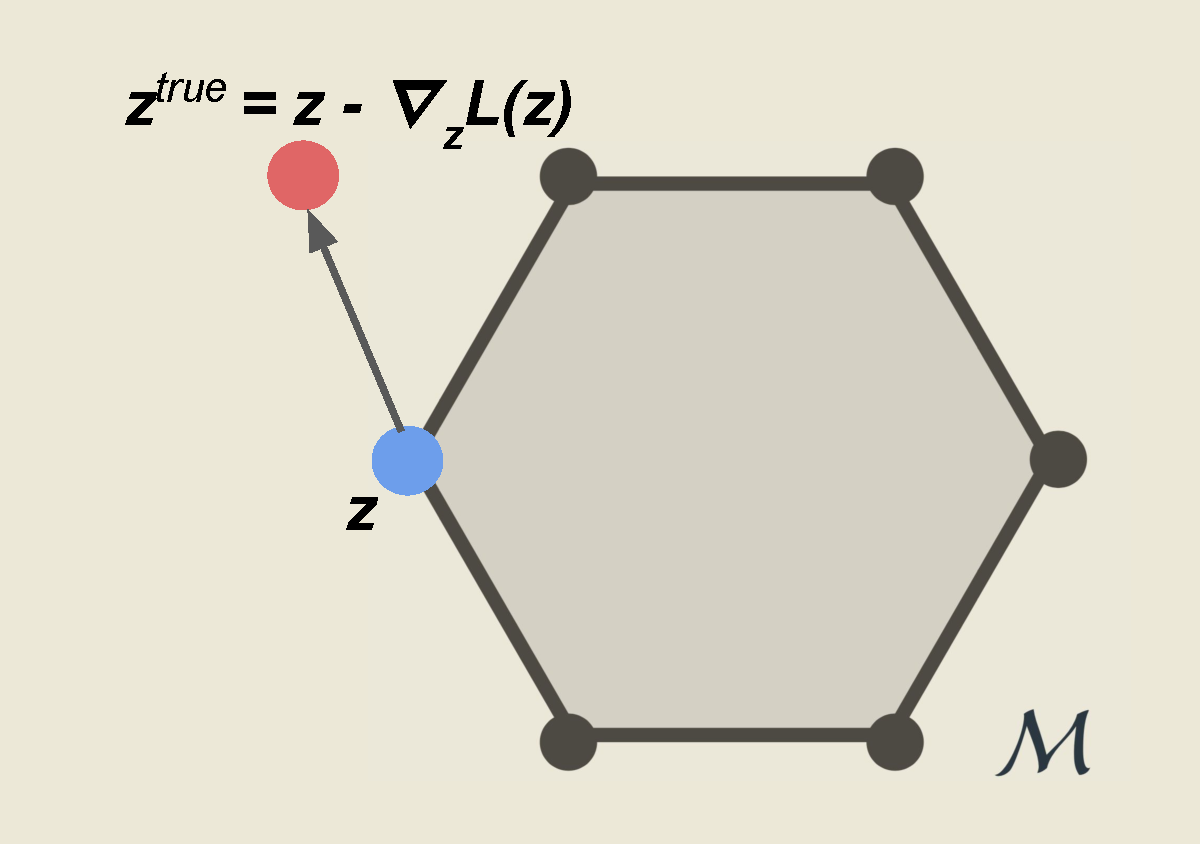
\includegraphics[width=0.8\textwidth]{img/300_spigot_ste.pdf}
    \item[]<2-> 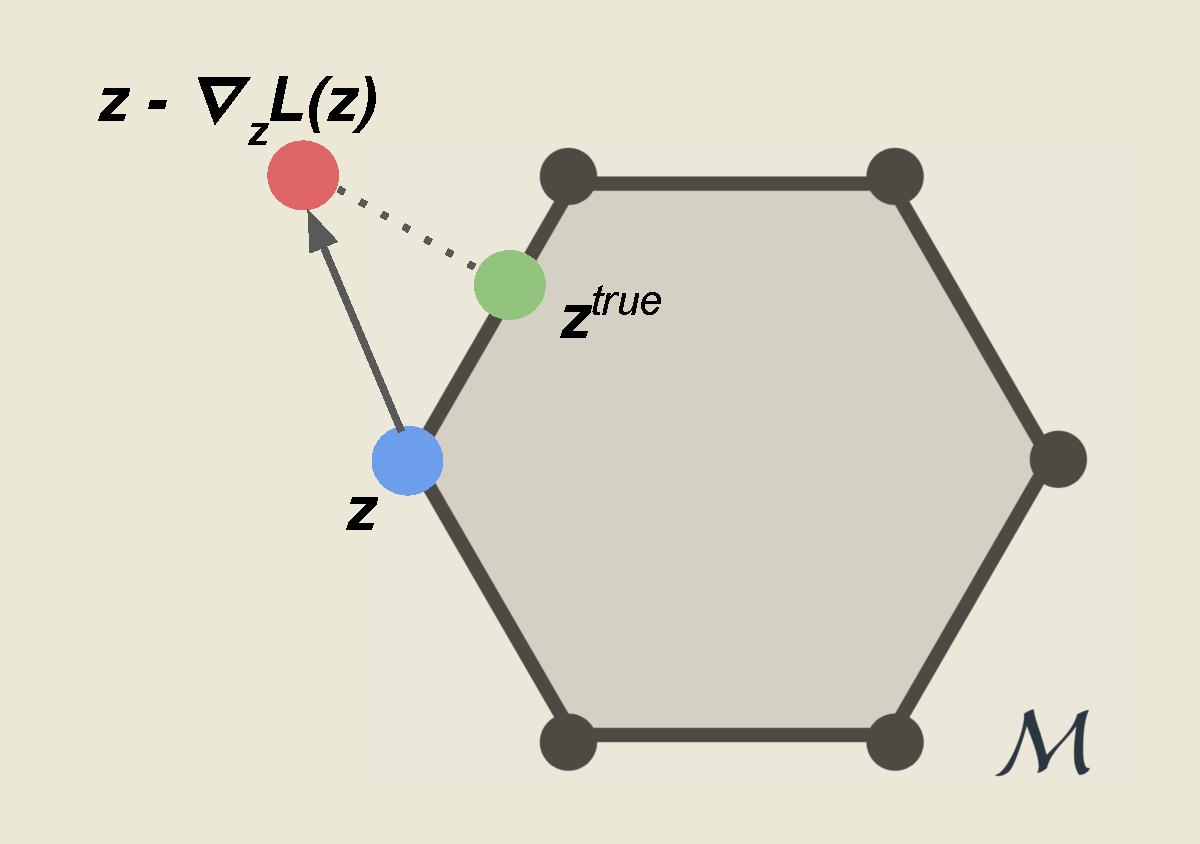
\includegraphics[width=0.8\textwidth]{img/300_spigot_update.pdf}
\end{itemize}
\end{column}
\end{columns}
\end{frame}


\begin{frame}%
\frametitle{Summary: Straight-Through Estimator}%
\centering
\begin{itemize}
    \item[]<2-> We saw how to use the \textit{Straight-Through Estimator} to allow learning models with \textit{argmax} in the middle of the computation graph.\\
    \item[]<3-> We were optimizing
\parbox{.333\textwidth}{\hfil$L\big(\hat{\z}(x)\big)$\hfil}\\

    \item[]<4->
    \smallskip
    Now we will see how to apply STE for stochastic graphs, as an alternative approach of REINFORCE.
\end{itemize}
\end{frame}


\begin{frame}%
\frametitle{Stochastic node in the computation graph}%
\centering
\begin{itemize}
    \item[]<2-> Recall the stochastic objective:
        $$ \EE_{\parser} \big[ L(\z) \big] $$
    \item<3-> REINFORCE (previous section).
    \uncover<4->{ High variance. \emoji{frown}}
    \item<5-> An alternative is using the \textit{reparameterization trick} \citep{kingma2013auto}.
\end{itemize}
\end{frame}


\begin{frame}
\frametitle{Categorical reparameterization}%
\uncover<3->{\cornercite{jang2016categorical, maddison2016concrete}}
\centering
\begin{columns}[T]
\begin{column}[T]{.5\textwidth}
\begin{itemize}
    \item<2-> Sampling from a categorical value in the middle of the computation graph.\\
    $\z \sim \parser \propto \exp \bs{s}_{\parp}(\z \mid x)$
    \item<3-> What is the gradient of a sample $\pfrac{\z}{\parp}$?!
    \item<4-> Reparameterization:
    Move the stochasticity out of the gradient path.
    \item<5-> Makes $\z$ deterministic w.r.t.\ $\s$!

\end{itemize}
\end{column}
\begin{column}{.6\textwidth}
\only<2-3>{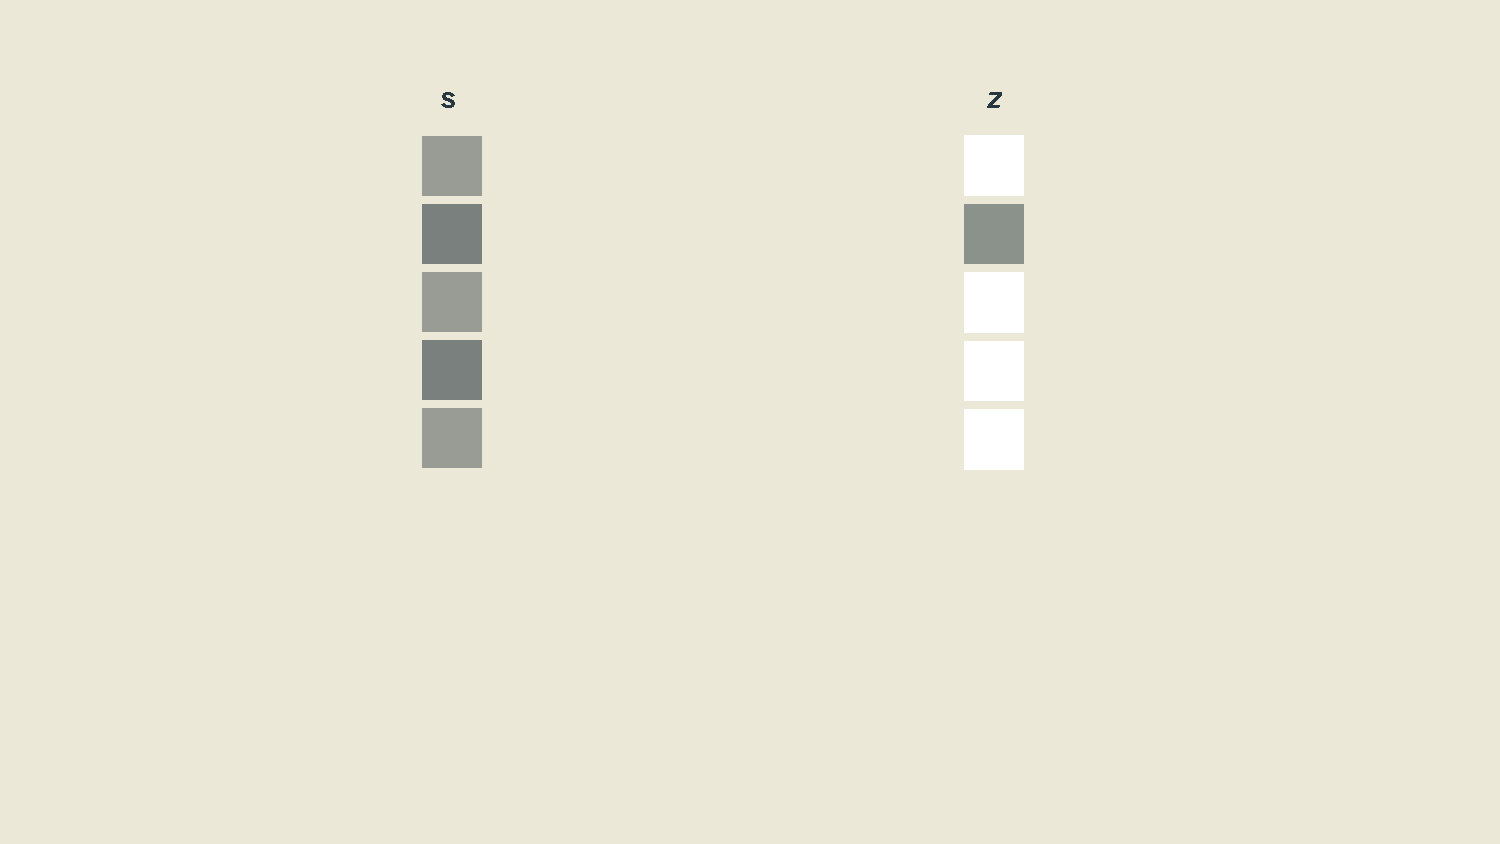
\includegraphics[width=\textwidth]{img/300_reparam_1.pdf}}
\only<4>{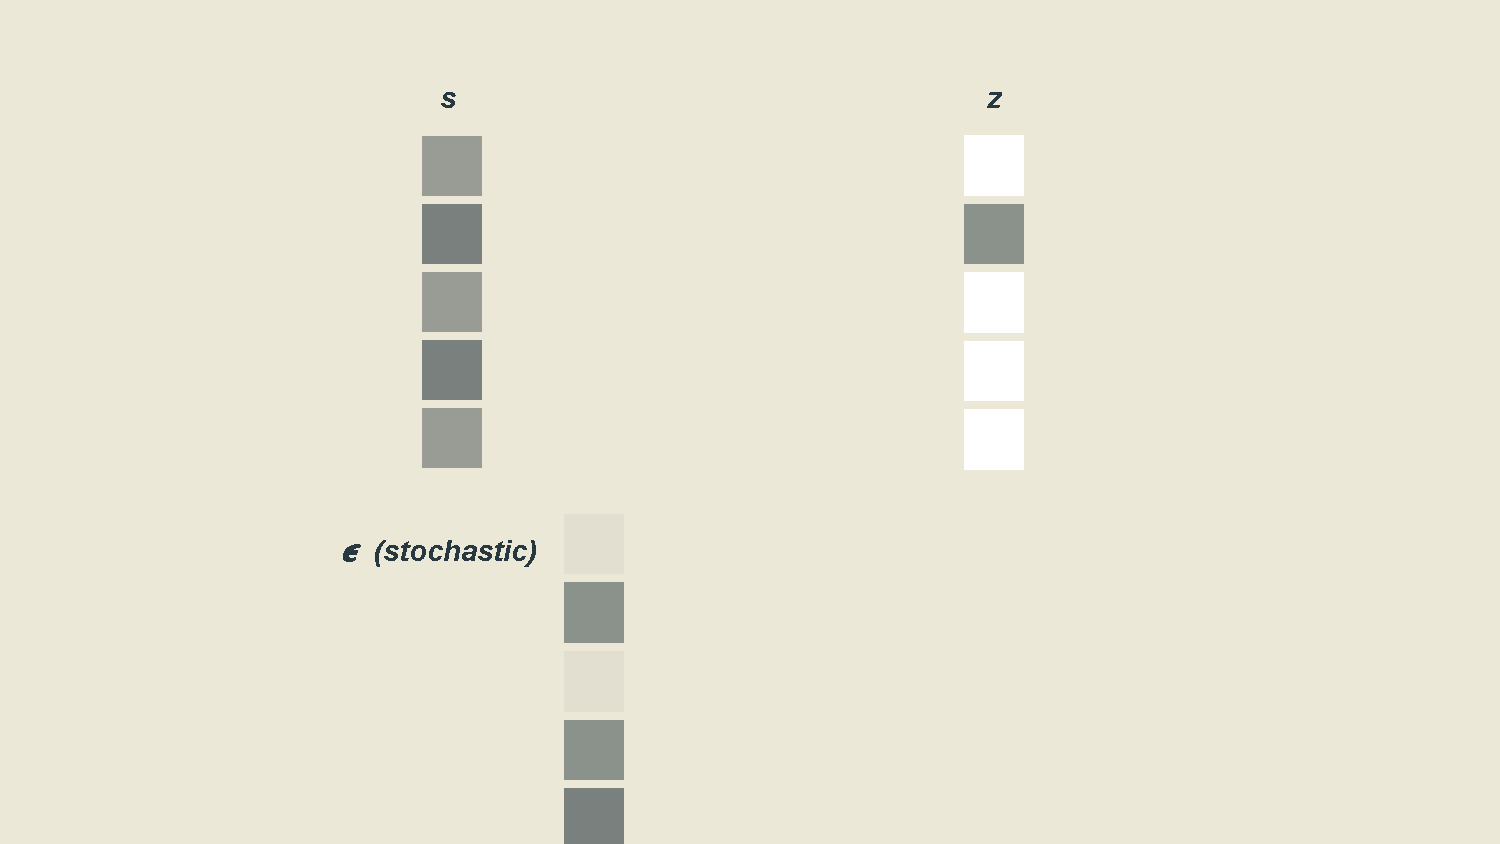
\includegraphics[width=\textwidth]{img/300_reparam_2.pdf}}
\only<5>{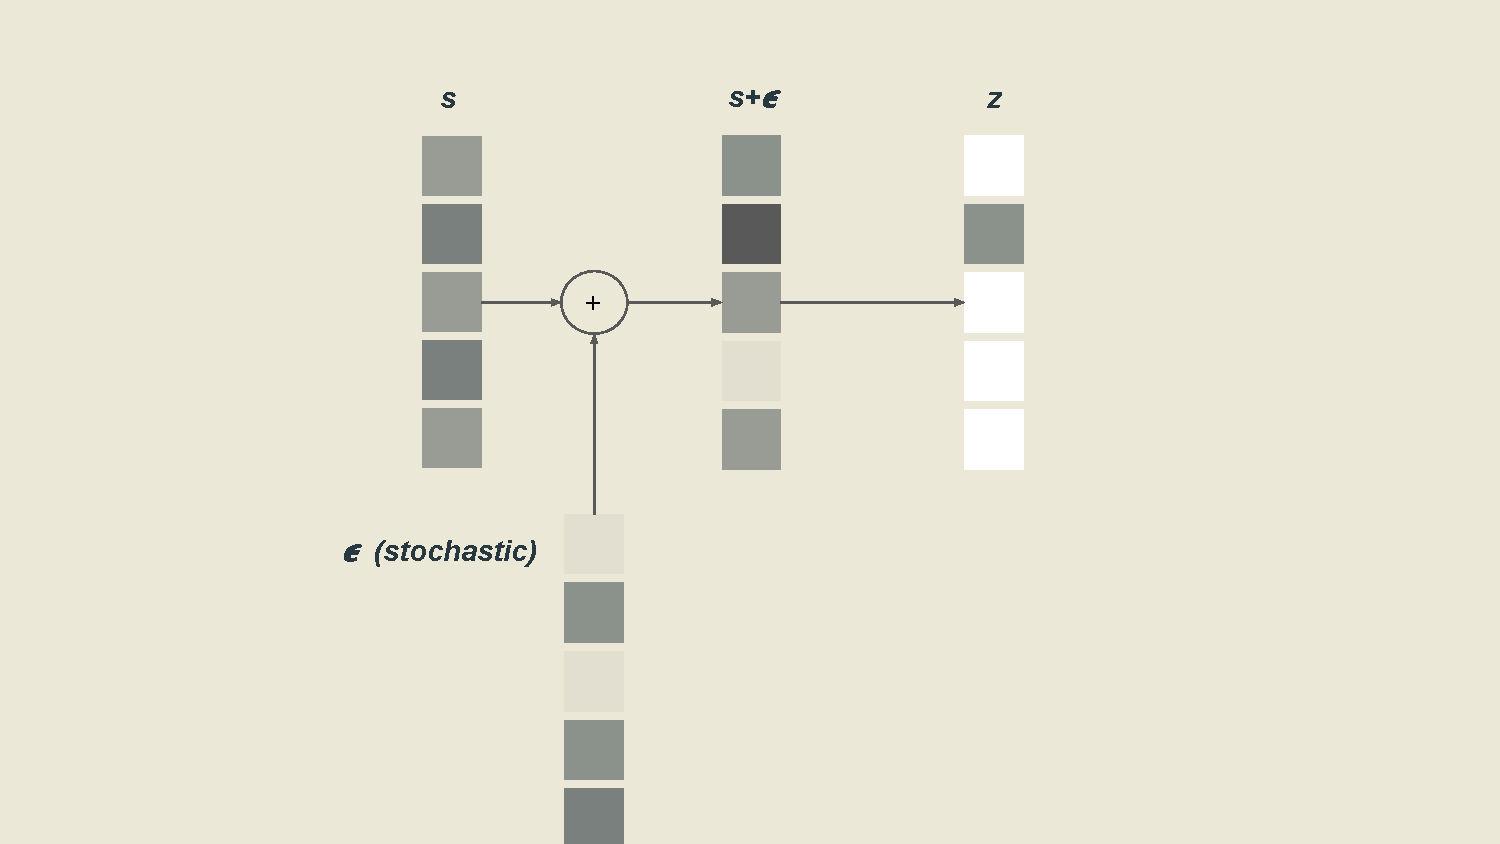
\includegraphics[width=\textwidth]{img/300_reparam_3.pdf}}
\only<6-7>{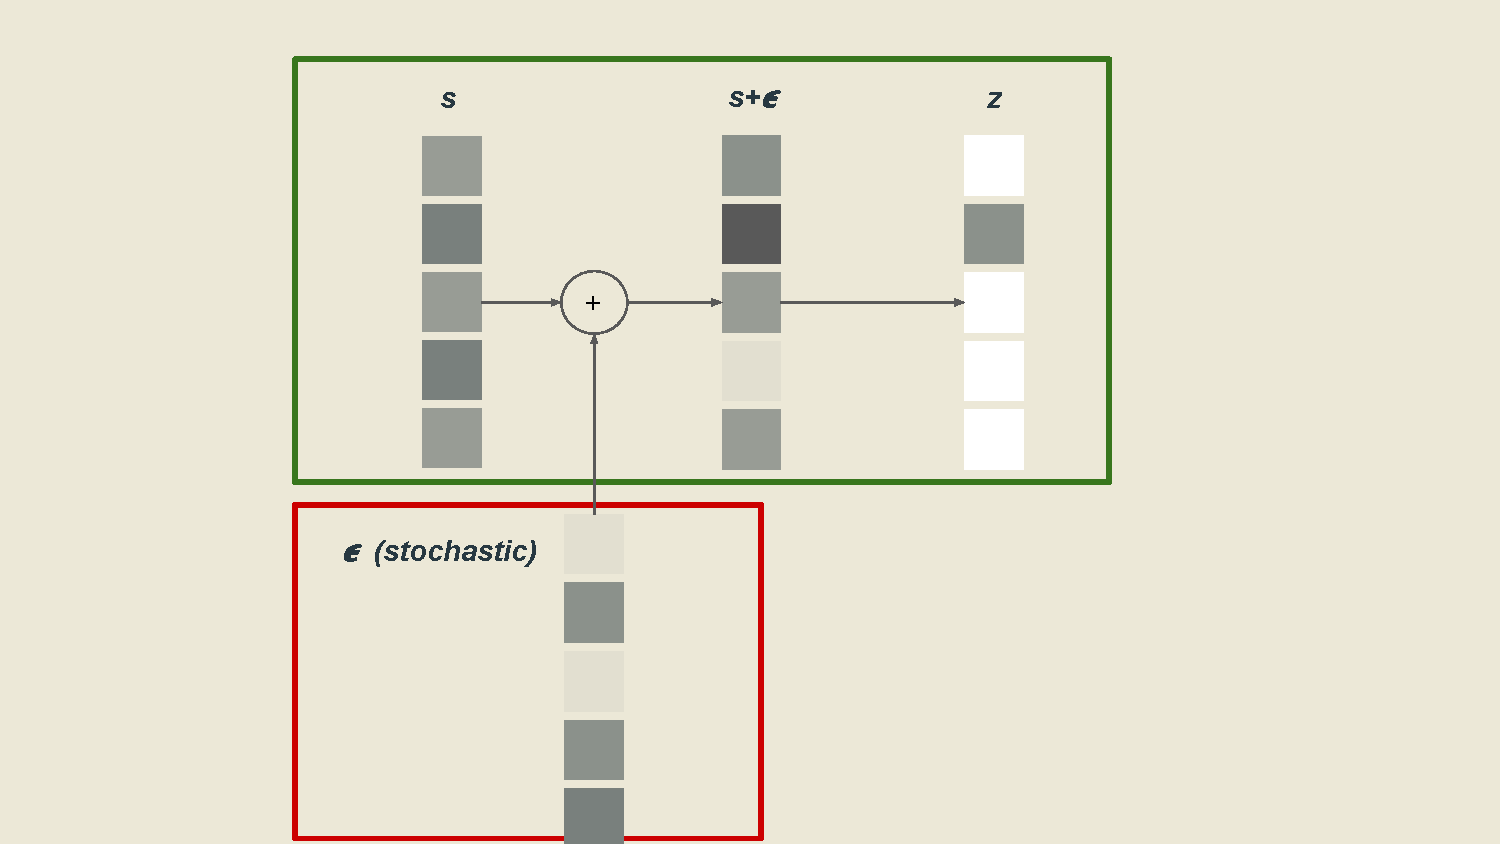
\includegraphics[width=\textwidth]{img/300_reparam_4.pdf}}
\end{column}
\end{columns}
\only<7>{\overlaybox{
\small
\underline{As a result:}\\
\small Stochasticity is moved as an input. \\
\small We can backpropagate through the deterministic input to $\z$.
}
}
\end{frame}


\begin{frame}%
\frametitle{Categorical reparameterization}%
\cornercite{jang2016categorical, maddison2016concrete}
\centering
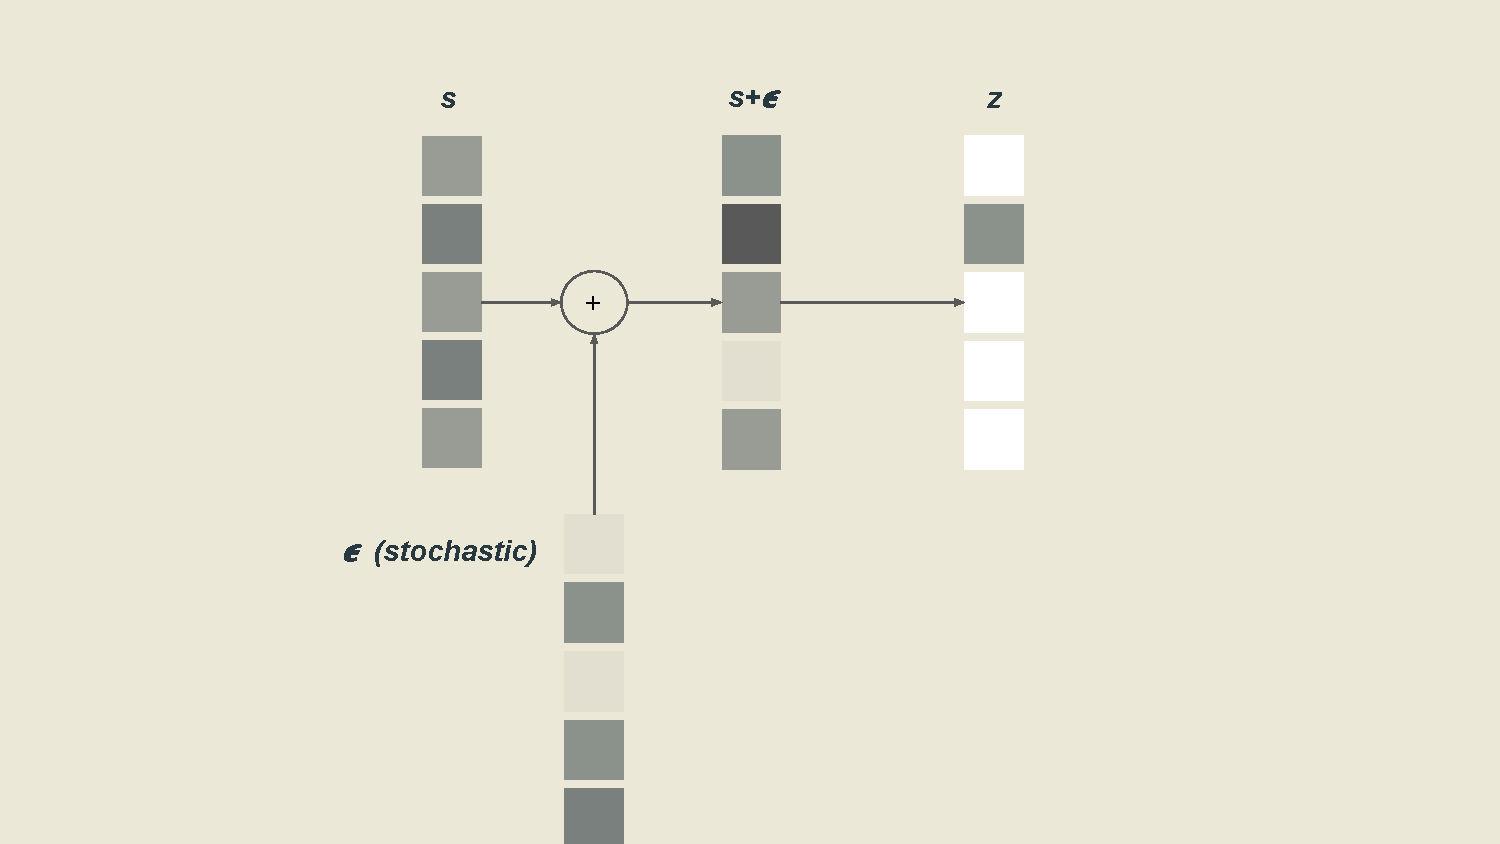
\includegraphics[width=0.8\textwidth]{img/300_reparam_3.pdf}%
\uncover<2->{\overlaybox{How do we sample from a categorical variable?}}
\end{frame}


\begin{frame}%
\frametitle{Sampling from a categorical variable}%
\framesubtitle{\small We want to sample from a categorical variable
    with scores $\s$ (class $i$ has a score $\ss_{i}$)}
\begin{columns}[t]%
\begin{column}{.5\textwidth}%
\centering%
\uncover<2->{\textbf{1. Inverse transform sampling:} \\}
\begin{itemize}
    \item<3-> $\p = \softmax(\s)$
    \item<4-> $c_{i} = \sum_{j \leq i} \pp_{j}$
    \item<5-> $u \sim \operatorname{Uniform}(0, 1)$
    \item<6-> return $\z = \bs{e}_t$ s.t.\ $c_{t} \leq u < c_{t+1}$
\end{itemize}
\end{column}
\begin{column}{.5\textwidth}%
\centering%
\uncover<7->{\textbf{2. The Gumbel-Max trick} \\}
\begin{itemize}
    \item<8-> $u_i \sim \operatorname{Uniform}(0, 1)$
    \item<9-> $\epsilon_{i} = -\log(-\log(u_i))$
    \item<10-> $\z = \argmax(\s + \bs{\epsilon})$
\end{itemize}
\end{column}
\end{columns}
\vspace{\baselineskip}
\centering
\uncover<11->{\small{The two methods are equivalent. \textit{(Not obvious, but we will not prove it now.)}}\\}
\uncover<12->{\small{Requires sampling from the Standard Gumbel Distribution G(0,1).}\\}
\uncover<13->{\small\textit{Derivation \& more info:
\citep{ryanadamsblog,timblog}}}
\uncover<14->{\overlaybox{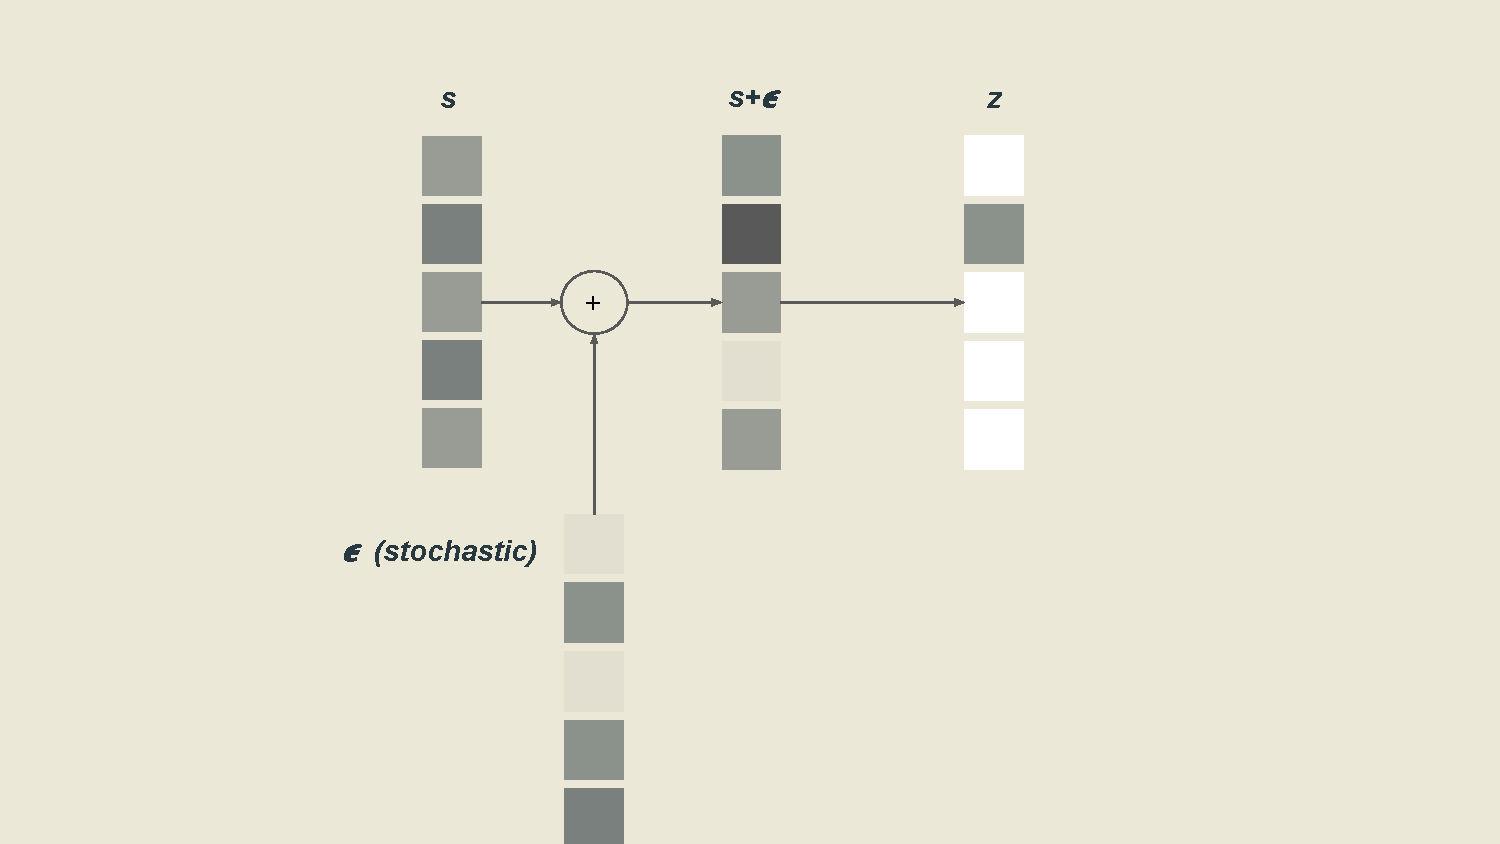
\includegraphics[width=.6\textwidth]{img/300_reparam_3.pdf}}}
\uncover<15->{\overlaybox{We have an argmax again\\
    and cannot backpropagate!}}
\end{frame}



\begin{frame}%
\frametitle{Straight-Through Gumbel Estimator}%
\framesubtitle{\small Apply a variant of the Straight-Through Estimator to Gumbel-Max!}
\cornercite{jang2016categorical, maddison2016concrete}
\centering
\begin{columns}[T]
\begin{column}{.4\textwidth}
% \small
\begin{itemize}
    \item<2->Forward: % $argmax$\\
    $\z = \argmax(\s + \bs{\epsilon})$
    \item<3->Backward: pretend we had done \\
    $\tilde\p = \softmax(\s + \bs{\epsilon})$
\end{itemize}
\end{column}
\begin{column}{.6\textwidth}
\only<2>{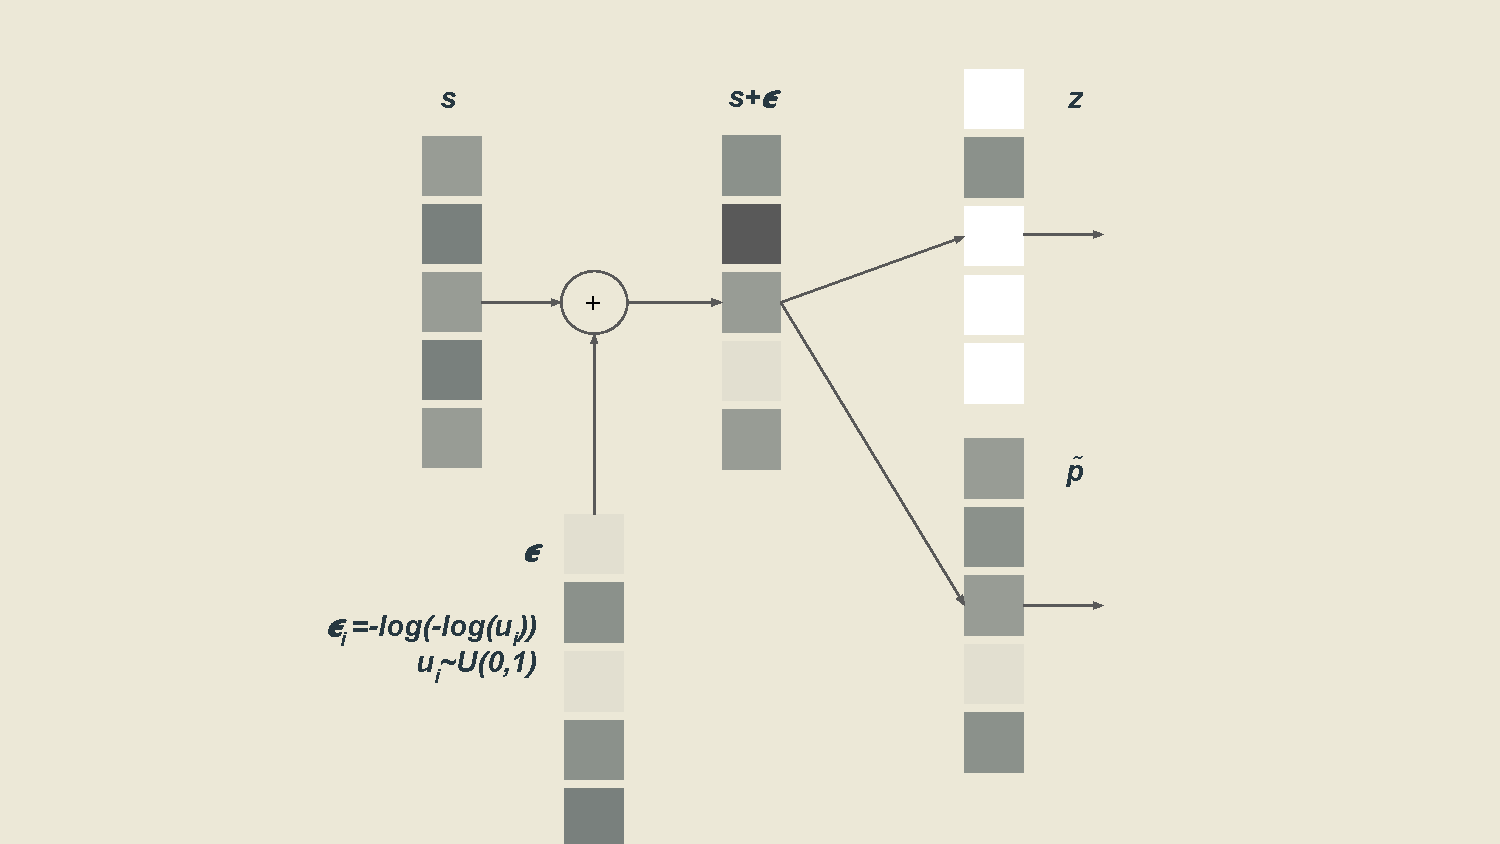
\includegraphics[width=\textwidth]{img/300_reparam_gumbel_st.pdf}}
\only<3-4>{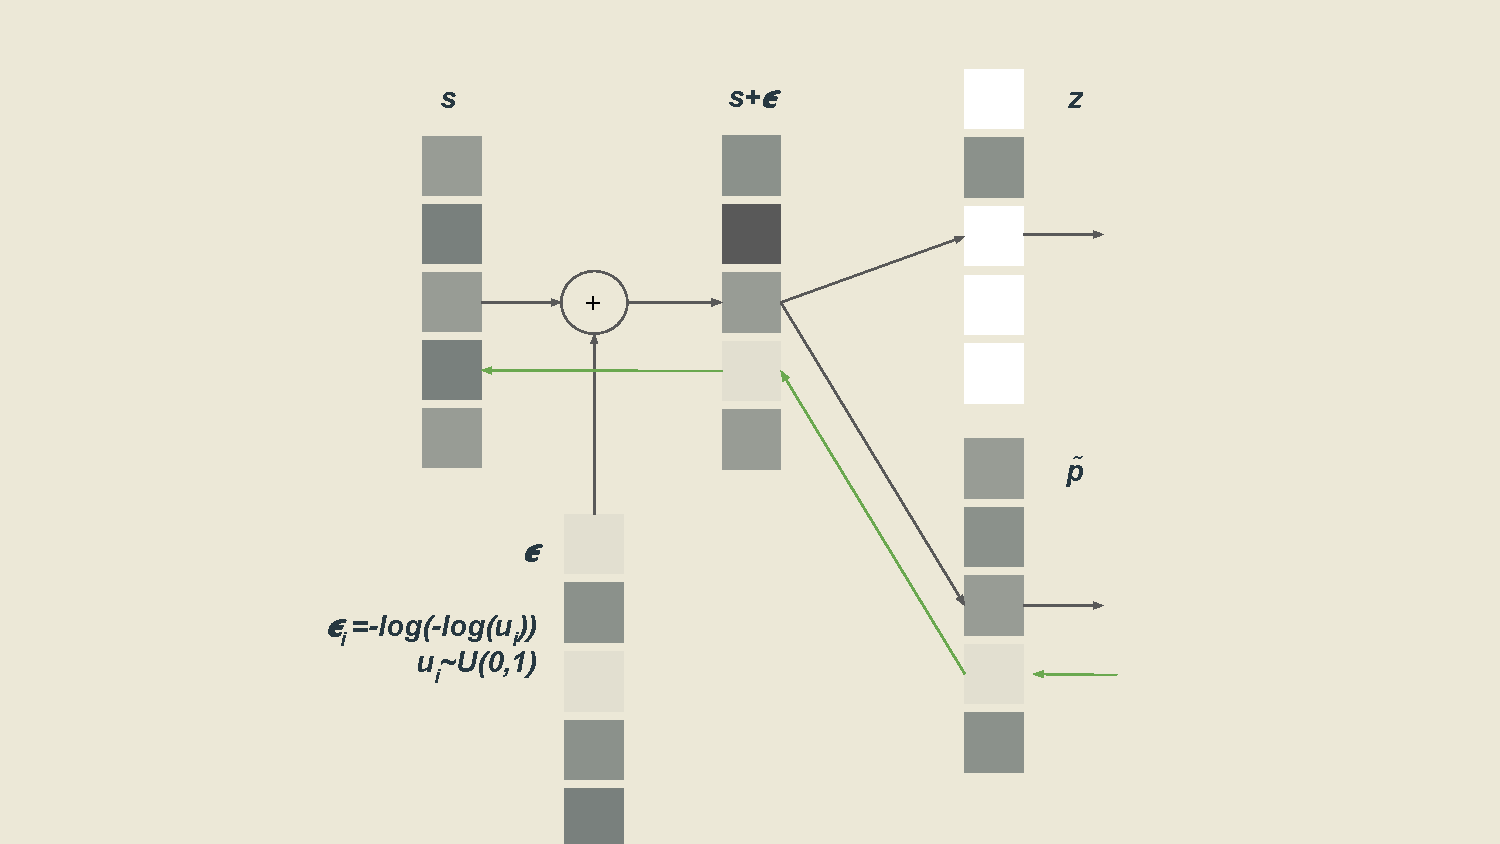
\includegraphics[width=\textwidth]{img/300_reparam_gumbel_st_back.pdf}}
\end{column}
\end{columns}
\uncover<4->{\overlaybox{What about the structured case?}}
\end{frame}


\againframe{structuretypes}


\begin{frame}%
\frametitle{Sampling from incremental structures}%
\centering
\begin{itemize}
    \item<2-> Build a structure as a sequence of discrete choices (e.g., shift-reduce)
    \item<3-> Assigns a score to any (partial structure, action) tuple.
    \item<4-> Reparameterize the scores with Gumbel-Max - now we have a deterministic node.
    \item<5-> \underline{Forward}: the \textbf{argmax} from the reparameterized scores for each step
    \item<6-> \underline{Backward}: pretend we had used a \textbf{differentiable surrogate function}
    \item[]<7-> \underline{Example}: Gumbel Tree-LSTM \citep{choi2017learning}.
\end{itemize}
\end{frame}


\begin{frame}%
\frametitle{Example: Gumbel Tree-LSTM}%
\cornercite{choi2017learning}
\centering
\small
\begin{itemize}
\item Building task-specific tree structures.
\item Straight-Through Gumbel-Softmax at each step to select one arc.
\end{itemize}
\begin{center}
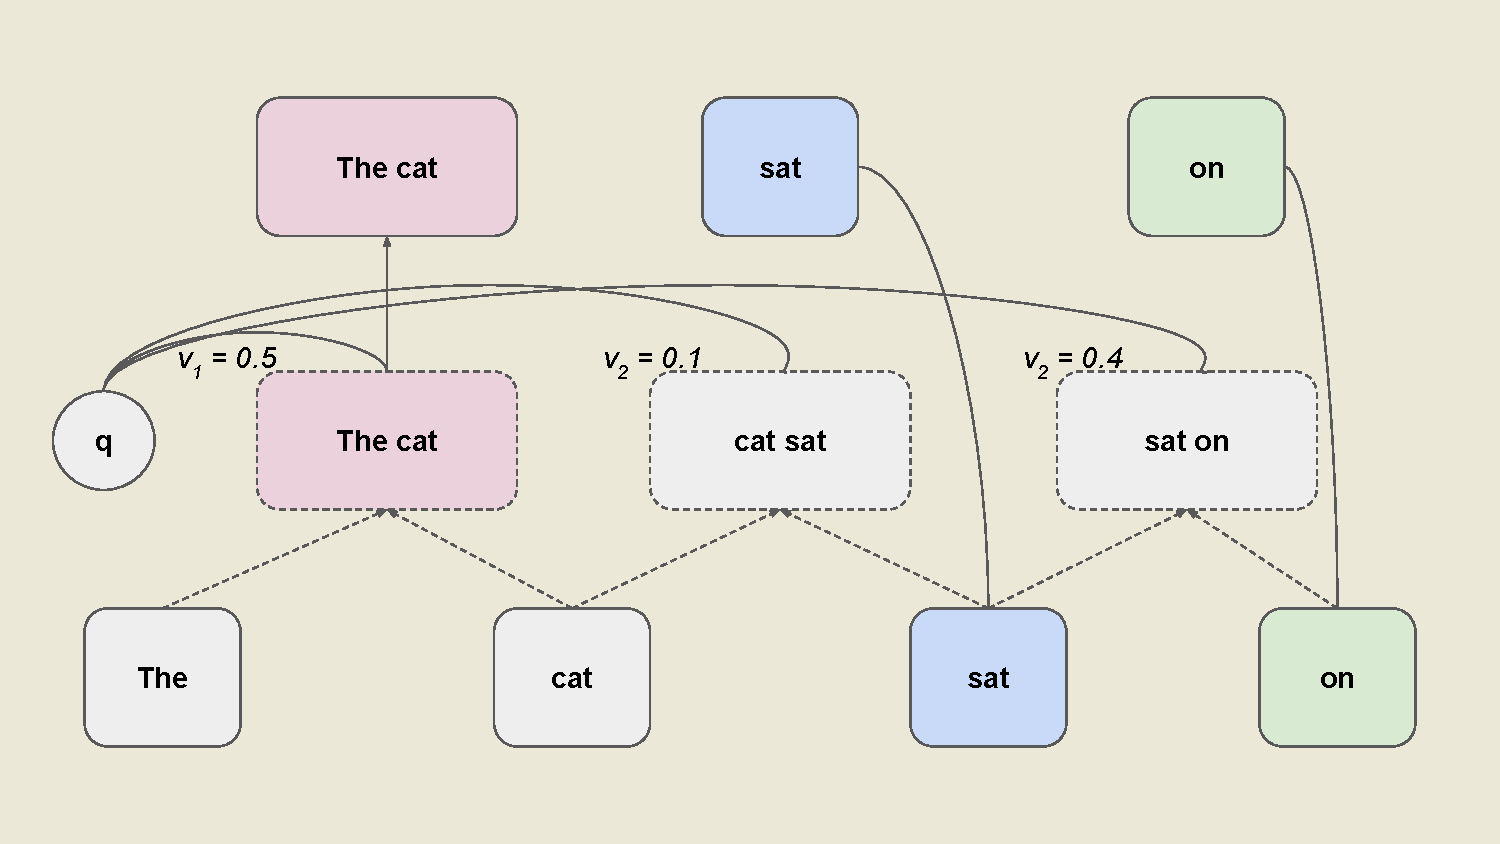
\includegraphics[width=0.6\textwidth]{img/300_gumbel_tree_lstm.pdf}%
\end{center}
\end{frame}



\begin{frame}%
\frametitle{Sampling from factorized models}%
\framesubtitle{Perturb-and-MAP}%
\cornercite{perturbandmap,corro2018differentiable,corro2019acl}
\centering
Reparameterize by \textbf{perturbing the arc scores}.
(inexact!)
\\[\baselineskip]
\begin{columns}[t]%
\begin{column}{.6\textwidth}%
\centering%
\begin{itemize}
    \item<2-> Sample from the normal Gumbel distribution.
    \item<3-> Perturb the arc scores with the Gumbel noise.
    \item<4-> Compute MAP (task-specific algorithm).
    \item<5-> Backward: we could use Straight-Through with Identity.
\end{itemize}
\end{column}
\begin{column}{.4\textwidth}%
\centering%
\begin{itemize}
    \item<2-> $\bs{\epsilon} \sim G(0,1)$
    \item<3-> $\tilde \pr = \pr + \bs{\epsilon}$
    \item<4-> $\argmax_{\z \in \ZZ} \tilde \pr ^\top \z$
\end{itemize}
\end{column}
\end{columns}
\end{frame}


\begin{frame}%
\frametitle{Summary: Gradient surrogates}%
\centering
\begin{itemize}
    \item Based on the \textbf{Straight-Through Estimator}.
    \item Can be used for stochastic or deterministic computation graphs.
    \item \textbf{Forward pass}: Get an argmax (might be structured).
    \item \textbf{Backpropagation}: use a function, which we hope is close to argmax.
    \item Examples:
        \begin{itemize}
            \item Argmax for iterative structures and factorization into parts
            \item Sampling from iterative structures and factorization into parts
        \end{itemize}
\end{itemize}
\end{frame}

% \begin{frame}%
% \frametitle{Examples: Gradient Surrogates}%
% \centering
% \begin{itemize}
%     \item Deterministic case.
%     \begin{itemize}
%         \item Identity on the backward pass. %\citep{corro2019acl}.
%         \item Marginals on the backward pass. %\citep{corro2019acl}.
%         \item SPIGOT (\citep{peng2018backpropagating})
%         \item Differentiable shift-reduce parsing (\citep{maillard2018latent}).
%     \end{itemize}
%     \item Examples for sampling latent structures.
%     \begin{itemize}
%         \item Perturb-and-MAP (\citep{corro2018differentiable}): Imitate sampling a tree by perturbing arc scores (an approximation of the real distribution.)
%         \item Gumbel Tree-LSTM (\citep{choi2017learning}):  Sample one action iteratively.
%     \end{itemize}
% \end{itemize}
% \begin{tabular}{l l{1in} l{1in}}
%     \small
%      & Deterministic & Stochastic \\
%     Iterative & Differentiable shift-reduce \citep{maillard2018latent} & Gumbel-TreeLSTM \citep{choi2017learning} \\
%     Factorized & SPIGOT \citep{peng2018backpropagating} & Perturb-and-Parse \citep{corro2018differentiable} \\
% \end{tabular}
% \end{frame}

\begin{frame}%
\frametitle{Gradient surrogates: Pros and cons}%
\centering
Pros
\begin{itemize}
    \item Do not suffer from the high variance problem of REINFORCE.
    \item Allow for flexibility to select or sample a latent structured in the middle of the computation graph.
    \item Efficient computation.
\end{itemize}
Cons
\begin{itemize}
    \item The Gumbel sampling with Perturb-and-MAP is an approximation.
    \item Bias, due to function mismatch on the backpropagation\\\quad(next section will address this problem.)
\end{itemize}
\end{frame}

\begin{frame}<1-2>[t,label=overview]%
\newcommand{\samp}{\textcolor{tPink}{\scriptsize SPL}}
\newcommand{\map}{\textcolor{tGreen}{\scriptsize MAP}}
\newcommand{\marg}{\textcolor{tBleu}{\scriptsize MRG}}
\setbeamertemplate{itemize/enumerate body begin}{\small}
\frametitle{Overview}%
\begin{columns}[T]%
\begin{column}{.333\textwidth}
\centering
$$\EE_{\parser}\big[L(\z)\big]$$
\begin{itemize}
\item REINFORCE\only<6->{\textsuperscript{\samp}}
\item Straight-Through Gumbel\\ \quad (Perturb \& MAP)%
\only<6->{\textsuperscript{\samp,\marg}}
\item<5-> SparseMAP\only<6->{\textsuperscript{\map{}+}}
\end{itemize}
\end{column}
\begin{column}{.333\textwidth}
\centering
$$L\big(\textstyle \argmax_z \parser\big)$$
\begin{itemize}
\item Straight-Through\only<6->{\textsuperscript{\map,\marg}}
\item SPIGOT\only<6->{\textsuperscript{\map{}+}}
\end{itemize}
\end{column}
\onslide<2->{%
\begin{column}{.333\textwidth}
\centering
$$L\big(\EE_{\parser}[\z]\big)$$
\begin{itemize}
\item<2,4-> Structured Attn. Nets\only<6->{\textsuperscript{\marg}}
\item<2,4-> SparseMAP\only<6->{\textsuperscript{\map{}+}}
\end{itemize}
\end{column}}
\end{columns}
%\only<4-5>{%
%\centering \small \textbf{Model restrictions:}\\
%\begin{columns}[T]%
%\begin{column}{.333\textwidth}
%\begin{itemize}
%\item  $\dom L$ may be only $\ZZ$,
%\item $\nabla_{\z} L$ need not exist!
%\end{itemize}
%\end{column}
%\begin{column}{.333\textwidth}
%\begin{itemize}
%\item $L(\z)$ with $\z \in \ZZ$ in forward
%\item needs (relaxed) $\nabla_{\z} L$ in backward.\\
%\end{itemize}
%\end{column}
%\begin{column}{.333\textwidth}
%\begin{itemize}
%\item $L(\z)$ must be relaxed\\ and differentiable.
%\item (sparsity gets us closer to $\ZZ$).
%\end{itemize}
%\end{column}
%\end{columns}
%}
\only<6->{%
\centering \small \textbf{Computation:}\\
\begin{itemize}
\item[] \samp{}: Sampling. (Simple in incremental/unstructured, hard for most
global structures.)
\item[] \map{}:  Finding the highest-scoring structure.
\item[] \marg{}:  Marginal inference.
\end{itemize}}
\onslide<2>{\overlaybox[.8]{And more, after the break!}}
\end{frame}

\section{End-to-end differentiable relaxations}
\sepframe{IV. End-to-end\\Differentiable Relaxations}
\begin{frame}[plain]%
\frametitle{End-to-end differentiable relaxations}
\begin{enumerate}
\item Digging into softmax
\item Alternatives to softmax
\item Generalizing to structured prediction
\item Stochasticity and global structures
\end{enumerate}
\end{frame}

\begin{frame}%
\frametitle{%
\alt<1>{Recall: Discrete choices \& differentiability}{One solution: smooth
relaxation}}
\centering
%
\def\vecwidth{.8}
\def\vecheight{.8}
\tikzset{elem/.style={ultra thick,mybg}}
%
\begin{tikzpicture}%
%
\node[anchor=south] at (-1-.5*\vecwidth, \vecheight*5+.1) {$\s$};

\drawcs
\drawscores
\onslide<1>{\drawargmax[\z]}
\onslide<2->{\drawsoftmax[\p]}

\draw[elem,fill=vecfg!50!vecbg] (-1-\vecwidth, \vecheight*4) rectangle (-1, \vecheight*5);
%\node[anchor=south] at (1+.5*\vecwidth, \vecheight*5+.1) {$\hat{\p}$};
\draw[elem,fill=vecbg]  (1, \vecheight*4) rectangle (1+\vecwidth, \vecheight*5);
\draw[elem,fill=vecfg!70!vecbg] (1, \vecheight*3) rectangle (1+\vecwidth, \vecheight*4);

\onslide<3>{\node at (1+.5*\vecwidth, \vecheight*2) {\emoji{frown}};}

\node[anchor=south,align=center] at (-6, \vecheight*3+1) (in) {\phantom{input}};
\node[anchor=south,align=center] at (6, \vecheight*3+1) (out) {\phantom{output}};
%
\node at (0, -1) {$\frac{\partial \alt<1>{\z}{\p}}{\partial \s}=$
\alt<1>{$\bs{0}$ {\small or n/a}}{\emoji{happ}}};
\node[anchor=south,align=center] at (-6, \vecheight*3+1) (in) {input\\$\bs{x}$};
\node[anchor=south] at (-2, \vecheight*3+1) (in-end) {};
\node[anchor=south,align=center] at (6, \vecheight*3+1) (out){output\\$\widehat{\bs{y}}$};
\node[anchor=south] at (2, \vecheight*3+1) (out-end) {};
%
\path (in) edge[->,very thick,bend right=50] node[anchor=north] (ff) {$\s =
    %\bs{f}_1(\bs{x};\bs{w})$} (in-end);
    \bs{f}_{\parp}(\bs{x})$} (in-end);
\path (out-end) edge[->,very thick,bend right=50] node[anchor=north] {$y =
    %f_2(\alt<1>{\z}{\p}, \bs{x}; \bs{w})$} (out);
    \bs{g}_{\clfp}(\z, \bs{x})$} (out);
\node at (0, -2) {\alt<1>{(argmax)}{(softmax)}};
\node<2->[font={\fontsize{10pt}{10}\selectfont},below=50pt of
ff,anchor=north,align=center] {%
$\p = \softmax(\s) = \EE[\z]$, i.e.\\
replace $\EE\big[f(\z)\big]$ with $f\big(\EE[\z]\big)$
};
\end{tikzpicture}
\\[6ex]
\begin{tikzpicture}[overlay]
    \draw[axisline,->] (3, 3) -- (3, 5.5) node[left] {$\pp_1$};
    \draw[axisline,->] (3, 3) -- (7, 3) node[right]{$\ss_1$};

    \node[axislabel,left] at (3, 3) {$0$};
    \node[axislabel,left] at (3, 5) {$1$};

    \draw[axisline] ($(3,3) + (-\ticksize, 0)$) -- ($(3,3) + (+\ticksize, 0)$);
    \draw[axisline] ($(3,4) + (-\ticksize, 0)$) -- ($(3,4) + (+\ticksize, 0)$);
    \draw[axisline] ($(3,5) + (-\ticksize, 0)$) -- ($(3,5) + (+\ticksize, 0)$);

    \draw[axisline] ($(3,3) + (0, -\ticksize)$) -- ($(3,3) + (0, +\ticksize)$);
    \draw[axisline] ($(4,3) + (0, -\ticksize)$) -- ($(4,3) + (0, +\ticksize)$);
    \draw[axisline] ($(5,3) + (0, -\ticksize)$) -- ($(5,3) + (0, +\ticksize)$);
    \draw[axisline] ($(6,3) + (0, -\ticksize)$) -- ($(6,3) + (0, +\ticksize)$);

    \node[axislabel,below] at (4, 3) {$\ss_2 - 1$};
    \node[axislabel,below] at (5, 3) {$\ss_2$};
    \node[axislabel,below] at (6, 3) {$\ss_2 + 1$};

    \draw[ultra thick,colorArgmax] (3, 3) -- (5,3) ;
    \draw[ultra thick,colorArgmax] (5, 5) -- (7,5) ;

\onslide<2->{%
    \draw (3, 3.1) edge[colorSoftmax,ultra thick,out=360,in=180,looseness=1.5] (7, 4.9);
}
\end{tikzpicture}%
\end{frame}

\againframe<3>{overview}

\begin{frame}[t,fragile]%
\frametitle{What is softmax?}%
\centering \fontsize{12pt}{15}\selectfont
Often defined via $\displaystyle
{\pp}_i = \frac{\exp \ss_i}{\sum_j \exp \ss_j}$,\quad
but where does it come from?% \\[1ex]
\begin{columns}
\begin{column}{.62\textwidth}
\centering
\begin{itemize}
\item<2->[] $\p \in \simplex$: probability distribution over choices
\item<6->[] Expected score under $\p$: $\EE_{i \sim \p}~\ss_i =\p^\top\s$
\item<7->[] \textbf{argmax} \onslide<8->{maximizes \textbf{expected score}}
\item<9->[] Shannon entropy of $\p$: $\HH(\p) = -\sum_i \pp_i \log \pp_i$
\item<10->[] \textbf{softmax} maximizes \textbf{expected score} $+$ \textbf{entropy}:
\end{itemize}
\end{column}%
\begin{column}{.33\textwidth}
\begin{overlayarea}{\textwidth}{6\baselineskip}
\centering
\only<9>{%
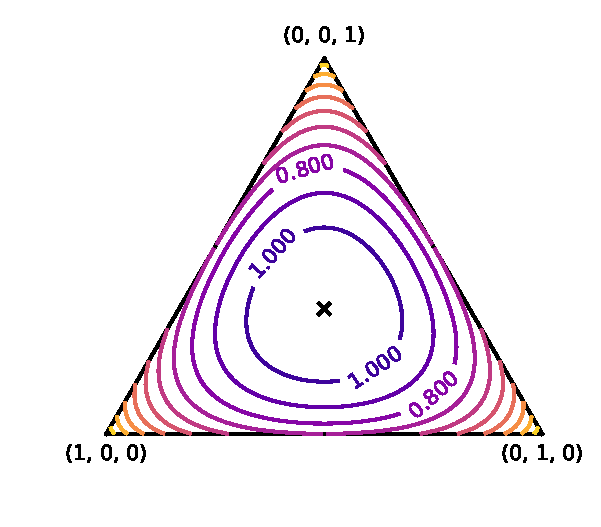
\includegraphics[width=.99\textwidth]{img/4011_simplex_0_softmax.pdf}
}%
\only<10>{%
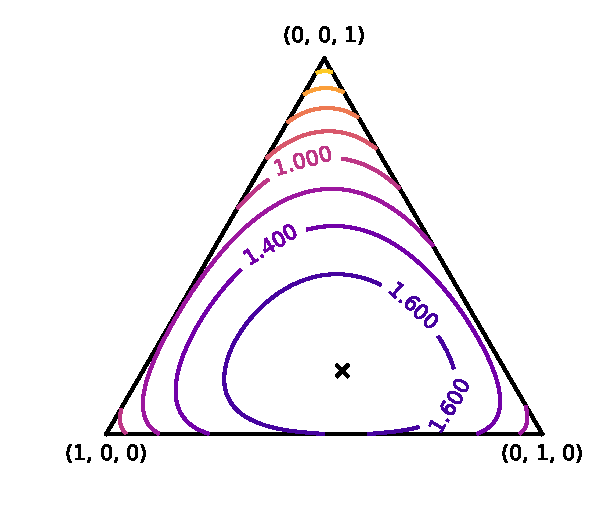
\includegraphics[width=.99\textwidth]{img/4011_simplex_1_softmax.pdf}\\
$\displaystyle \argmax_{\p \in \simplex} \p^\top\s + \HH(\p)$
}%
\onslide<2-8>{%
\begin{tikzpicture}[every node/.style={inner sep=0,outer sep=2pt}]
    \begin{axis}[
        small,
        xmin=-.1, xmax=1.5,
        ymin=-.1, ymax=1.5,
        zmin=-.1, zmax=1.5,
        height=6cm,
        width=8cm,
        xtick={0, .5, 1, 1.5},
        ytick={.5, 1, 1.5},
        ztick={.5, 1, 1.5},
        axis line style=thick,
        axis lines=middle,
        axis equal,
        compat=1.6,
        view={60}{15}
        ]

    \node at (axis cs:1, 0, 0) (A) {};
    \node at (axis cs:0, 1, 0) (B) {};
    \node at (axis cs:0, 0, 1) (C) {};

    \only<2->{%
    \addplot3[color=tDY,ultra thick,fill=tDY,fill opacity=.5] coordinates { (0,0,1) (0,1,0) (1,0,0) (0,0,1) };

    \draw[tBleu,fill] (A) circle[radius=2pt];
    \draw[tBleu,fill] (B) circle[radius=2pt];
    \draw[tBleu,fill] (C) circle[radius=2pt];
    }

    \def\ofst{.3,.3,.4}
    \only<3>{%
    \node[anchor=south west,font=\small]
        at ($(B) + .5*(axis direction cs:\ofst)$)
        (lblB) {$\p = [0, 1, 0]$};
    \draw[thick,fg,->] (lblB.south west) -- (B);
    }

    \only<4>{%
    \node[anchor=south west,font=\small]
        at ($(C) + (axis direction cs:\ofst)$)
        (lblC) {$\p = [0, 0, 1]$};
    \draw[thick,fg,->] (lblC.south west) -- (C);
    }

    \only<5>{%
    \node at (axis cs:.33,.33,.33) (mid) {};
    \draw[tBleu,fill] (mid) circle[radius=2pt];
    \node[anchor=south west,font=\small]
        at ($(mid) + (axis direction cs:\ofst)$)
        (lblmid) {$\p = \left[\nicefrac{1}{3}, \nicefrac{1}{3},
    \nicefrac{1}{3}\right]$};
    \draw[thick,fg,->] (lblmid.south west) -- (mid);
    }

    \only<6->{%
        \node[anchor=west,label=east:{\small $\s=[.7, .1, 1.5]$}] at
        (axis cs:.7,.1,1.5) (s) {};
        \draw[tVividBlue,fill] (s) circle[radius=2pt];
    }
    \only<6->{%
        % We cannot use foreach inside pgfplots axis environment.
        % also, we need fragile AND double the ##
        \pgfplotsinvokeforeach{90,80,...,10}{
            \draw[ultra thick,tPeony!##1!tTarmac]
            %(axis cs: .05+1-.01*##1,0,-.05+.01*##1)  % slignt .05 skew
            (axis cs: 1-.01*##1,0,.01*##1)  % slignt .05 skew
            -- (axis cs: 0,1-.01*##1,.01*##1);
        }
    }
    \only<8->{
        \node[anchor=south west,font=\small]
            at ($(C) + (axis direction cs:.3,.3,-.1)$)
            (lblCstar) {$\p^\star = [0, 0, 1]$};
        \draw[thick,fg,->] (lblCstar.west) -- (C);
        \draw[colorArgmax,fill] (C) circle[radius=3pt];
    }

    \end{axis}
\end{tikzpicture}}%
\\
\only<8->{%
$\displaystyle \argmax_{\p \in \simplex} \p^\top\s$
\\[1ex]
}
\end{overlayarea}
\end{column}
\end{columns}
\end{frame}

\begin{frame}[t]
\frametitle{Variational form of softmax}
\small
\setlength{\abovedisplayskip}{5pt}%
\setlength{\belowdisplayskip}{5pt}%
\setlength{\abovedisplayshortskip}{0pt}%
\setlength{\belowdisplayshortskip}{0pt}
\centering
\textbf{Proposition.} The unique solution to~~
$\displaystyle \argmax_{\p \in \simplex} \p^\top\s + \HH(\p)$
~~is given by $\pp_j = \frac{\exp \ss_j}{\sum_i \exp \ss_i}$.
\\[\baselineskip]
\begin{columns}[t]
\begin{column}{.49\textwidth}
\uncover<2->{%
Explicit form of the optimization problem:
\begin{align*}
\text{maximize}\quad&\textstyle \sum_j \pp_j \ss_j - \pp_j \log \pp_j \\
\text{subject to}\quad& \p \geq 0,~\p^\top \bs{1} = 1
\end{align*}}
\uncover<3->{%
Lagrangian:
$$\mathcal{L}(\p, \bs{\nu}, \tau) = \textstyle -\sum_j \pp_j \ss_j - \pp_j \log \pp_j - \p^\top\bs{\nu} + \tau(\p^\top\bs{1} - 1)$$}
\uncover<4->{%
Optimality conditions (KKT):
\begin{align*}
0 &= \nabla_{p_i} \mathcal{L}(\p, \bs{\nu}, \tau) = -\ss_i + \log \pp_i + 1 - \nu_i +
\tau
\\
\p^\top\bs{\nu} &= 0 \\
\p &\in \triangle \\
\bs{\nu} &\geq \bs{0} \\
\end{align*}}
\end{column}
\begin{column}{.45\textwidth}
\uncover<5->{$\log \pp_i = \ss_i + \nu_i - (\tau + 1)$}\\
\uncover<6->{\quad if $\pp_i = 0$, r.h.s.\ must be $-\infty$,\\
\quad thus $\pp_i > 0$, so $\nu_i = 0$.\\[1ex]}
\uncover<7->{$\pp_i = \nicefrac{\exp(\ss_i)}{\exp(\tau + 1)} =
\nicefrac{\exp(\ss_i)}{Z}$\\[1ex]}
\uncover<8->{Must find $Z$ such that $\sum_j \pp_j = 1$. \\}
\uncover<9->{Answer:  $Z = \sum_j \exp(\ss_j)$ \\[1ex]}
\uncover<10->{So, $\displaystyle \pp_i = \frac{\exp(\ss_i)}{\sum_j \exp(\ss_j)}$. \\[3ex]
\textcolor{mygr}{Classic result, e.g., \citep{boyd,Wainwright2008}}}
\end{column}
\end{columns}
\end{frame}


\begin{frame}[t]
\frametitle{Generalizing softmax: Smoothed argmaxes}
\vspace{-.5\baselineskip}
\begin{columns}[T]
\begin{column}{.58\textwidth}
\centering
$\displaystyle \mapo(\s) = \argmax_{\p \in \simplex} \p^\top\s - \Omega(\p)$
\fontsize{12.5pt}{13}\selectfont%
\\
%{
\def\vph{\vphantom{$\sum_j$}}
\renewcommand{\arraystretch}{1.7}
\begin{tabular}{r@{~}r@{:~~}r@{$\,=\,$}l}
\onslide<3->{
\colorbul{colorArgmax} &
argmax    & $\Omega(\p)$ & \vph $0$ \\}
\onslide<4->{
\colorbul{colorSoftmax} &
softmax   & $\Omega(\p)$ & $\sum_j \pp_j \log \pp_j$ \\}
\onslide<5->{
\colorbul{colorSparsemax} &
sparsemax & $\Omega(\p)$ & \vph $\nicefrac{1}{2} \|\p\|^2_2$ \\}
\onslide<6->{
%\multicolumn{4}{l}{\footnotesize Generalized entropy in between:}\\
&$\alpha$-entmax  & $\Omega(\p)$ & \vph
    $\nicefrac{1}{\alpha(\alpha-1)} \sum_j \pp_i^\alpha$\\%
}
\only<7->{
%\colorbul{colorFusedmax} &
&
fusedmax  & $\Omega(\p)$ & \vph
    $\nicefrac{1}{2} \|\p\|^2_2 + \sum_j |\pp_j -\pp_{j-1}|$\\%
%\colorbul{colorFusedmax} &
&
csparsemax  & $\Omega(\p)$ & \vph
    $\nicefrac{1}{2} \|\p\|^2_2 + \iota(\bs{a} \leq \p \leq \bs{b})$\\%
&
csoftmax  & $\Omega(\p)$ & \vph
$\sum_j \pp_j \log \pp_j + \iota(\bs{a} \leq \p \leq \bs{b})$\\%
}
\end{tabular}%

\small
\only<6>{Generalized entropy interpolates in between \citep{Tsallis1988}\\
Used in Sparse Seq2Seq: \citep{sparseseq} \\ (Mon 13:50, poster session 2D)}
% Monday, 13:50, poster session 2D
%}%
\end{column}%
%
%
\begin{column}{.30\textwidth}
\centering
% BEGIN softmax 2d plot
\begin{tikzpicture}[baseline=(current bounding box.north),scale=.9]
    \draw[axisline,->] (3, 3) -- (3, 5.5) node[left] {$\pp_1$};
    \draw[axisline,->] (3, 3) -- (7, 3) node[right]{$\ss_1$};

    \node[axislabel,left] at (3, 3) {$0$};
    \node[axislabel,left] at (3, 5) {$1$};

    \draw[axisline] ($(3,3) + (-\ticksize, 0)$) -- ($(3,3) + (+\ticksize, 0)$);
    \draw[axisline] ($(3,4) + (-\ticksize, 0)$) -- ($(3,4) + (+\ticksize, 0)$);
    \draw[axisline] ($(3,5) + (-\ticksize, 0)$) -- ($(3,5) + (+\ticksize, 0)$);

    \draw[axisline] ($(3,3) + (0, -\ticksize)$) -- ($(3,3) + (0, +\ticksize)$);
    \draw[axisline] ($(4,3) + (0, -\ticksize)$) -- ($(4,3) + (0, +\ticksize)$);
    \draw[axisline] ($(5,3) + (0, -\ticksize)$) -- ($(5,3) + (0, +\ticksize)$);
    \draw[axisline] ($(6,3) + (0, -\ticksize)$) -- ($(6,3) + (0, +\ticksize)$);

    \node[axislabel,below] at (4, 3) {$-1$};
    \node[axislabel,below] at (5, 3) {$0$};
    \node[axislabel,below] at (6, 3) {$1$};

    \draw<3->[ultra thick,colorArgmax] (3, 3) -- (5,3) ;
    \draw<3->[ultra thick,colorArgmax] (5, 5) -- (7,5) ;
    \draw<4-> (3, 3.1)
        edge[colorSoftmax,ultra thick,out=360,in=180,looseness=1.5] (7, 4.9);
    \draw<5->[ultra thick,colorSparsemax,dashed]
        (3, 3) -- (4,3) -- (6,5) -- (7, 5) ;
\end{tikzpicture}%
% END softmax 2d plot
%\vspace{-.5cm}%
\\
% BEGIN Simplex barycentric
\begin{tikzpicture}[baseline=(current bounding box.north)]
\setupsimplexbary{}
\coordinate (argmax)    at (barycentric cs:L1=0,L2=0,L3=1);
\coordinate (softmax)   at (barycentric cs:L1=.3,L2=.2,L3=.5);
\coordinate (sparsemax) at (barycentric cs:L1=.3,L2=0,L3=.7);

\uncover<3->{%
\node[label=west:{\small $[0,0,1]$}] at (argmax) {};
\draw[point,fill=colorArgmax] (argmax) circle[radius=5pt];}
\uncover<4->{%
\node[label=south:{\small $[.3,.2,.5]$}] at (softmax) {};
\draw[point,fill=colorSoftmax] (softmax) circle[radius=5pt];}
\uncover<5->{%
\node[label=west:{\small $[.3,0,.7]$}] at (sparsemax) {};
\draw[point,fill=colorSparsemax] (sparsemax) circle[radius=5pt];}
\end{tikzpicture}%
%% END Simplex Barycentric
\end{column}%
\end{columns}%
%
\onslide<1-4>{\cornercite{sparseattn}}
\onslide<5>{\cornercite{sparseattn,sparsemax}}
\onslide<6>{\cornercite{sparseattn,fylosses}}
\onslide<7>{\cornercite{sparseattn,easy,Malaviya2018ACL}}
%\begin{tikzpicture}[font=\footnotesize,remember picture,overlay]
    %\node<6>[anchor=north east] at (current page.north east) {
        %\citep{sparseattn}};
    %\node<5>[anchor=south west] at (current page.south west) {
        %\citep{sparsemax}};
%\end{tikzpicture}
%\onslide<2>{\overlaybox{$\bs{\pi}_{\Omega}$ differentiable when $\Omega$
%strongly convex.}}
\end{frame}%

\againframe<4>{marginalpoly}

% MAIN IDEA
%
\begin{frame}<1-7>[label=mainidea]%
\onslide<8->{\cornercite{sparsemap}}%
\vspace{-\baselineskip}
\begin{columns}[T]%
\begin{column}{.45\textwidth}\centering%
\vbox to .9\textheight{%
{%
\fontsize{12.5pt}{13}\selectfont%
\setlength{\tabcolsep}{2pt}%
\renewcommand{\arraystretch}{2}%
\begin{tabular}{r r l}
\onslide<2->{%
\colorbul{colorArgmax} &
\textbf{argmax} &
$\displaystyle \argmax_{\p \in \triangle} \p ^\top \s$ \\
}
\onslide<4->{%
\colorbul{colorSoftmax} &
\textbf{softmax} &
$\displaystyle \argmax_{\p \in \triangle} \p ^\top \s + \HH(\p)$ \\
}
\onslide<8->{%
\colorbul{colorSparsemax} &
\textbf{sparsemax} &
$\displaystyle \argmax_{\p \in \triangle} \p ^\top \s - \nicefrac{1}{2} \|\p\|^2$
}%
\end{tabular}%
}
\vfill
\begin{tikzpicture}
\setupsimplexbary[2.5]{}
\coordinate (argmax)    at (barycentric cs:L1=0,L2=0,L3=1);
\coordinate (softmax)   at (barycentric cs:L1=.3,L2=.2,L3=.5);
\coordinate (sparsemax) at (barycentric cs:L1=.3,L2=0,L3=.7);

\onslide<2->{
\draw[point,fill=colorArgmax] (argmax) circle[radius=5pt];
}
\onslide<4->{
\draw[point,fill=colorSoftmax] (softmax) circle[radius=5pt];
}
\onslide<8->{
\draw[point,fill=colorSparsemax] (sparsemax) circle[radius=5pt];
}
\end{tikzpicture}}\end{column}
\begin{column}{.54\textwidth}\centering
\vbox to .9\textheight{%
{%
\fontsize{12.5pt}{13}\selectfont%
\setlength{\tabcolsep}{2pt}%
\renewcommand{\arraystretch}{2}%
\begin{tabular}{r l l@{\quad}}
\onslide<3->{%
\textbf{MAP} &
$\displaystyle \argmax_{\mg \in \Mp} \mg ^\top \pr$ &
\colorbul{colorArgmax} \\
}%
\onslide<5->{%
\textbf{marginals} &
$\displaystyle \argmax_{\mg \in \Mp} \mg ^\top \pr + \widetilde{\HH}(\mg)$ &
\colorbul{colorSoftmax} \\
}%
\onslide<9->{%
\textbf{SparseMAP} &
$\displaystyle \argmax_{\mg \in \Mp} \mg ^\top \pr - \nicefrac{1}{2} \|\mg\|^2$ &
\colorbul{colorSparsemax}
}%
\end{tabular}%
}
\vfill
\begin{tikzpicture}[node distance=0pt]%
\uncover<1->{
\node[
    ultra thick,
    draw=colorPolytope,
    fill=colorPolytope,
    fill opacity=.15,
    minimum size=2.5cm,
    regular polygon, regular polygon sides=6] (mp) {};
\node[label=east:{\small$\mathcal{M}$}] at (mp.corner 5) {};
\foreach \i in {1, ..., 6}%
{
    \draw[colorPolytope,fill] (mp.corner \i) circle[radius=3pt];
}
}
\coordinate (L1) at (mp.corner 3);
\coordinate (L2) at (mp.corner 5);
\coordinate (L3) at (mp.corner 2);
\coordinate (argmax)    at (L3);
\coordinate (softmax)   at (barycentric cs:L1=.25,L2=.25,L3=.45);
\coordinate (sparsemax) at (barycentric cs:L1=.4,L3=.6);
\onslide<3->{
    \draw[point,fill=colorArgmax] (argmax) circle[radius=5pt];
    \node[above right=of argmax] {\cartoon[.5]{1/4,2/5}};
}
\onslide<5->{
    \draw[point,fill=colorSoftmax] (softmax) circle[radius=5pt];
    \node[below right=of softmax] {\cartoonDense[.5]{}};
}
\onslide<9->{
    \draw[point,fill=colorSparsemax] (sparsemax) circle[radius=5pt];
    \node[left=of sparsemax] {\cartoonSparse[.5]{}};
}
\end{tikzpicture}}\end{column}
\end{columns}
%
%\begin{tikzpicture}[font=\footnotesize,remember picture,overlay]
    %\node<14>[anchor=north east] at (current page.north east) {
        %\textcolor{mygr}{\citep{sparsemap}}};
%\end{tikzpicture}
%\uncover<2-4>{\overlaybox[.33]{
%$\begin{aligned}
    %\Mp &\defeq \conv \big\{ \bs{a}_y : y \in \mathcal{Y} \big\} \\
    %\uncover<3-4>{&= \big\{ \bs{A}\p : \p \in \triangle \big\}} \\
    %\uncover<4>{&= \big\{ \EE_{Y\sim\p}~\bs{a}_Y : \p \in \triangle \big\}}
%\end{aligned}$
%}}
\uncover<6-7>{\overlaybox[.5]{%
    Just like softmax relaxes argmax,\\ marginals relax MAP
\textbf{differentiably}!}}
\uncover<7-7>{\overlaybox[.7]{%
Unlike argmax/softmax, computation is not obvious!}}
\end{frame}

\againframe<2->{algos}

\begin{frame}[t]
\frametitle{Derivatives of marginals 1: DP}
\centering
\begin{itemize}
\item[]<1-> \textbf{Dynamic programming:} marginals by \textbf{Forward-Backward},
\textbf{Inside-Outside}, etc.
\begin{itemize}
\item<3->
Alg. consists of differentiable ops:
PyTorch autograd can handle it! (v. bad idea)
\item<4-> Better book-keeping: \citet{Li2009}, \citet{arthurdp}
\item<5-> With circular dependencies, this breaks! Can get an approximation \citet{ves}
\end{itemize}
\end{itemize}
\vspace{-.5\baselineskip}
\uncover<2->{%
\begin{minipage}{.55\textwidth}
\begin{algorithm}[H]
\caption*{Marginals in a sequence tagging model.}
\setstretch{1.3}
\fontsize{9pt}{9}\selectfont
\begin{algorithmic}[1]
\State input:  $d$ tags, $n$ tokens,
                $\pr_U \in \reals^{n \times d},
                 \pr_V \in \reals^{d \times d}$
\State initialize $\bs{\alpha}_1 = \bs{0}, \bs{\beta}_n = \bs{0}$
\For{$i \in 2, \dots, n$}
\Comment{forward log-probabilities}
%\State $\alpha_{i,k} = (\pr_U)_{i,k} + \log \sum_{k'} \exp
%\big(
%\alpha_{i-1, k'} + (\pr_V)_{k', k}
%\big)
    \State $\alpha_{i,k} = \log \sum_{k'} \exp
\big(
\alpha_{i-1, k'} +
(\pr_U)_{i, k} +
(\pr_V)_{k', k}
\big)$
\hfill for all $k$
\EndFor

\For{$i \in n-1, \dots, 1$}
\Comment{backward log-probabilities}
\State $\beta_{i,k} = \log \sum_{k'} \exp
\big(
\beta_{i+1, k'} + (\pr_U)_{i+1, k'} + (\pr_V)_{k, k'}
\big)$
\hfill for all $k$
\EndFor
\State $Z = \sum_k \exp  \alpha_{n,k}$
\Comment{partition function}
\State \Return $\mg = \exp \big(\bs{\alpha} + \bs{\beta} - \log Z\big)$
\Comment{marginals}
\end{algorithmic}
\end{algorithm}%
\end{minipage}%
\hspace{10pt}%
\begin{tikzpicture}[
    baseline=(current bounding box.center),
    font=\tiny,inner sep=0,outer sep=0,
    factoredge/.style={ultra thick},
    factor/.style={fill, rectangle, minimum width=6pt, minimum height=6pt}
]
\node[circle,draw] at (0, 0) (var13) {$(\pr_U)_{1,\text{NN}}$};
\node[circle,draw] at (0, 1) (var12) {$(\pr_U)_{1,\text{VB}}$};
\node[circle,draw] at (0, 2) (var11) {$(\pr_U)_{1,\text{PR}}$};
\coordinate (var1 nw) at ([xshift=-8pt, yshift=8pt] var11.north west);
\coordinate (var1 se) at ([xshift=8pt, yshift=-8pt] var13.south east);
\coordinate (var1 e) at ([xshift=4pt] var12.east);
\draw[rounded corners=3pt, ultra thick] (var1 nw) rectangle (var1 se);

\node[circle,draw] at (2, 0) (var23) {$(\pr_U)_{2,\text{NN}}$};
\node[circle,draw] at (2, 1) (var22) {$(\pr_U)_{2,\text{VB}}$};
\node[circle,draw] at (2, 2) (var21) {$(\pr_U)_{2,\text{PR}}$};
\coordinate (var2 nw) at ([xshift=-8pt, yshift=8pt] var21.north west);
\coordinate (var2 se) at ([xshift=8pt, yshift=-8pt] var23.south east);
\coordinate (var2 w) at ([xshift=-4pt] var22.west);
\coordinate (var2 e) at ([xshift=4pt] var22.east);
\draw[rounded corners=3pt, ultra thick] (var2 nw) rectangle (var2 se);
\path (var1 e) edge[factoredge] node[factor,label=$\pr_V$] {} (var2 w);

\node[circle,draw] at (4, 0) (var33) {$(\pr_U)_{n,\text{NN}}$};
\node[circle,draw] at (4, 1) (var32) {$(\pr_U)_{n,\text{VB}}$};
\node[circle,draw] at (4, 2) (var31) {$(\pr_U)_{n,\text{PR}}$};
\coordinate (var3 nw) at ([xshift=-8pt, yshift=8pt] var31.north west);
\coordinate (var3 se) at ([xshift=8pt, yshift=-8pt] var33.south east);
\coordinate (var3 w) at ([xshift=-4pt] var32.west);
\draw[rounded corners=3pt, ultra thick] (var3 nw) rectangle (var3 se);
\path (var2 e) edge[factoredge,dashed] (var3 w);
\end{tikzpicture}
}%
\end{frame}
\begin{frame}[t]
\frametitle{Derivatives of marginals 2: Matrix-Tree}
\centering
$\bs{L}(\s)$: Laplacian of the edge score graph

\begin{align*}
Z &= \det \bs{L}(\s) \\
\mg &= \bs{L}(\s)^{-1}\\
\nabla \mg &= \nabla \bs{L}^{-1} = \bs{L}^{-1}\left(\pfrac{\bs{L}}{\pr}\right) \bs{L}^{-1} \\
\end{align*}%
\end{frame}

\begin{frame}[t]
\frametitle{Structured Attention Networks}
\def\vecwidth{.8}
\def\vecheight{.8}
\centering
\begin{tikzpicture}[
    outer sep=0,
    factoredge/.style={ultra thick},
    factor/.style={inner sep=0,font=\tiny,fill, rectangle, minimum width=6pt, minimum height=6pt}
]
\node<1>[font=\small,anchor=south] at (0, \vecheight*4) {la};
\node<1>[font=\small,anchor=south] at (0, \vecheight*3) {coalition};
\node<1>[font=\small,anchor=south] at (0, \vecheight*1.5) {...};
\node<1>[font=\small,anchor=south] at (0, \vecheight*0) {aide};
\node<2-4>[font=\small,anchor=south,draw,circle] at (0, .1+\vecheight*4) (var1) {};
\node<2-4>[font=\small,anchor=south,draw,circle] at (0, .1+\vecheight*3) (var2) {};
\node<2-4>[font=\small,anchor=south,draw,circle] at (0, .1+\vecheight*2) (var3) {};
\node<2-4>[font=\small,anchor=south,draw,circle] at (0, .1+\vecheight*1) (var4) {};
\node<2-4>[font=\small,anchor=south,draw,circle] at (0, .1+\vecheight*0) (var5) {};
\path<2-4> (var1) edge[factoredge] node[factor] {} (var2);
\path<2-4> (var2) edge[factoredge] node[factor] (var23) {} (var3);
\path<2-4> (var3) edge[factoredge] node[factor] {} (var4);
\path<2-4> (var4) edge[factoredge] node[factor] {} (var5);
\drawscores[\pr]
\drawsoftmax[\mg]
%
\node[anchor=south,align=center] at (-6, \vecheight*3+1) (in) {input\\$\bs{x}$};
\node[anchor=south] at (-2, \vecheight*3+1) (in-end) {};
\node[anchor=south,align=center] at (6, \vecheight*3+1) (out){output\\$\bs{y}$};
\node[anchor=south] at (2, \vecheight*3+1) (out-end) {};
%
\path (in) edge[->,very thick,bend right=50] node[anchor=north] {} (in-end);
\path (out-end) edge[->,very thick,bend right=50] node[anchor=north] {} (out);
%
\node<3-4>[below=40pt of in,font=\small,anchor=west,align=left] (unary-lbl)
    {$\eta(i)$: score of word $i$\\ \quad receiving attention};
\node<3-4>[below=75pt of in,font=\small,anchor=west,align=left] (pair-lbl)
    {$\eta(i, i+1)$: score of \\ \quad consecutive words\\ \quad receiving attention};

\path<3-4> (unary-lbl.east) edge[->,bend left] (var2);
\path<3-4> (pair-lbl.east) edge[->,bend left] (var23);
\node<5-> at (0, \vecheight*3) (tree) {
\begin{dependency}[font=\tiny,scale=.5,show label,label
style={circle,scale=.3,fill=mybg},edge unit distance=1.5ex]
\begin{deptext}[column sep=2pt]
dog \& on \& wheels \\
\end{deptext}
\depedge[label style={fill=tPink!33}]{2}{1}{}
\depedge[label style={fill=tPink!33}]{2}{3}{}
\depedge[edge unit distance=2ex]{1}{3}{}
\depedge[edge below]{1}{2}{}
\depedge[edge below]{3}{2}{}
\depedge[edge below,edge unit distance=2ex]{3}{1}{}
\end{dependency}
};
\node<5->[below=75pt of in,font=\small,anchor=west,align=left] (tree-lbl)
    {$\eta(\text{dog} \rightarrow \text{on})$: arc score \\ \quad (tree constraints)};
\path<5-> (tree-lbl) edge[->,bend left] (-1.5, .5+\vecwidth*2);

\node<3-4>[below=75pt of out,font=\small,anchor=east,align=left] (unarymg-lbl)
    {$\mu(i)$: probability of \\ \quad word $i$ getting attention};
\node<5->[below=75pt of out,font=\small,anchor=east,align=left] (treemg-lbl)
    {$\mu(\text{dog} \rightarrow \text{on})$: \\ \quad probability of arc};
\path<5-> (treemg-lbl) edge[->,bend right] (1.5, .5+\vecwidth*2);

%
\end{tikzpicture}

\begin{itemize}
\item<4->[] CRF marginals (from \emph{forward--backward}) give attention weights
$\in (0, 1)$
\item<5->[] Similar idea for projective dependency trees with \emph{inside--outside} \\
\uncover<6->{\quad and non-projective with the Matrix-Tree theorem
\citep{lapata}.}
\end{itemize}
\cornercite{structured_attn}
\end{frame}
%
%
\begin{frame}[t]
\frametitle{Differentiable Perturb \& Parse}
\framesubtitle{Extending Gumbel-Softmax to structured stochastic models}
\makebox[\textwidth][c] {% two boxes
\begin{minipage}[t][][c]{.5\textwidth}
\begin{itemize}
\item Forward pass:
\\ \quad sample structure $\z$ (approximately)
\\ \quad $\z = \displaystyle\argmax_{\z\in\ZZ} (\pr + \bs{\epsilon})^\top \z$
\item Backward pass:
\\ \quad pretend we did marginal inference
\\ \quad $\tilde{\mg} = \displaystyle \argmax_{\mg \in \Mp} (\pr + \bs{\epsilon})^\top \z + \tilde{\HH}(\mg)$
\\ \quad (or some similar relaxation)
\end{itemize}
\end{minipage}%
\begin{minipage}[t][][c]{.5\textwidth}
\centering
\begin{tikzpicture}
{
\node[anchor=south] at (-.3-.5*\vecwidth, \vecheight*5+.3) {$\pr$};
\draw[elem,fill=vecfg!60!vecbg] (-1-\vecwidth, \vecheight*4+1) rectangle (-1, \vecheight*5+1);
\draw[elem,fill=vecfg!85!vecbg] (-1-\vecwidth, \vecheight*3+1) rectangle (-1, \vecheight*4+1);
\draw[elem,fill=vecfg!60!vecbg] (-1-\vecwidth, \vecheight*2+1) rectangle (-1, \vecheight*3+1);
\draw[elem,fill=vecfg!75!vecbg] (-1-\vecwidth, \vecheight*1+1) rectangle (-1, \vecheight*2+1);
\draw[elem,fill=vecfg!50!vecbg] (-1-\vecwidth, \vecheight*0+1) rectangle (-1, \vecheight*1+1);
}(nodetilde)

\def\vecwidth{.5}
\def\vecheight{.5}
% \drawargmax
{
\node[anchor=south] at (1.5+.5*\vecwidth, \vecheight*9.6) {$\z$};
\draw[elem,fill=vecfg! 0!vecbg]  (1, \vecheight*4+3) rectangle (1+\vecwidth, \vecheight*5+3);
\draw[elem,fill=vecfg!70!vecbg]  (1, \vecheight*3+3) rectangle (1+\vecwidth, \vecheight*4+3);
\draw[elem,fill=vecfg! 0!vecbg]  (1, \vecheight*2+3) rectangle (1+\vecwidth, \vecheight*3+3);
\draw[elem,fill=vecfg! 0!vecbg]  (1, \vecheight*1+3) rectangle (1+\vecwidth, \vecheight*2+3);
\draw[elem,fill=vecfg!70!vecbg]  (1, \vecheight*0+3) rectangle (1+\vecwidth, \vecheight*1+3);
}
% Arrows forward
\draw[->][very thick, color=mygr](-2*\vecheight,6*\vecheight) -- (2*\vecheight,8.5*\vecheight);
\draw[->][very thick, color=mygr](3*\vecheight,8.5*\vecheight) -- (5*\vecheight,8.5*\vecheight);
\draw[->][very thick, color=mygr](-5*\vecheight,6*\vecheight) -- (-3.5*\vecheight,6*\vecheight);
\node[anchor=south] at (1.5+.5*\vecwidth, \vecheight*5-0.8) {$\tilde \mg$};
\draw[elem,fill=vecfg!30!vecbg]  (1, \vecheight*4) rectangle (1+\vecwidth, \vecheight*5);
\draw[elem,fill=vecfg!50!vecbg]  (1, \vecheight*3) rectangle (1+\vecwidth, \vecheight*4);
\draw[elem,fill=vecfg!35!vecbg]  (1, \vecheight*2) rectangle (1+\vecwidth, \vecheight*3);
\draw[elem,fill=vecfg!25!vecbg]  (1, \vecheight*1) rectangle (1+\vecwidth, \vecheight*2);
\draw[elem,fill=vecfg!55!vecbg]  (1, \vecheight*0) rectangle (1+\vecwidth, \vecheight*1);
% arrows back
\draw[->][tGreen,very thick](2*\vecheight,2.5*\vecheight) -- (-2*\vecheight,5.5*\vecheight);
\draw[->][tGreen,very thick](5*\vecheight,2.5*\vecheight) -- (3*\vecheight,2.5*\vecheight);
\draw[->][tGreen,very thick](-3.5*\vecheight,5.5*\vecheight) -- (-5*\vecheight,5.5*\vecheight);
\end{tikzpicture}
\end{minipage}}
\cornercite{corro2018differentiable,corro2019acl}
\end{frame}
%
\begin{frame}<1-9>[t]
\frametitle{Back-propagating through marginals}
{\small Pros:}
\begin{itemize}
    \item<2-> Familiar algorithms for NLPers,
    \item<3-> (Structured Attention Networks:) All computations exact.
\end{itemize}
\uncover<4->{\small Cons:}
\begin{itemize}
\item<4-> (Structured Attention Networks:) forward pass marginals are dense;
    \\ \quad (fixed by Perturb \& MAP, at cost of rough approximation)
\item<5-> Efficient \& numerically stable back-propagation through DPs is
    tricky;
    \\ \quad (somewhat alleviated by \citet{arthurdp})
\item<6-> Not applicable when marginals are unavailable.
\item<7-> Case-by-case algorithms required, can get tedious.
\end{itemize}
\uncover<8>{\overlaybox{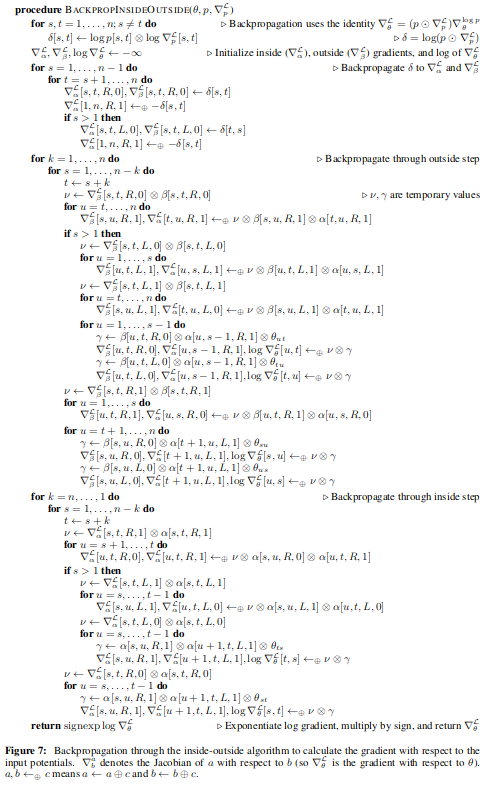
\includegraphics[height=.7\textheight]{img/backprop-inside-outside.png}}}
\end{frame}
\againframe<8-9>{mainidea}
\begin{frame}<1>[label=smapsolution]
\cornercite{sparsemap}%
\frametitle{SparseMAP solution}
\makebox[\textwidth][c] {
\renewcommand{\arraystretch}{3}
\begin{tabular}{r@{~=~}l}
    $\mg^\star$ & $\displaystyle \argmax_{\mg \in \Mp} \mg ^\top \pr - \nicefrac{1}{2} \|\mg\|^2$ \\
    &\cartoonSparse[.7] $=~.6$ \cartoon[.7]{1/4,2/5} $+~.4$
    \cartoon[.7]{1/4,1/5} %\\
%    &$\bs{A}\p^\star$ with very sparse $\p^\star \in \triangle^N$
\end{tabular}
}
\centering
{\small ($\mg^\star$ is unique, but may have multiple decompositions $\p$. Active Set
recovers a sparse one.)}
\end{frame}
%
%
\begin{frame}
%
\frametitle{Algorithms for SparseMAP}
%
\vspace{-1.5\baselineskip}
\uncover<1->{
\[\mg^\star = \argmax_{\tikzmark{constr}\mg \in \Mp} \mg ^\top \pr
 -\nicefrac{1}{2} \|\mg\|^2\tikzmark{quadr}\]}
\\[\baselineskip]
\begin{columns}%
\fontsize{12pt}{14}\selectfont%
\uncover<3->{
\begin{column}{.5\textwidth}%
\vbox to .5\textheight{%
\centering
\textbf{Conditional Gradient} \\
\citep{fw,cg}
\begin{itemize}
    \item<4-> select a new corner of $\Mp$
    \item<6-> update the (sparse) coefficients of $\p$
        \begin{itemize}
            \item<6-> Update rules: vanilla, away-step, pairwise
            \item<7-> Quadratic objective: \textbf{Active Set}\\
a.k.a.\ Min-Norm Point, \citep{mnp}\\
\citep{ad3,nocedalwright,vinyes}
%\color{mygr}{\scriptsize\parencite[][Ch.~16.4 \& 16.5]{nocedalwright}}\\
%\color{mygr}\citep[][Ch.~16.4 \& 16.5]{nocedalwright}}\\

\end{itemize}
\end{itemize}
}\end{column}}
\uncover<9->{%
\begin{column}{.5\textwidth}%
\vbox to .5\textheight{%
\centering
\textbf{Backward pass}\\[2\baselineskip]
$\frac{\partial \mg}{\partial \pr}$ is sparse\\
\uncover<10->{%
computing $\left(\frac{\partial \mg}{\partial \pr}\right)^\top \bs{d}y$ \\
takes $\mathcal{O}(\operatorname{dim}(\mg)\operatorname{nnz}(\p^\star))$}
}\end{column}}
\end{columns}
\begin{tikzpicture}[%
    remember picture,
    overlay,
    expl/.style={font=\small}]
\uncover<2->{
    \node[expl,anchor=north east] (explquadr)
        at ($(current page.north east) - (.5, 2)$)
        {quadratic objective};
    \path (explquadr.west) edge[->,very thick,bend left] ([yshift=-0.5ex]{pic cs:quadr});
}
\uncover<2->{
    \node[expl,anchor=north west,align=left] (explconstr)
        at ($(current page.north west) + (.5, -2)$)
        {linear constraints\\%
         \textcolor{mygr}{\emph{(alas, exponentially many!)}}};
    \path (explconstr.south east) edge[->,very thick,bend right] ([yshift=-1ex]{pic cs:constr});
}
\end{tikzpicture}
\uncover<5>{\overlaybox[.8]{
        $\displaystyle \argmax_{\mg \in \Mp} \mg^\top~
\underbrace{(\pr - \mg^{(t-1)})}_{\widetilde\pr}$
}}
\uncover<8>{\overlaybox{Active Set achieves \\ \textbf{finite} \&
    \textbf{linear} convergence!}}
\uncover<11>{\overlaybox[.5]{Completely modular: just add MAP}}
\end{frame}

{
\setbeamercolor{background canvas}{bg=myfg}
\setbeamercolor{normal text}{fg=mybg}
\setbeamercolor{frametitle}{fg=mybg}
\usebeamercolor[fg]{frametitle}
\usebeamercolor[fg]{normal text}
\begin{frame}[plain]%
\cornercite{esim}%
\hspace{1ex}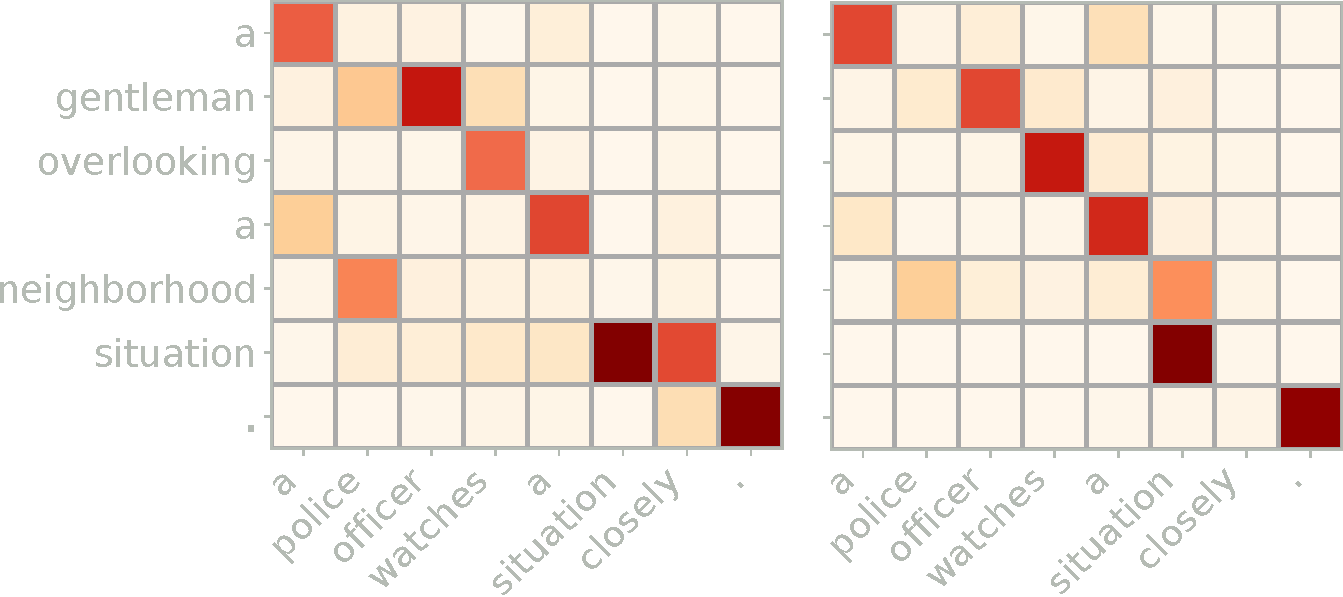
\includegraphics[height=.7\textheight]{img/snli_softmax.pdf}
\end{frame}

\newcommand*\transpmatch[3]{
\foreach[count=\i] \j in {#3}%
\draw[tPeony,thick, opacity=#1,
      {Circle[length=.6mm,width=.6mm]}-{Circle[length=.6mm, width=.6mm]}]
      ($(s\i.east) + (0, #2)$) -- ($(t\j.west) + (0, #2)$);
}
\begin{frame}[plain]%
\cornercite{sparsemap}%
\hspace{1ex}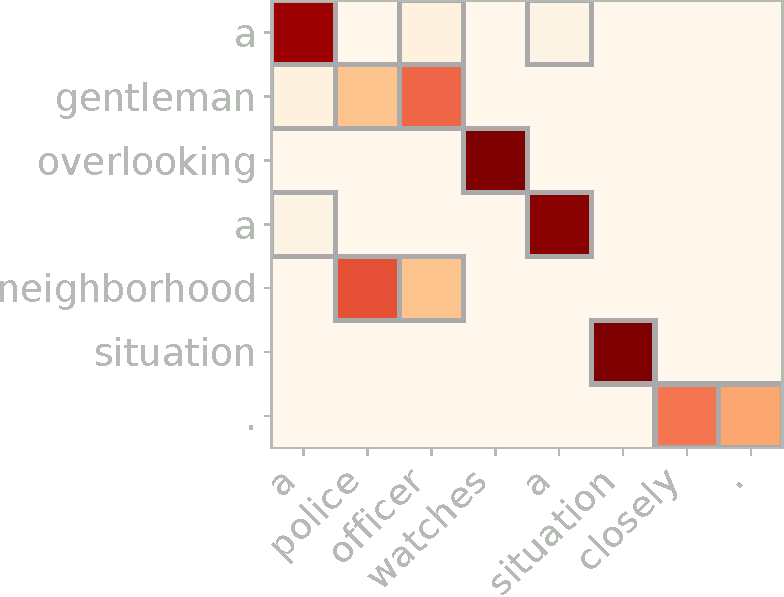
\includegraphics[height=.7\textheight]{img/snli_matching.pdf}%
%
%
\raisebox{3ex}{%
\def\xp{0}%
\def\xh{2}%
\def\baseh{0}%
\def\basep{0.3}%
\def\H{0.7}%
\footnotesize%
%
\begin{tikzpicture}%
\node[anchor=east] at (\xp, \basep+6*\H) (s1) {A};
\node[anchor=east] at (\xp, \basep+5*\H) (s2) {gentleman};
\node[anchor=east] at (\xp, \basep+4*\H) (s3) {overlooking};
\node[anchor=east] at (\xp, \basep+3*\H) (s4) {a};
\node[anchor=east] at (\xp, \basep+2*\H) (s5) {neighborhood};
\node[anchor=east] at (\xp, \basep+1*\H) (s6) {situation};
\node[anchor=east] at (\xp, \basep+0*\H) (s7) {.};
%
\node[anchor=west] at (\xh, \baseh+7*\H) (t1) {A};
\node[anchor=west] at (\xh, \baseh+6*\H) (t2) {police};
\node[anchor=west] at (\xh, \baseh+5*\H) (t3) {officer};
\node[anchor=west] at (\xh, \baseh+4*\H) (t4) {watches};
\node[anchor=west] at (\xh, \baseh+3*\H) (t5) {a};
\node[anchor=west] at (\xh, \baseh+2*\H) (t6) {situation};
\node[anchor=west] at (\xh, \baseh+1*\H) (t7) {closely};
\node[anchor=west] at (\xh, \baseh+0*\H) (t8) {.};


\transpmatch{.1}{-4pt}{5,2,4,1,3,6,8}%
\transpmatch{.2}{-2pt}{3,1,4,5,2,6,8}%
\transpmatch{.2}{-0pt}{1,3,4,5,2,6,8}%
\transpmatch{.8}{+2pt}{1,2,4,5,3,6,8}%
\transpmatch{1}{+4pt}{1,3,4,5,2,6,7}%

\end{tikzpicture}}
\end{frame}}


\againframe<4>{overview}

\begin{frame}%
\newcommand*\parcolor{myfg}
\newcommand*\clfcolor{myfg}
\newcommand*\colParseZero{mybg}
\newcommand*\colParseNonz{mybg}
\only<2->{
\renewcommand*\parcolor{tPink}
\renewcommand*\clfcolor{tDY}
}
\only<14->{
\renewcommand*\colParseZero{mybg!25!box}
\renewcommand*\colParseNonz{mybg}
}
\frametitle{Structured latent variables without sampling}
\begin{align*}
    \EE_{\z}\big[L(\z)\big] &= \tikzmark{sum}\sum_{\z \in \ZZ}
    \textcolor{\clfcolor}{L\big(\hat{y}\tikzmark{clfp}_{\uncover<2->{\clfp}}(\z)\big)}~%
    \textcolor{\parcolor}{\pi\tikzmark{parp}_{\uncover<2->{\parp}}(\z \mid x)}%
% \\
%    \uncover<3->{
%        &= \EE_{h \sim \textcolor{\parcolor}{p_{\parp}(h \mid x)}}~%
%        \textcolor{\clfcolor}{p_{\clfp}(y\mid h, x)}
%    }
\end{align*}
%\vspace{.2\baselineskip}
\vfill
\makebox[\textwidth][c]{%
\begin{minipage}{\textwidth}\centering
\par
\fontsize{12pt}{14}\selectfont%
{%
\uncover<6->{%
\textbf{How to define {\boldmath $\textcolor{\parcolor}{\pi_{\parp}}$}?}%
}
\par
\renewcommand{\arraystretch}{1.25}
\begin{tabular}{r l c c c c}
& & &
\uncover<7->{$\displaystyle \sum_{h \in \mathcal{H}}$} &
\uncover<8->{$\displaystyle \pfrac{\EE\big[L(\z)\big]}{\textcolor{\parcolor}{\parp}}$}
\\
\uncover<6->{\textcolor{mygr}{idea 1}} &
\uncover<9->{$\textcolor{\parcolor}{\pi_{\parp}(\z)}
\propto \exp \big( f_{\parp}(\z) \big) $}
& \uncover<9->{softmax}
& \uncover<11->{\emoji{oface}}
& \uncover<10->{\emoji{happ}} \\
\uncover<6->{\textcolor{mygr}{idea 2}} &
\uncover<13->{$\textcolor{\parcolor}{\pi_{\parp}(\z)} = 1$ if $\z =
\operatorname{MAP}(f_{\parp}(\cdot))$ else $0$}
& \uncover<13->{argmax}
& \uncover<14->{\emoji{happ}}
& \uncover<15->{\emoji{frown}} \\
%
\uncover<6->{\textcolor{mygr}{idea 3}} &
& \uncover<17->{SparseMAP} & \uncover<17->{\emoji{happ}} & \uncover<17->{\emoji{happ}}
\end{tabular}%
}%
\end{minipage}}

\begin{tikzpicture}[%
    remember picture,
    overlay,
    expl/.style={font=\small}]
\uncover<3->{
    \node[expl,anchor=north east] (explpar)
        at ($(current page.north east) - (.5, 1.5)$)
        {\emph{e.g.},\ a TreeLSTM defined by $\z$};
    \path (explpar.west) edge[->,very thick,bend right] ([yshift=1.5ex]{pic cs:clfp});
}
%
\uncover<5->{
    \node[expl,anchor=north west,align=left] (explsum)
        at ($(current page.north west) + (.5, -1.5)$)
        {sum over \\ all possible trees};
    \path (explsum.east) edge[->,very thick,bend left] ([yshift=2.5ex]{pic cs:sum});
}
\uncover<4->{
    \node[expl,anchor=north east,align=right] (explscore)
        at ($(current page.north east) - (.5, 4)$)
        {parsing model,\\using some scorer $f_{\parp}(\z;x)$};
    \path (explscore.west) edge[->,very thick,bend left] ([yshift=-.5ex]{pic cs:parp});
}

% HERE highlight
% \uncover<10>{%
%     \draw[
%         tBlue,
%         opacity=.5,
%         ultra thick]
%         ($(pic cs:argmax1)!.5!(pic cs:argmax2)$) ellipse (1cm and .5cm);
% }
\end{tikzpicture}%
\uncover<5>{\overlaybox[.8]{Exponentially large sum!}}
\uncover<12>{\overlaybox{All methods we've seen require sampling; hard in
general.}}
\uncover<16>{\overlaybox{STE / SPIGOT relax $\hat{y}$ in backward.}}
\end{frame}


\begin{frame}
\newcommand*\clfColor{tDY}
\frametitle{Structured latent variables without sampling}
\centering
\begin{tabular}{r@{~~}l@{\,}l@{}l@{\,}l@{\,}l@{\,}l@{\,}l}
    \miniparse{a/b/l/.7,a/c/l/1,c/b/r/.4}$ =$
    & $.7\times$ & \miniparse{a/b/l/1,a/c/l/1} & &+  $.3\times$&  \miniparse{c/b/r/1,a/c/l/1}
    & \uncover<2->{ $+ 0\times$} &
    \uncover<2->{\miniparse{a/b/l/1,b/c/l/1} + ...}
    \\
\uncover<3->{
     $\EE[L(\z)] =$ &
     $.7\times$ \textcolor{\clfColor}{$L($} &
     \miniparse{a/b/l/1,a/c/l/1} &
     \textcolor{\clfColor}{$)$}&+ $.3\times$ \textcolor{\clfColor}{$L($} &
     \miniparse{c/b/r/1,a/c/l/1} &
     \textcolor{\clfColor}{$)$}&
}
\end{tabular}
\\[2\baselineskip]
{
\small
\textcolor{mygr}{recall our shorthand}
$L(\z) = L(\hat{y}_{\clfp}(\z), y)$
}
\end{frame}
%
\begin{frame}
\cornercite{corro2019acl}
\small
\begin{columns}
\begin{column}{.4\textwidth}
\centering {Stanford Sentiment (Accuracy)} \\[1ex]
\begin{tabular}{l r}
\multicolumn{2}{l}{Socher et al} \\
Bigram Naive Bayes     & 83.1 \\[.3ex]
\multicolumn{2}{l}{\citep{sparsemapcg}} \\
TreeLSTM w/ CoreNLP    & 83.2 \\
TreeLSTM w/ SparseMAP  & 84.7 \\[.3ex]
\multicolumn{2}{l}{\citep{corro2019acl}} \\
GCN w/ CoreNLP         & 83.8 \\
GCN w/ Perturb-and-MAP & 84.6
\end{tabular}
\end{column}
\begin{column}{.6\textwidth}
\centering {Stanford Natural Language Inference (Accuracy)} \\[1ex]
\begin{tabular}{l r}
\multicolumn{2}{l}{\citep{structured_attn}} \\
Simple Attention & 86.2 \\
Structured Attention & 86.8 \\[.3ex]
\multicolumn{2}{l}{\citep{lapata}} \\
100D SAN - & 86.8 \\[.3ex]
\multicolumn{2}{l}{Yogatama et al} \\
100D RL-SPINN     & 80.5 \\[.3ex]
\multicolumn{2}{l}{\citep{choi2017learning}} \\
100D ST Gumbel-Tree & 82.6 \\
300D - & 85.6 \\
600D - & 86.0 \\[.3ex]
\multicolumn{2}{l}{\citep{corro2019acl}} \\
Latent Tree + 1 GCN - & 85.2 \\
Latent Tree + 2 GCN - & 86.2 \\[.3ex]
\end{tabular}
\end{column}
\end{columns}
\end{frame}
%

\section{Conclusions}
\sepframe{V. Conclusions}
\begin{frame}
\frametitle{Is it syntax?!}
\begin{itemize}
\item Unlike e.g.\ unsupervised parsing, the structures we learn are guided by
\textbf{a downstream objective} (typically discriminative).
\item<+-> They don't typically resemble grammatical structure (yet)
\citep{isitsyntax}\\
\quad(future work: more inductive biases and constraints?)
\item<+-> Common to compare latent structures with parser outputs. \\\quad But is
this always a meaningful comparison?
\end{itemize}
\end{frame}

\depstyle{mydep}{edge style={tPeony,thick},arc edge,hide label}
\begin{frame}
\frametitle{Syntax vs.\ Composition Order}
\cornercite{sparsemapcg}
\centering
\uncover<2->{
{\small $p=22.6\%$}\\
\begin{dependency}[mydep]
\begin{deptext}[column sep=0.3cm]
$\star$ \& lovely \& and \& poignant \& . \\ \end{deptext}
\depedge{3}{2}{}
\depedge{1}{3}{}
\depedge{3}{4}{}
\depedge{3}{5}{}
\end{dependency}}
\\
\uncover<1->{
{\small CoreNLP parse,\quad$p=21.4\%$}\\
\begin{dependency}[mydep]
\begin{deptext}[column sep=0.3cm]
$\star$ \& lovely \& and \& poignant \& . \\ \end{deptext}
\depedge{1}{2}{}
\depedge{2}{3}{}
\depedge{2}{4}{}
\depedge{2}{5}{}
\end{dependency}}\\
\uncover<2->{$\cdots$}
\end{frame}
\begin{frame}
\frametitle{Syntax vs.\ Composition Order}
\cornercite{sparsemapcg}
\fontsize{9pt}{10}\selectfont%
\centering
\begin{columns}
\begin{column}{.5\textwidth}
\centering
{$p=22.6\%$}\\
\begin{dependency}[mydep]
\begin{deptext}[column sep=0.3cm]
$\star$ \& lovely \& and \& poignant \& . \\ \end{deptext}
\depedge{3}{2}{}
\depedge{1}{3}{}
\depedge{3}{4}{}
\depedge{3}{5}{}
\end{dependency}
\\[\baselineskip]
{CoreNLP parse,\quad$p=21.4\%$}\\
\begin{dependency}[mydep]
\begin{deptext}[column sep=0.3cm]
$\star$ \& lovely \& and \& poignant \& . \\ \end{deptext}
\depedge{1}{2}{}
\depedge{2}{3}{}
\depedge{2}{4}{}
\depedge{2}{5}{}
\end{dependency}\\
$\cdots$
\end{column}
\begin{column}{.5\textwidth}
\centering
{$p=15.33\%$}\\
\begin{dependency}[mydep,arc angle=35]
\begin{deptext}[column sep=0.3cm]
$\star$ \& a \& deep \& and \& meaningful \& film \& . \\ \end{deptext}
\depedge{1}{2}{1.0}
\depedge{1}{3}{1.0}
\depedge{1}{4}{1.0}
\depedge{1}{5}{1.0}
\depedge{1}{6}{1.0}
\depedge{1}{7}{1.0}
\end{dependency}\\[\baselineskip]
{$p=15.27\%$}\\
\begin{dependency}[mydep,arc angle=50]
\begin{deptext}[column sep=0.3cm]
$\star$ \& a \& deep \& and \& meaningful \& film \& . \\ \end{deptext}
\depedge{4}{2}{1.0}
\depedge{4}{3}{1.0}
\depedge{1}{4}{1.0}
\depedge{4}{5}{1.0}
\depedge{4}{6}{1.0}
\depedge{4}{7}{1.0}
\end{dependency}\\
{$\cdots$\\ CoreNLP parse,\quad$p=0\%$}\\
\begin{dependency}[mydep,arc angle=35]
\begin{deptext}[column sep=0.3cm]
$\star$ \& a \& deep \& and \& meaningful \& film \& . \\ \end{deptext}
\depedge{6}{2}{1.0}
\depedge{6}{3}{1.0}
\depedge{3}{4}{1.0}
\depedge{3}{5}{1.0}
\depedge{1}{6}{1.0}
\depedge{6}{7}{1.0}
\end{dependency}
\end{column}
\end{columns}
\end{frame}

\againframe<5->{overview}

\begin{frame}
\frametitle{Conclusions}
\begin{itemize}
\item Latent structure models are desirable for interpretability, structural bias, and higher predictive power with fewer parameters.
\item Stochastic latent variables can be dealt with RL or straight-through gradients.
\item Deterministic argmax requires surrogate gradients (e.g. SPIGOT).
\item Continuous relaxations of argmax include SANs and SparseMAP.
\item Intuitively, some of these different methods are trying to do similar
things or require the same building blocks (e.g. SPIGOT and
SparseMAP).\\[.5\baselineskip]
\item ... we didn't even get into deep \emph{generative} models! These tools
apply,\\but there are new challenges.
\citep{corro2018differentiable,rnng2,rnng1,segm}
\end{itemize}
\end{frame}



\begin{frame}[t,allowframebreaks]
\frametitle{References}
\scriptsize
\bibliographystyle{plainnat}
\bibliography{refs}
\end{frame}

\end{document}
